\section{CHƯƠNG 1: GIỚI THIỆU ĐỀ TÀI}

\subsection{Giới thiệu đề tài}
Trong quá trình quản lý dự án, việc tổ chức và theo dõi công việc luôn là một bài toán phức tạp đối với các cá nhân hay tổ chức. Khi số lượng công việc gia tăng, các phương pháp quản lý truyền thống hoặc rời rạc thường bộc lộ nhiều hạn chế, dẫn đến những khó khăn trực tiếp trong việc kiểm soát tiến độ, phân chia nguồn lực và duy trì sự phối hợp giữa các thành viên. Tình trạng thất lạc thông tin, thiếu minh bạch về trạng thái thực hiện các hạng mục công việc làm suy giảm đáng kể hiệu suất chung. Xuất phát từ thực trạng này, bài toán đặt ra là cần xây dựng một giải pháp phần mềm hỗ trợ quản lý dự án tập trung, trực quan, giúp người dùng dễ dàng tổ chức các đầu việc, theo dõi tiến độ và nâng cao hiệu quả cộng tác.

\subsection{Tính cấp thiết của đề tài}
Hiện nay, mặc dù đã có nhiều giải pháp phần mềm hỗ trợ quản lý, nhiều cá nhân và tổ chức tại Việt Nam vẫn sử dụng các phương pháp thủ công như ghi chép sổ tay, bảng trắng, hoặc các công cụ kỹ thuật số rời rạc và thiếu tính trực quan như email, bảng tính Excel, hay các ứng dụng nhắn tin nhanh. Các phương thức tiếp cận truyền thống này bộc lộ nhiều hạn chế nghiêm trọng trong môi trường làm việc hiện đại:
\begin{itemize}
    \item \textbf{Thất lạc và phân mảnh thông tin:} Các yêu cầu công việc, phản hồi và tài liệu đính kèm bị phân tán trên nhiều kênh giao tiếp khác nhau, dẫn đến khó khăn trong việc tìm kiếm và dễ bỏ sót nhiệm vụ.
    \item \textbf{Khó theo dõi tiến độ tổng thể:} Người quản lý và các thành viên gặp nhiều khó khăn để có được cái nhìn tổng quan về trạng thái hiện tại của dự án, dẫn đến chậm trễ tiến độ mà không có biện pháp cảnh báo hoặc xử lý kịp thời.
    \item \textbf{Thiếu tính tương tác trực quan:} Các công cụ truyền thống không hỗ trợ cập nhật động trạng thái công việc và luồng di chuyển của các nhiệm vụ theo thời gian thực.
    \item \textbf{Giảm hiệu suất cộng tác nhóm:} Việc phân chia trách nhiệm và giao việc không được định nghĩa rõ ràng, gây chồng chéo công việc và suy giảm hiệu quả làm việc chung.
\end{itemize}
Từ những hạn chế trên, việc nghiên cứu và xây dựng ``Hệ thống quản lý công việc'' là vô cùng cấp thiết. Hệ thống được phát triển nhằm khắc phục các nhược điểm của phương pháp truyền thống bằng việc cung cấp một giao diện quản lý trực quan theo mô hình Kanban. Giải pháp này giúp chuẩn hóa quy trình giao việc, nâng cao tính minh bạch trong tập thể, tối ưu hóa quy trình làm việc và giảm thiểu tối đa các sai sót thông tin trong suốt quá trình vận hành dự án.

\subsection{Mục tiêu đề tài}
Mục tiêu chính của đề tài là nghiên cứu, thiết kế và phát triển một nền tảng quản lý công việc và thẻ công việc (task/card) hiệu quả, trực quan, dễ tiếp cận và có khả năng tương tác cao. Các mục tiêu chi tiết bao gồm:
\begin{itemize}
    \item \textbf{Xây dựng nền tảng quản lý khoa học:} Cho phép người dùng dễ dàng tổ chức công việc theo các không gian làm việc (workspace) riêng biệt và các bảng công việc (board) theo từng dự án cụ thể.
    \item \textbf{Quản lý thẻ công việc chi tiết:} Cung cấp đầy đủ các thuộc tính quản lý cho một nhiệm vụ như tiêu đề, mô tả chi tiết, gán thành viên thực hiện, thiết lập thời hạn hoàn thành (due date) và xây dựng các danh sách kiểm tra công việc con (checklist) để theo dõi chi tiết.
    \item \textbf{Tích hợp cơ chế tương tác trực quan:} Triển khai thành công tính năng kéo thả (drag and drop) các thẻ công việc giữa các danh sách trạng thái khác nhau, mang lại trải nghiệm mượt mà và trực quan cho người dùng.
    \item \textbf{Đồng bộ dữ liệu và cộng tác hiệu quả:} Đảm bảo các cập nhật về trạng thái công việc, phân công nhân sự và thời hạn được đồng bộ hóa nhanh chóng đến toàn bộ thành viên trong bảng công việc.
\end{itemize}

\subsection{Phạm vi đề tài}
Đề tài tập trung nghiên cứu và triển khai các chức năng cốt lõi phục vụ nhu cầu quản lý công việc hàng ngày của cá nhân và đội ngũ, cụ thể bao gồm:
\begin{itemize}
    \item \textbf{Hệ thống xác thực và quản lý tài khoản:} Triển khai các tính năng đăng ký, đăng nhập, đăng xuất và cập nhật thông tin cá nhân của người dùng, tích hợp giải pháp xác thực bảo mật thông qua dịch vụ điện toán đám mây Amazon Cognito.
    \item \textbf{Quản lý Workspace:} Tạo lập, cập nhật thông tin, xóa và tổ chức các không gian làm việc để quản lý tập trung nhiều dự án liên quan.
    \item \textbf{Quản lý Board:} Tạo mới, cập nhật thông tin, xóa các bảng công việc theo dự án; triển khai tính năng tìm kiếm và thêm thành viên vào bảng công việc.
    \item \textbf{Quản lý danh sách công việc (List):} Tạo mới, đổi tên, thay đổi thứ tự sắp xếp và xóa các danh sách trong mỗi bảng nhằm phân loại trạng thái công việc (ví dụ: Cần làm, Đang làm, Đã hoàn thành).
    \item \textbf{Quản lý thẻ công việc (Card):} Thực hiện các thao tác CRUD (Tạo, Đọc, Cập nhật, Xóa) đối với thẻ công việc; hỗ trợ thêm mô tả chi tiết, gán thành viên chịu trách nhiệm, thiết lập thời hạn hoàn thành và hiển thị trạng thái cảnh báo trực quan khi công việc sắp đến hạn hoặc quá hạn.
    \item \textbf{Quản lý danh sách kiểm tra (Checklist):} Cho phép tạo các checklist trong mỗi card, thêm các hạng mục công việc con (checklist item), đánh dấu hoàn thành/chưa hoàn thành và hiển thị thanh tiến độ (progress bar) trực quan theo tỷ lệ phần trăm hoàn thành.
    \item \textbf{Tương tác kéo thả (Drag and Drop):} Phát triển thuật toán và giao diện hỗ trợ kéo thả thẻ công việc giữa các danh sách hoặc thay đổi vị trí của các thẻ trong cùng một danh sách, đảm bảo tính nhất quán về vị trí hiển thị giữa Frontend và Backend.
\end{itemize}
Các nội dung và tính năng nằm ngoài phạm vi nghiên cứu thực hiện của học phần bao gồm:
\begin{itemize}
    \item Các chức năng phân tích số liệu nâng cao, dự báo tiến độ và tự động xuất các báo cáo thống kê định kỳ dưới dạng biểu đồ phức tạp.
    \item Việc tích hợp sâu hệ thống quản lý công việc với các nền tảng và dịch vụ của bên thứ ba như Slack, Google Calendar, hay các công cụ lưu trữ đám mây bên ngoài.
    \item Tối ưu hóa hạ tầng và cơ chế cân bằng tải để phục vụ cho hệ thống quy mô lớn có hàng triệu người dùng hoạt động đồng thời.
\end{itemize}

\subsection{Đối tượng sử dụng}
Hệ thống quản lý công việc hướng đến việc giải quyết nhu cầu của các nhóm đối tượng người dùng chính sau:
\begin{itemize}
    \item \textbf{Cá nhân:} Người dùng có nhu cầu sắp xếp, lên kế hoạch và quản lý các công việc học tập, nghiên cứu hoặc làm việc cá nhân hàng ngày một cách khoa học, giúp tăng tính kỷ luật và hiệu suất cá nhân.
    \item \textbf{Nhóm làm việc và phòng ban:} Các đội ngũ phát triển dự án, nhóm nghiên cứu hoặc các phòng ban chức năng trong tổ chức cần một không gian cộng tác số thống nhất để phân công công việc, phối hợp thực hiện và cùng theo dõi tiến độ công việc một cách minh bạch, rõ ràng.
    \item \textbf{Quản lý dự án:} Những người chịu trách nhiệm điều phối và giám sát toàn bộ hoạt động của dự án, cần theo dõi tổng quan tiến độ của từng hạng mục công việc, kiểm soát thời hạn hoàn thành (deadlines) và tối ưu hóa việc phân bổ nguồn lực nhân sự.
\end{itemize}
\clearpage

\setcounter{secnumdepth}{4}
\setcounter{tocdepth}{4}
\section{CHƯƠNG 2: CƠ SỞ LÝ THUYẾT}

\subsection{Cách tiếp cận và hướng giải quyết}

\subsubsection{Phương pháp phân tích bài toán}
Bài toán được tiếp cận theo hướng phân tích từ trên xuống (top-down), bắt đầu từ việc nghiên cứu các hệ thống quản lý công việc phổ biến hiện có trên thị trường như Trello và Jira, từ đó xác định mô hình nghiệp vụ, các thực thể dữ liệu cốt lõi và luồng hoạt động của hệ thống. Qua nghiên cứu, mô hình Kanban được lựa chọn làm nền tảng tổ chức công việc do tính trực quan và khả năng phản ánh trạng thái công việc một cách rõ ràng theo các cột trạng thái (To Do, In Progress, Done).

Mô hình dữ liệu nghiệp vụ được xác định xoay quanh sáu thực thể chính theo cấu trúc phân cấp:
\begin{itemize}
    \item \textbf{Workspace}: không gian làm việc tổng thể của người dùng, quản lý tập trung nhiều dự án liên quan.
    \item \textbf{Board}: đại diện cho một dự án hoặc bảng công việc cụ thể bên trong Workspace.
    \item \textbf{List}: các cột trạng thái bên trong Board, thể hiện giai đoạn thực hiện của công việc.
    \item \textbf{Card}: nhiệm vụ cụ thể cần thực hiện, được đặt trong các List tương ứng.
    \item \textbf{Checklist}: danh sách các công việc con nằm bên trong thẻ công việc (Card), hỗ trợ theo dõi chi tiết tiến trình thực hiện.
    \item \textbf{ChecklistItem}: các hạng mục cụ thể bên trong Checklist, có thể được đánh dấu trạng thái hoàn thành.
\end{itemize}

\subsubsection{Hướng thiết kế giải pháp}
Giải pháp được thiết kế theo kiến trúc client-server với sự tách biệt rõ ràng giữa Frontend và Backend thông qua giao tiếp RESTful API. Hướng tiếp cận này giúp hai thành phần có thể phát triển song song, dễ dàng bảo trì và mở rộng độc lập. Toàn bộ logic nghiệp vụ được tập trung xử lý tại Backend, trong khi Frontend chịu trách nhiệm trình bày giao diện và tương tác với người dùng.

\subsubsection{Các quyết định kỹ thuật chính}
Các quyết định kỹ thuật quan trọng được đưa ra trong quá trình thiết kế hệ thống bao gồm:
\begin{itemize}
    \item \textbf{Phân tách Frontend và Backend}: Frontend xây dựng bằng ReactJS, Backend xây dựng bằng Java Spring Boot, giao tiếp qua REST API, tạo ra sự linh hoạt cao trong phát triển và triển khai.
    \item \textbf{Ủy quyền xác thực cho dịch vụ bên thứ ba}: Sử dụng Amazon Cognito để quản lý toàn bộ vòng đời người dùng (đăng ký, xác thực email, đăng nhập), giúp Backend tập trung vào logic nghiệp vụ thay vì tự xử lý xác thực.
    \item \textbf{Lưu trữ token bằng HttpOnly Cookie}: Access token và refresh token được lưu trong HttpOnly cookie thay vì localStorage, ngăn chặn các cuộc tấn công XSS (Cross-Site Scripting).
    \item \textbf{Cơ sở dữ liệu quan hệ PostgreSQL}: Phù hợp với mô hình dữ liệu có cấu trúc quan hệ rõ ràng và hỗ trợ tốt cho JPA/Hibernate trong Spring Boot.
    \item \textbf{Triển khai trên nền tảng Cloud}: Ứng dụng được triển khai hoàn toàn lên môi trường điện toán đám mây thông qua hệ sinh thái các dịch vụ của AWS (bao gồm EC2, RDS, S3, CloudFront và ALB), giúp hệ thống tận dụng tối đa khả năng mở rộng linh hoạt, tối ưu chi phí hạ tầng và đảm bảo tính sẵn sàng cao.
\end{itemize}

\subsection{Các nền tảng và công nghệ sử dụng}

\subsubsection{Các nền tảng liên quan đến ứng dụng}

\paragraph{ReactJS}

\begin{itemize}
    \item \textbf{Giới thiệu:} ReactJS là thư viện JavaScript mã nguồn mở được phát triển bởi Meta (Facebook), chuyên dùng để xây dựng giao diện người dùng (UI) tương tác và có hiệu suất cao.
\begin{figure}[H]
    \centering
    
\includegraphics[width=0.5\textwidth]{./images/chap2/React.jpg}
    \caption{Logo ReactJS}
    \label{fig:reactjs_logo}
\end{figure}
    \item \textbf{Chức năng:} ReactJS hoạt động theo cơ chế component-based, cho phép chia nhỏ giao diện thành các thành phần độc lập, có thể tái sử dụng. Virtual DOM giúp cập nhật giao diện một cách hiệu quả bằng cách chỉ render lại những phần thực sự thay đổi, thay vì cập nhật toàn bộ cây DOM.
    \item \textbf{Vai trò trong hệ thống:} ReactJS được sử dụng để xây dựng toàn bộ tầng giao diện (View layer) của hệ thống quản lý công việc, bao gồm các màn hình xác thực (đăng ký, đăng nhập), màn hình Dashboard hiển thị danh sách Workspace và Board, cũng như màn hình Board chi tiết với các chức năng quản lý List, Card và Drag and Drop.
    \item \textbf{Lý do lựa chọn:} Đối với các dạng ứng dụng web trang đơn (Single Page Application - SPA), ReactJS là một thư viện phổ biến, được sử dụng rất nhiều bởi các lập trình viên nhờ tính linh hoạt và khả năng triển khai dễ dàng, nhanh chóng.
\end{itemize}

\paragraph{Java Spring Boot}

\begin{itemize}
    \item \textbf{Giới thiệu:} Spring Boot là framework phát triển ứng dụng Java được xây dựng trên nền tảng Spring Framework, cung cấp cơ chế tự động cấu hình (auto-configuration) giúp giảm thiểu thời gian thiết lập dự án và tập trung vào triển khai logic nghiệp vụ.
\begin{figure}[H]
    \centering
    
\includegraphics[width=0.5\textwidth]{./images/chap2/SpringBoot.jpg}
    \caption{Logo Java Spring Boot}
    \label{fig:springboot_logo}
\end{figure}
    \item \textbf{Chức năng:} Spring Boot hỗ trợ xây dựng các ứng dụng RESTful API thông qua module Spring Web, quản lý kết nối cơ sở dữ liệu thông qua Spring Data JPA và Hibernate, đồng thời cung cấp cơ chế dependency injection giúp tổ chức code theo hướng lập trình hướng đối tượng rõ ràng.
    \item \textbf{Vai trò trong hệ thống:} Spring Boot đóng vai trò là tầng Backend của hệ thống, xử lý toàn bộ logic nghiệp vụ, xây dựng và cung cấp các RESTful API cho Frontend tiêu thụ. Cấu trúc project được tổ chức theo mô hình phân lớp bao gồm: \texttt{controller}, \texttt{service}, \texttt{repository} và \texttt{config}.
    \item \textbf{Lý do lựa chọn:} Spring Boot là một framework hỗ trợ công việc viết code cho các lập trình viên một cách mạnh mẽ và tối ưu. Kết hợp cùng với Java - một ngôn ngữ lập trình chặt chẽ, có tính ổn định cao, việc sử dụng Spring Boot giúp giảm thiểu tối đa các lỗi hệ thống có thể xảy ra trong quá trình vận hành.
\end{itemize}

\paragraph{PostgreSQL}

\begin{itemize}
    \item \textbf{Giới thiệu:} PostgreSQL là hệ quản trị cơ sở dữ liệu quan hệ mã nguồn mở mạnh mẽ, hỗ trợ đầy đủ các tính năng của SQL chuẩn cùng nhiều tính năng nâng cao như kiểu dữ liệu JSON, UUID, các ràng buộc phức tạp.
\begin{figure}[H]
    \centering
    
\includegraphics[width=0.5\textwidth]{./images/chap2/PostgreSQL.png}
    \caption{Logo PostgreSQL}
    \label{fig:postgresql_logo}
\end{figure}
    \item \textbf{Chức năng:} PostgreSQL đảm bảo tính toàn vẹn dữ liệu thông qua các ràng buộc FK (foreign key), hỗ trợ các truy vấn phức tạp với nhiều bảng quan hệ, đồng thời cung cấp hiệu suất đọc/ghi ổn định phù hợp với các ứng dụng web thông thường.
    \item \textbf{Vai trò trong hệ thống:} PostgreSQL được sử dụng làm hệ quản trị cơ sở dữ liệu chính của hệ thống, lưu trữ toàn bộ dữ liệu nghiệp vụ bao gồm thông tin người dùng, Workspace, Board, List, Card, Checklist và các bảng quan hệ trung gian. Kết nối với Backend thông qua Spring Data JPA và trình điều khiển PostgreSQL JDBC.
\end{itemize}

\paragraph{Mô hình MVC (Model -- View -- Controller)} \mbox{}\\

MVC là mẫu kiến trúc phần mềm (architectural pattern) phân tách ứng dụng thành ba thành phần độc lập: \textbf{Model} chịu trách nhiệm quản lý dữ liệu và logic nghiệp vụ; \textbf{View} đảm nhận việc trình bày dữ liệu ra giao diện người dùng; \textbf{Controller} đóng vai trò trung gian, tiếp nhận yêu cầu từ người dùng, điều phối Model xử lý và trả kết quả về View.


\subsubsection{Các nền tảng liên quan đến dịch vụ đám mây}

\paragraph{Amazon Cognito}
\begin{itemize}
    \item \textbf{Giới thiệu:} Amazon Cognito là dịch vụ quản lý danh tính và xác thực người dùng do Amazon Web Services (AWS) cung cấp, hỗ trợ các luồng xác thực theo chuẩn OAuth 2.0 và OpenID Connect.
    \item \textbf{Chức năng:} Amazon Cognito cung cấp hai thành phần chính: User Pool để quản lý người dùng và xác thực danh tính, và Identity Pool để cấp quyền truy cập tài nguyên AWS. Dịch vụ này tự động xử lý việc gửi email xác nhận, quản lý mật khẩu, làm mới token và bảo vệ tài khoản theo các chính sách bảo mật chuẩn.
    \item \textbf{Vai trò trong hệ thống:} Amazon Cognito được tích hợp trực tiếp với tầng Backend thông qua AWS SDK for Java để xử lý toàn bộ luồng xác thực người dùng. Theo kiến trúc này, Client không gọi trực tiếp đến Cognito mà tương tác qua Backend; Backend sẽ giao tiếp với Cognito để đăng nhập, đăng ký và nhận JWT (access token, refresh token), sau đó trả về cho Client.
\end{itemize}

\paragraph{Amazon RDS}
\begin{itemize}
    \item \textbf{Giới thiệu:} Amazon RDS (Relational Database Service) là dịch vụ cơ sở dữ liệu quan hệ được quản lý hoàn toàn bởi AWS, hỗ trợ nhiều hệ quản trị cơ sở dữ liệu phổ biến trong đó có PostgreSQL.
    \item \textbf{Chức năng:} Amazon RDS tự động hóa các tác vụ quản trị cơ sở dữ liệu như sao lưu định kỳ, vá lỗi phần mềm, phát hiện và khôi phục lỗi tự động (automatic failure detection and recovery) và mở rộng tài nguyên. Dịch vụ cũng cung cấp tính năng High Availability thông qua triển khai Multi-AZ, đảm bảo cơ sở dữ liệu luôn sẵn sàng phục vụ.
    \item \textbf{Vai trò trong hệ thống:} Amazon RDS được dự kiến sử dụng để hosting cơ sở dữ liệu PostgreSQL trên môi trường đám mây, thay thế cho cơ sở dữ liệu cục bộ trong quá trình phát triển, nhằm chuẩn bị cho việc triển khai hệ thống lên môi trường Staging trong giai đoạn tiếp theo.
\end{itemize}

\paragraph{Amazon EC2 (Elastic Compute Cloud)}
\begin{itemize}
    \item \textbf{Giới thiệu:} Amazon EC2 là một dịch vụ web cốt lõi của AWS, cung cấp khả năng điện toán (compute capacity) an toàn và có thể thay đổi kích thước linh hoạt trên đám mây.
    \item \textbf{Chức năng:} EC2 cho phép khởi tạo các máy chủ ảo (instances) để chạy các ứng dụng. Người dùng có toàn quyền kiểm soát cấu hình phần cứng ảo (CPU, RAM), hệ điều hành và cài đặt các phần mềm cần thiết trên đó.
    \item \textbf{Vai trò trong hệ thống:} EC2 được sử dụng làm máy chủ (đặt trong mạng nội bộ - Private Subnet) để triển khai cả ứng dụng Backend (chạy Spring Boot) và Frontend (chạy ReactJS qua Nginx và Docker). Việc đặt EC2 trong mạng private giúp cách ly hoàn toàn các máy chủ khỏi Internet, tăng cường tối đa tính bảo mật.
\end{itemize}

\paragraph{Amazon ALB (Application Load Balancer)}
\begin{itemize}
    \item \textbf{Giới thiệu:} Amazon ALB là một dịch vụ cân bằng tải ở tầng ứng dụng (Layer 7) của AWS, chuyên phân phối lưu lượng truy cập HTTP và HTTPS một cách thông minh.
    \item \textbf{Chức năng:} ALB có khả năng phân phối lưu lượng truy cập mạng từ bên ngoài đến nhiều máy chủ đích (như các EC2 instances). Nó cung cấp các tính năng như định tuyến linh hoạt, hỗ trợ bảo mật SSL/TLS và tự động kiểm tra sức khỏe (health check) của các máy chủ đích để loại bỏ các máy chủ đang gặp lỗi.
    \item \textbf{Vai trò trong hệ thống:} ALB đóng vai trò là điểm truy cập (entry point) duy nhất cho toàn bộ hệ thống, tiếp nhận các request từ người dùng và phân phối tải đều đến các máy chủ EC2. Điều này giúp nâng cao tính sẵn sàng, cải thiện hiệu suất và hỗ trợ mở rộng hệ thống một cách dễ dàng khi lưu lượng truy cập tăng cao.
\end{itemize}

\paragraph{Amazon S3 (Simple Storage Service)}
\begin{itemize}
    \item \textbf{Giới thiệu:} Amazon S3 là dịch vụ lưu trữ đối tượng (object storage) do AWS cung cấp, mang lại khả năng lưu trữ và truy xuất lượng dữ liệu bất kỳ từ mọi nơi trên Internet với độ bền và tính bảo mật cao.
    \item \textbf{Chức năng:} S3 cho phép lưu trữ không giới hạn các loại tệp tin tĩnh (static files) và dữ liệu phi cấu trúc. Nó cũng hỗ trợ tính năng lưu trữ website tĩnh (static website hosting) để phục vụ trực tiếp các tệp HTML, CSS, JavaScript cho các ứng dụng web.
    \item \textbf{Vai trò trong hệ thống:} Trong dự án này, do Frontend đã được đưa lên máy chủ EC2, Amazon S3 được sử dụng chuyên biệt làm nơi lưu trữ an toàn cho các tài nguyên đa phương tiện do người dùng tải lên, ví dụ như hình ảnh đại diện (avatar) hoặc các tệp đính kèm trong thẻ công việc (Card).
\end{itemize}

\paragraph{Amazon CloudFront}
\begin{itemize}
    \item \textbf{Giới thiệu:} Amazon CloudFront là dịch vụ mạng phân phối nội dung (Content Delivery Network - CDN) tốc độ cao của AWS, giúp truyền tải dữ liệu và ứng dụng tới người dùng trên toàn cầu với độ trễ cực thấp.
    \item \textbf{Chức năng:} CloudFront lưu trữ bộ nhớ đệm (caching) các nội dung tĩnh và động tại các vị trí biên (edge locations) trên khắp thế giới, giúp rút ngắn khoảng cách vật lý giữa người dùng và dữ liệu, từ đó cải thiện đáng kể tốc độ tải trang web.
    \item \textbf{Vai trò trong hệ thống:} CloudFront được cấu hình để chỉ tương tác trực tiếp với Client và Amazon S3. Nó đóng vai trò trung gian phân phối các tệp tin đa phương tiện (từ S3) đến tay người dùng một cách tối ưu nhất thông qua bộ nhớ đệm (caching), đồng thời cung cấp giao thức HTTPS bảo mật và hạn chế truy cập công khai vào S3.
\end{itemize}

\paragraph{JWT (JSON Web Token)}
\begin{itemize}
    \item \textbf{Giới thiệu:} JWT là tiêu chuẩn mở (RFC 7519) định nghĩa cách truyền tải thông tin an toàn giữa các bên dưới dạng một đối tượng JSON được ký số (digitally signed).
    \item \textbf{Chức năng:} Một JWT bao gồm ba phần được mã hóa Base64 và ngăn cách bởi dấu chấm: Header (loại thuật toán ký), Payload (thông tin người dùng và thời hạn token) và Signature (chữ ký xác thực). Token có thể được xác minh mà không cần truy vấn cơ sở dữ liệu, giúp giảm tải cho hệ thống.
    \item \textbf{Vai trò trong hệ thống:} JWT được Amazon Cognito phát hành và trả về cho Backend sau khi người dùng đăng nhập thành công. Backend sau đó trả JWT về cho Client để lưu trữ trong HttpOnly cookie. Backend sử dụng token này để xác thực chữ ký trên mỗi request gọi API tiếp theo nhằm đảm bảo tính an toàn.
\end{itemize}

\subsubsection{Các nền tảng khác}

\paragraph{Docker}
\begin{itemize}
    \item \textbf{Giới thiệu:} Docker là nền tảng container hóa mã nguồn mở cho phép đóng gói ứng dụng cùng toàn bộ các phụ thuộc (thư viện, cấu hình, runtime) vào một đơn vị độc lập gọi là container. Container Docker có thể chạy nhất quán trên mọi môi trường từ máy phát triển đến máy chủ sản xuất.
\begin{figure}[H]
    \centering
    
\includegraphics[width=0.5\textwidth]{./images/chap2/Docker.png}
    \caption{Logo Docker}
    \label{fig:docker_logo}
\end{figure}
    \item \textbf{Chức năng:} Docker cung cấp cơ chế cô lập tiến trình thông qua namespace và cgroup của nhân Linux, giúp nhiều container chạy song song trên cùng một máy chủ mà không xung đột tài nguyên. Dockerfile cho phép định nghĩa môi trường build theo dạng khai báo, đảm bảo tính tái tạo (reproducibility) của quá trình build.
    \item \textbf{Vai trò trong hệ thống:} Ứng dụng Frontend (ReactJS) được đóng gói thành Docker image và triển khai trên máy chủ EC2. Docker đảm bảo môi trường chạy ứng dụng nhất quán giữa môi trường phát triển cục bộ và môi trường triển khai trên AWS, đồng thời đơn giản hóa quy trình cập nhật phiên bản ứng dụng.
\end{itemize}

\paragraph{Nginx}
\begin{itemize}
    \item \textbf{Giới thiệu:} Nginx là web server hiệu năng cao và reverse proxy mã nguồn mở, nổi tiếng với khả năng xử lý đồng thời lượng lớn kết nối với mức tiêu thụ tài nguyên thấp nhờ kiến trúc hướng sự kiện bất đồng bộ (event-driven, asynchronous).
\begin{figure}[H]
    \centering
    
\includegraphics[width=0.5\textwidth]{./images/chap2/Nginx.jpg}
    \caption{Logo Nginx}
    \label{fig:nginx_logo}
\end{figure}
    \item \textbf{Chức năng:} Nginx đảm nhiệm các vai trò phục vụ tệp tĩnh (static file serving), reverse proxy chuyển tiếp request đến ứng dụng phía sau, cấu hình HTTPS và gzip compression để giảm kích thước phản hồi. Ngoài ra, Nginx hỗ trợ cấu hình định tuyến linh hoạt thông qua file cấu hình theo cú pháp khai báo.
    \item \textbf{Vai trò trong hệ thống:} Nginx được cài đặt bên trong Docker container trên máy chủ EC2 Frontend, đóng vai trò là web server phục vụ các tệp tĩnh của ứng dụng ReactJS (HTML, CSS, JavaScript). Ngoài ra, Nginx xử lý định tuyến phía client (client-side routing) bằng cách chuyển hướng mọi request về file \texttt{index.html}, đảm bảo ứng dụng Single Page Application hoạt động đúng khi người dùng truy cập trực tiếp vào các đường dẫn con.
\end{itemize}

\clearpage

\section{CHƯƠNG 3: PHÂN TÍCH VÀ THIẾT KẾ HỆ THỐNG}

\subsection{Phân tích hệ thống}

\subsubsection{Khảo sát và xác định yêu cầu}

\paragraph{Yêu cầu chức năng} \mbox{}\\

Các yêu cầu chức năng được xác định dựa trên phân tích nghiệp vụ quản lý công việc theo mô hình Kanban, bao gồm các nhóm chức năng chính sau:

\textbf{Nhóm 1: Xác thực và quản lý tài khoản}

\begin{table}[H]
\centering
\begin{tabular}{|p{1.8cm}|p{4cm}|p{8.2cm}|}
\hline
\textbf{Mã} & \textbf{Tên chức năng} & \textbf{Mô tả} \\
\hline
FR-01 & Đăng ký tài khoản & Người dùng nhập họ tên đầy đủ, địa chỉ email và mật khẩu để tạo tài khoản mới. Hệ thống gửi mã OTP xác nhận về email sau khi đăng ký thành công. \\
\hline
FR-02 & Xác nhận email & Người dùng nhập mã OTP để kích hoạt tài khoản. Hỗ trợ chức năng gửi lại mã nếu mã đã hết hạn. \\
\hline
FR-03 & Đăng nhập & Người dùng xác thực bằng email và mật khẩu. Sau khi xác thực thành công, access token và refresh token được lưu trong HttpOnly cookie. \\
\hline
FR-04 & Đăng xuất & Phiên làm việc được kết thúc, cookie xác thực bị xóa khỏi trình duyệt. \\
\hline
FR-05 & Làm mới phiên làm việc & Tự động làm mới access token bằng refresh token khi token hết hạn, đảm bảo phiên làm việc liên tục. \\
\hline
FR-32 & Đổi mật khẩu & Người dùng thay đổi mật khẩu hiện tại thông qua xác thực với Amazon Cognito. \\
\hline
FR-33 & Cập nhật hồ sơ cá nhân & Người dùng chỉnh sửa thông tin cá nhân như họ tên và ảnh đại diện. \\
\hline
\end{tabular}
\caption{Yêu cầu chức năng nhóm 1}
\label{tab:fr_auth}
\end{table}

\textbf{Nhóm 2: Quản lý Workspace}

\begin{table}[H]
\centering
\begin{tabular}{|p{1.8cm}|p{4cm}|p{8.2cm}|}
\hline
\textbf{Mã} & \textbf{Tên chức năng} & \textbf{Mô tả} \\
\hline
FR-06 & Tạo Workspace & Người dùng tạo không gian làm việc mới với tên, loại và mô tả. \\
\hline
FR-07 & Xem danh sách Workspace & Hệ thống hiển thị toàn bộ Workspace mà người dùng sở hữu hoặc là thành viên. \\
\hline
FR-08 & Cập nhật Workspace & Người dùng chỉnh sửa tên, mô tả của Workspace. \\
\hline
FR-09 & Quản lý thành viên Workspace & Thêm thành viên vào Workspace bằng địa chỉ email. \\
\hline
FR-30 & Xóa Workspace & Người dùng (chủ sở hữu) xóa vĩnh viễn Workspace cùng toàn bộ Board, List và Card bên trong. \\
\hline
\end{tabular}
\caption{Yêu cầu chức năng nhóm 2}
\label{tab:fr_workspace}
\end{table}

\textbf{Nhóm 3: Quản lý Board}

\begin{table}[H]
\centering
\begin{tabular}{|p{1.8cm}|p{4cm}|p{8.2cm}|}
\hline
\textbf{Mã} & \textbf{Tên chức năng} & \textbf{Mô tả} \\
\hline
FR-10 & Tạo Board & Tạo bảng công việc mới trong Workspace với tiêu đề và hình nền tùy chọn. \\
\hline
FR-11 & Xem Board & Tải và hiển thị toàn bộ danh sách List và Card trong Board theo mô hình Kanban. \\
\hline
FR-12 & Cập nhật Board & Chỉnh sửa tiêu đề và hình nền của Board. \\
\hline
FR-13 & Quản lý thành viên Board & Thêm thành viên từ Workspace vào Board với vai trò nhất định (ADMIN hoặc MEMBER). \\
\hline
FR-31 & Xóa Board & Người dùng có quyền ADMIN xóa vĩnh viễn Board cùng toàn bộ List và Card bên trong. \\
\hline
\end{tabular}
\caption{Yêu cầu chức năng nhóm 3}
\label{tab:fr_board}
\end{table}

\textbf{Nhóm 4: Quản lý List}

\begin{table}[H]
\centering
\begin{tabular}{|p{1.8cm}|p{4cm}|p{8.2cm}|}
\hline
\textbf{Mã} & \textbf{Tên chức năng} & \textbf{Mô tả} \\
\hline
FR-14 & Tạo List & Tạo cột danh sách công việc mới trong Board. \\
\hline
FR-15 & Cập nhật List & Đổi tên hoặc thay đổi vị trí của List trong Board. \\
\hline
FR-16 & Xóa List & Xóa List và toàn bộ Card bên trong. \\
\hline
\end{tabular}
\caption{Yêu cầu chức năng nhóm 4}
\label{tab:fr_list}
\end{table}

\textbf{Nhóm 5: Quản lý Card}

\begin{table}[H]
\centering
\begin{tabular}{|p{1.8cm}|p{4cm}|p{8.2cm}|}
\hline
\textbf{Mã} & \textbf{Tên chức năng} & \textbf{Mô tả} \\
\hline
FR-17 & Tạo Card & Tạo thẻ công việc mới trong một List cụ thể với tiêu đề ban đầu. \\
\hline
FR-18 & Xem chi tiết Card & Mở modal hiển thị đầy đủ thông tin Card bao gồm tiêu đề, mô tả, ngày bắt đầu, ngày đến hạn, thành viên và danh sách kiểm tra. \\
\hline
FR-19 & Cập nhật Card & Chỉnh sửa tiêu đề, mô tả, ngày bắt đầu, ngày đến hạn và trạng thái hoàn thành của Card. \\
\hline
FR-20 & Xóa Card & Xóa thẻ công việc khỏi hệ thống. \\
\hline
FR-22 & Gán thành viên vào Card & Gán hoặc hủy gán thành viên chịu trách nhiệm thực hiện Card. Avatar thành viên được hiển thị trực tiếp trên Card. \\
\hline
\end{tabular}
\caption{Yêu cầu chức năng nhóm 5}
\label{tab:fr_card}
\end{table}

\textbf{Nhóm 6: Kéo thả (Drag and Drop)}

\begin{table}[H]
\centering
\begin{tabular}{|p{1.8cm}|p{4cm}|p{8.2cm}|}
\hline
\textbf{Mã} & \textbf{Tên chức năng} & \textbf{Mô tả} \\
\hline
FR-23 & Kéo thả Card & Di chuyển Card sang List khác hoặc sắp xếp lại thứ tự Card trong cùng một List; cập nhật \texttt{position} (và \texttt{listId} nếu đổi List) đồng bộ với Backend. \\
\hline
FR-24 & Kéo thả List trong Board & Thay đổi thứ tự hiển thị của các List trong Board. \\
\hline
\end{tabular}
\caption{Yêu cầu chức năng nhóm 6}
\label{tab:fr_dnd}
\end{table}

\textbf{Nhóm 7: Quản lý Checklist}

\begin{table}[H]
\centering
\begin{tabular}{|p{1.8cm}|p{4cm}|p{8.2cm}|}
\hline
\textbf{Mã} & \textbf{Tên chức năng} & \textbf{Mô tả} \\
\hline
FR-26 & Tạo Checklist & Tạo danh sách kiểm tra mới trong Card. \\
\hline
FR-27 & Cập nhật Checklist & Đổi tên Checklist. \\
\hline
FR-28 & Xóa Checklist & Xóa Checklist và toàn bộ ChecklistItem liên quan. \\
\hline
FR-29 & Quản lý ChecklistItem & Thêm, cập nhật trạng thái hoàn thành và xóa các hạng mục công việc con. Hiển thị thanh tiến độ (progress bar) theo tỷ lệ phần trăm hoàn thành. \\
\hline
\end{tabular}
\caption{Yêu cầu chức năng nhóm 7}
\label{tab:fr_checklist}
\end{table}



\paragraph{Yêu cầu phi chức năng} \mbox{}\\

\begin{itemize}
    \item \textbf{Bảo mật:} Toàn bộ giao tiếp giữa Client và Backend được thực hiện qua HTTP/HTTPS. Access token và refresh token được lưu trong HttpOnly cookie, ngăn chặn truy cập từ JavaScript phía Client (chống tấn công XSS). Xác thực người dùng được ủy thác cho Amazon Cognito. Các tài nguyên Backend và cơ sở dữ liệu được cách ly trong mạng nội bộ VPC.
    \item \textbf{Tính sẵn sàng:} Hệ thống được triển khai trên hạ tầng AWS với cân bằng tải qua ALB, đảm bảo tính sẵn sàng cao và khả năng phục hồi khi có sự cố.
    \item \textbf{Khả năng mở rộng:} Kiến trúc tách biệt Frontend và Backend cho phép mở rộng độc lập từng thành phần. Sử dụng Amazon RDS và EC2 giúp dễ dàng nâng cấp tài nguyên khi lưu lượng tăng.
    \item \textbf{Tính nhất quán dữ liệu:} Mọi thao tác kéo thả cập nhật trường \texttt{position} trong cơ sở dữ liệu, đảm bảo thứ tự hiển thị nhất quán giữa Frontend và Backend sau mỗi phiên làm việc.
    \item \textbf{Khả năng sử dụng:} Giao diện được thiết kế theo mô hình Kanban quen thuộc, hỗ trợ đầy đủ trên trình duyệt web hiện đại.
\end{itemize}

\subsubsection{Xác định tác nhân và chức năng hệ thống}

\paragraph{Biểu đồ Use Case tổng quát} \mbox{}\\

Biểu đồ Use Case tổng quát mô tả toàn bộ các nhóm chức năng chính mà người dùng có thể thực hiện trong hệ thống. Hệ thống có duy nhất một tác nhân là \textbf{Người dùng}, bao gồm mọi đối tượng tương tác với hệ thống từ giai đoạn chưa xác thực đến đã đăng nhập. Quyền thực thi từng chức năng phụ thuộc vào trạng thái xác thực và vai trò (ADMIN, MEMBER, VIEWER) của người dùng trong Workspace hoặc Board tương ứng.

Các nhóm chức năng chính bao gồm:
\begin{itemize}
    \item Quản lý xác thực
    \item Quản lý người dùng
    \item Quản lý Workspace
    \item Quản lý Board
    \item Quản lý List
    \item Quản lý Card
    \item Quản lý Checklist
    \item Quản lý thành viên Card
\end{itemize}

\begin{figure}[H]
\centering
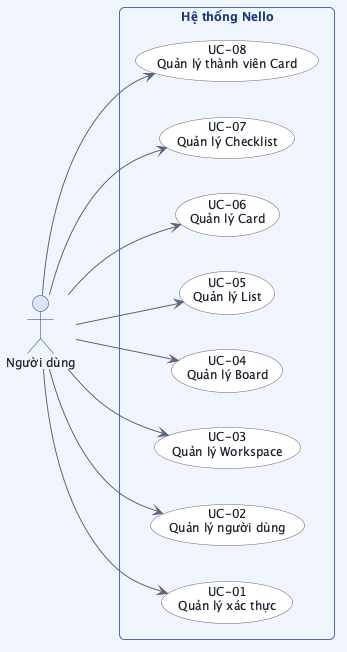
\includegraphics[width=0.75\textwidth]{images/chap3/usecase_overview.png}
\caption{Biểu đồ Use Case tổng quát hệ thống Nello}
\label{fig:usecase_overview}
\end{figure}

\paragraph{Phân rã Use Case} \mbox{}\\

Mỗi nhóm chức năng trong biểu đồ tổng quát được phân rã thành các use case thành phần cụ thể như sau:

\textbf{UC-01: Quản lý xác thực} -- Bao gồm đăng ký tài khoản, xác nhận OTP, gửi lại OTP, đăng nhập và làm mới access token.

\textbf{UC-02: Quản lý người dùng} -- Bao gồm xem thông tin cá nhân và chỉnh sửa thông tin cá nhân.

\textbf{UC-03: Quản lý Workspace} -- Bao gồm tạo, xem danh sách, xem chi tiết Workspace, mời thành viên và xem danh sách thành viên.

\textbf{UC-04: Quản lý Board} -- Bao gồm tạo, xem, cập nhật, xóa Board và thêm thành viên vào Board.

\textbf{UC-05: Quản lý List} -- Bao gồm tạo, đổi tên, xóa List và sắp xếp thứ tự List.

\textbf{UC-06: Quản lý Card} -- Bao gồm tạo, xem, cập nhật, đánh dấu hoàn thành, di chuyển và xóa Card.

\textbf{UC-07: Quản lý Checklist} -- Bao gồm tạo, cập nhật, xóa Checklist; tạo, cập nhật, đánh dấu hoàn thành và xóa Checklist Item.

\textbf{UC-08: Quản lý thành viên Card} -- Bao gồm gán và hủy gán thành viên vào Card.

\paragraph{Danh sách Use Case} \mbox{}\\

\begin{table}[H]
\centering
\begin{tabular}{|p{3cm}|p{11cm}|}
\hline
\textbf{Mã Use Case} & \textbf{Tên Use Case} \\
\hline
UC-01.1 & Đăng ký tài khoản \\
\hline
UC-01.2 & Xác nhận tài khoản bằng OTP \\
\hline
UC-01.3 & Gửi lại mã OTP \\
\hline
UC-01.4 & Đăng nhập \\
\hline
UC-01.5 & Làm mới access token \\
\hline
UC-02.1 & Xem thông tin cá nhân \\
\hline
UC-02.2 & Chỉnh sửa thông tin cá nhân \\
\hline
UC-03.1 & Tạo Workspace \\
\hline
UC-03.2 & Xem danh sách Workspace \\
\hline
UC-03.3 & Xem chi tiết Workspace \\
\hline
UC-03.4 & Mời thành viên vào Workspace \\
\hline
UC-03.5 & Xem danh sách thành viên Workspace \\
\hline
UC-04.1 & Tạo Board \\
\hline
UC-04.2 & Xem chi tiết Board \\
\hline
UC-04.3 & Cập nhật tên Board \\
\hline
UC-04.4 & Xóa Board \\
\hline
UC-04.5 & Thêm thành viên vào Board \\
\hline
UC-05.1 & Tạo List \\
\hline
UC-05.2 & Đổi tên List \\
\hline
UC-05.3 & Xóa List \\
\hline
UC-05.4 & Sắp xếp thứ tự List \\
\hline
UC-06.1 & Tạo Card \\
\hline
UC-06.2 & Xem chi tiết Card \\
\hline
UC-06.3 & Cập nhật Card \\
\hline
UC-06.4 & Đánh dấu Card hoàn thành \\
\hline
UC-06.5 & Di chuyển Card giữa các List \\
\hline
UC-06.6 & Xóa Card \\
\hline
UC-07.1 & Tạo Checklist \\
\hline
UC-07.2 & Cập nhật Checklist \\
\hline
UC-07.3 & Xóa Checklist \\
\hline
UC-07.4 & Tạo Checklist Item \\
\hline
UC-07.5 & Cập nhật Checklist Item \\
\hline
UC-07.6 & Đánh dấu Checklist Item hoàn thành \\
\hline
UC-07.7 & Xóa Checklist Item \\
\hline
UC-08.1 & Gán thành viên vào Card \\
\hline
UC-08.2 & Hủy gán thành viên khỏi Card \\
\hline
\end{tabular}
\caption{Danh sách Use Case}
\label{tab:usecase_list}
\end{table}

\subsubsection{Đặc tả Use Case}

\textbf{UC-01: Quản lý xác thực}

\begin{figure}[H]
\centering
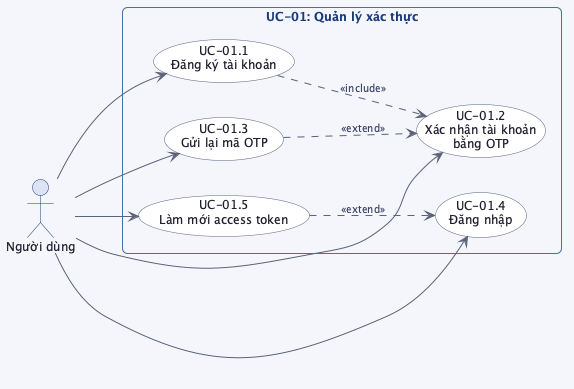
\includegraphics[width=\textwidth]{images/chap3/usecase_uc01.png}
\caption{Biểu đồ Use Case UC-01: Quản lý xác thực}
\label{fig:usecase_uc01}
\end{figure}

\vspace{0.3cm}
\noindent\begin{tabular}{|p{3.5cm}|p{10.5cm}|}
\hline
\textbf{Thành phần} & \textbf{Nội dung} \\
\hline
Mã Use Case & UC-01.1 \\
\hline
Tên Use Case & Đăng ký tài khoản \\
\hline
Tác nhân chính & Người dùng \\
\hline
Mô tả tóm tắt & Người dùng mới tạo tài khoản trong hệ thống thông qua Amazon Cognito. \\
\hline
Điều kiện & Người dùng chưa có tài khoản trong hệ thống. \\
\hline
Luồng chính & 1. Người dùng truy cập trang đăng ký.\newline 2. Hệ thống hiển thị form nhập họ tên, email và mật khẩu.\newline 3. Người dùng điền thông tin và nhấn Đăng ký.\newline 4. Hệ thống gọi Amazon Cognito tạo tài khoản.\newline 5. Cognito gửi mã OTP xác nhận về địa chỉ email.\newline 6. Nếu email đã tồn tại, hệ thống trả về lỗi HTTP 409. \\
\hline
Luồng thay thế & Email đã tồn tại: Hệ thống trả về lỗi HTTP 409.\newline Mật khẩu không đáp ứng yêu cầu bảo mật: Hệ thống hiển thị thông báo lỗi tại trường mật khẩu.\newline Lỗi kết nối Amazon Cognito: Hệ thống trả về lỗi HTTP 500. \\
\hline
\end{tabular}

\vspace{0.5cm}
\noindent\begin{tabular}{|p{3.5cm}|p{10.5cm}|}
\hline
\textbf{Thành phần} & \textbf{Nội dung} \\
\hline
Mã Use Case & UC-01.2 \\
\hline
Tên Use Case & Xác nhận tài khoản bằng OTP \\
\hline
Tác nhân chính & Người dùng \\
\hline
Mô tả tóm tắt & Người dùng nhập mã OTP nhận được qua email để kích hoạt tài khoản. \\
\hline
Điều kiện & Tài khoản đã được tạo; mã OTP đã được gửi về email. \\
\hline
Luồng chính & 1. Người dùng nhập mã OTP nhận được qua email.\newline 2. Người dùng nhấn Xác nhận.\newline 3. Hệ thống gửi yêu cầu xác nhận đến Amazon Cognito.\newline 4. Cognito kích hoạt tài khoản.\newline 5. Hệ thống chuyển hướng người dùng về trang đăng nhập.\newline 6. Nếu mã OTP sai hoặc hết hạn, hệ thống hiển thị thông báo lỗi. \\
\hline
Luồng thay thế & Mã OTP sai hoặc hết hạn: Hệ thống hiển thị thông báo lỗi, cho phép người dùng yêu cầu gửi lại mã.\newline Lỗi kết nối Amazon Cognito: Hệ thống trả về lỗi HTTP 500. \\
\hline
\end{tabular}

\vspace{0.5cm}
\noindent\begin{tabular}{|p{3.5cm}|p{10.5cm}|}
\hline
\textbf{Thành phần} & \textbf{Nội dung} \\
\hline
Mã Use Case & UC-01.3 \\
\hline
Tên Use Case & Gửi lại mã OTP \\
\hline
Tác nhân chính & Người dùng \\
\hline
Mô tả tóm tắt & Người dùng yêu cầu hệ thống gửi lại mã OTP khi mã cũ đã hết hạn hoặc chưa nhận được. \\
\hline
Điều kiện & Tài khoản đã đăng ký nhưng chưa xác nhận; mã OTP đã hết hạn hoặc chưa nhận được. \\
\hline
Luồng chính & 1. Người dùng nhấn Gửi lại mã OTP trên trang xác nhận.\newline 2. Hệ thống gọi Amazon Cognito để gửi lại mã OTP.\newline 3. Cognito gửi mã OTP mới về email.\newline 4. Hệ thống thông báo gửi lại thành công.\newline 5. Nếu quá số lần yêu cầu cho phép, hệ thống hiển thị thông báo lỗi. \\
\hline
Luồng thay thế & Vượt quá số lần yêu cầu gửi lại cho phép: Hệ thống hiển thị thông báo giới hạn và yêu cầu đợi.\newline Lỗi kết nối Amazon Cognito: Hệ thống trả về lỗi HTTP 500. \\
\hline
\end{tabular}

\vspace{0.5cm}
\noindent\begin{tabular}{|p{3.5cm}|p{10.5cm}|}
\hline
\textbf{Thành phần} & \textbf{Nội dung} \\
\hline
Mã Use Case & UC-01.4 \\
\hline
Tên Use Case & Đăng nhập \\
\hline
Tác nhân chính & Người dùng \\
\hline
Mô tả tóm tắt & Người dùng xác thực danh tính bằng email và mật khẩu để truy cập hệ thống. \\
\hline
Điều kiện & Người dùng đã có tài khoản và đã xác nhận email. \\
\hline
Luồng chính & 1. Người dùng truy cập trang đăng nhập.\newline 2. Hệ thống hiển thị form nhập email và mật khẩu.\newline 3. Người dùng nhập thông tin và nhấn Đăng nhập.\newline 4. Backend gọi Amazon Cognito để xác thực thông tin.\newline 5. Cognito trả về JWT (access token và refresh token).\newline 6. Backend lưu token vào HttpOnly cookie và chuyển hướng người dùng đến Dashboard.\newline 7. Nếu email hoặc mật khẩu sai, hệ thống hiển thị thông báo lỗi. \\
\hline
Luồng thay thế & Email hoặc mật khẩu không đúng: Hệ thống hiển thị thông báo lỗi xác thực.\newline Tài khoản chưa xác nhận email: Hệ thống yêu cầu xác nhận email trước khi đăng nhập.\newline Lỗi kết nối Amazon Cognito: Hệ thống trả về lỗi HTTP 500. \\
\hline
\end{tabular}

\vspace{0.5cm}
\noindent\begin{tabular}{|p{3.5cm}|p{10.5cm}|}
\hline
\textbf{Thành phần} & \textbf{Nội dung} \\
\hline
Mã Use Case & UC-01.5 \\
\hline
Tên Use Case & Làm mới access token \\
\hline
Tác nhân chính & Người dùng \\
\hline
Mô tả tóm tắt & Hệ thống tự động làm mới access token bằng refresh token khi token hết hạn. \\
\hline
Điều kiện & Người dùng đã đăng nhập; access token đã hết hạn; refresh token còn hiệu lực. \\
\hline
Luồng chính & 1. Hệ thống phát hiện access token hết hạn khi xử lý request.\newline 2. Hệ thống sử dụng refresh token trong HttpOnly cookie để gọi endpoint làm mới token.\newline 3. Backend gọi Amazon Cognito để cấp access token mới.\newline 4. Backend cập nhật HttpOnly cookie với access token mới.\newline 5. Request gốc của người dùng được thực hiện lại.\newline 6. Nếu refresh token hết hạn, hệ thống yêu cầu người dùng đăng nhập lại. \\
\hline
Luồng thay thế & Refresh token đã hết hạn: Hệ thống xóa cookie và yêu cầu người dùng đăng nhập lại.\newline Lỗi kết nối Amazon Cognito: Hệ thống trả về lỗi HTTP 500. \\
\hline
\end{tabular}

\vspace{0.5cm}

\textbf{UC-02: Quản lý người dùng}

\begin{figure}[H]
\centering
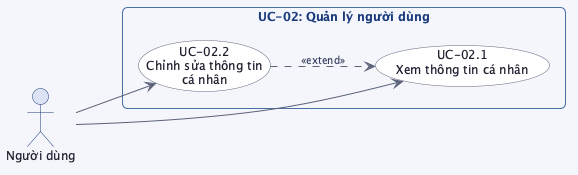
\includegraphics[width=\textwidth]{images/chap3/usecase_uc02.png}
\caption{Biểu đồ Use Case UC-02: Quản lý người dùng}
\label{fig:usecase_uc02}
\end{figure}

\vspace{0.3cm}
\noindent\begin{tabular}{|p{3.5cm}|p{10.5cm}|}
\hline
\textbf{Thành phần} & \textbf{Nội dung} \\
\hline
Mã Use Case & UC-02.1 \\
\hline
Tên Use Case & Xem thông tin cá nhân \\
\hline
Tác nhân chính & Người dùng \\
\hline
Mô tả tóm tắt & Người dùng xem thông tin hồ sơ cá nhân của mình trong hệ thống. \\
\hline
Điều kiện & Người dùng đã đăng nhập thành công. \\
\hline
Luồng chính & 1. Người dùng truy cập trang thông tin cá nhân.\newline 2. Hệ thống gọi API GET /api/v1/users/me với access token.\newline 3. Backend trích xuất thông tin người dùng từ JWT và truy vấn cơ sở dữ liệu.\newline 4. Hệ thống hiển thị họ tên, email, ảnh đại diện và các thông tin cá nhân khác. \\
\hline
Luồng thay thế & Access token không hợp lệ hoặc hết hạn: Hệ thống chuyển hướng về trang đăng nhập.\newline Lỗi truy vấn cơ sở dữ liệu: Hệ thống trả về lỗi HTTP 500. \\
\hline
\end{tabular}

\vspace{0.5cm}
\noindent\begin{tabular}{|p{3.5cm}|p{10.5cm}|}
\hline
\textbf{Thành phần} & \textbf{Nội dung} \\
\hline
Mã Use Case & UC-02.2 \\
\hline
Tên Use Case & Chỉnh sửa thông tin cá nhân \\
\hline
Tác nhân chính & Người dùng \\
\hline
Mô tả tóm tắt & Người dùng cập nhật các thông tin cá nhân như họ tên, ảnh đại diện, số điện thoại và địa chỉ. \\
\hline
Điều kiện & Người dùng đã đăng nhập và đang ở trang thông tin cá nhân. \\
\hline
Luồng chính & 1. Người dùng truy cập trang thông tin cá nhân.\newline 2. Người dùng chọn chỉnh sửa và thay đổi các trường thông tin.\newline 3. Người dùng xác nhận lưu.\newline 4. Hệ thống gọi API cập nhật và lưu thông tin mới vào cơ sở dữ liệu.\newline 5. Hệ thống hiển thị thông báo cập nhật thành công. \\
\hline
Luồng thay thế & Thông tin nhập không hợp lệ (họ tên bị bỏ trống): Hệ thống hiển thị thông báo lỗi và yêu cầu nhập lại. \\
\hline
\end{tabular}

\vspace{0.5cm}

\textbf{UC-03: Quản lý Workspace}

\begin{figure}[H]
\centering
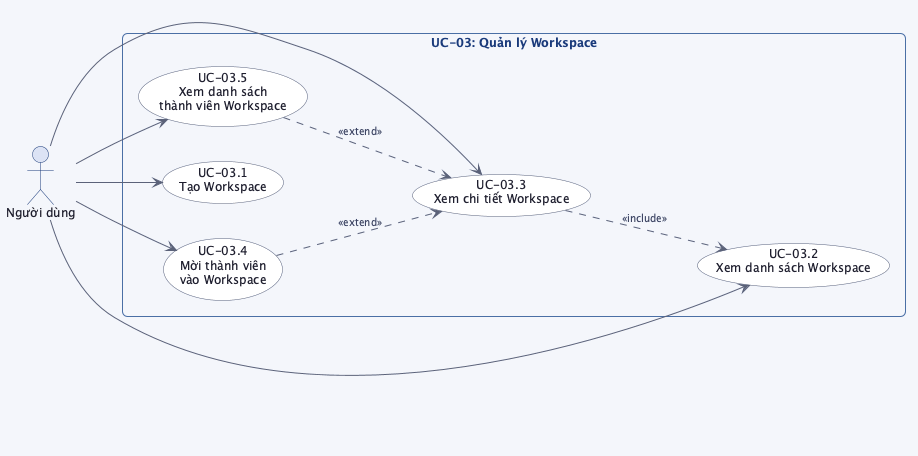
\includegraphics[width=\textwidth]{images/chap3/usecase_uc03.png}
\caption{Biểu đồ Use Case UC-03: Quản lý Workspace}
\label{fig:usecase_uc03}
\end{figure}

\vspace{0.3cm}
\noindent\begin{tabular}{|p{3.5cm}|p{10.5cm}|}
\hline
\textbf{Thành phần} & \textbf{Nội dung} \\
\hline
Mã Use Case & UC-03.1 \\
\hline
Tên Use Case & Tạo Workspace \\
\hline
Tác nhân chính & Người dùng \\
\hline
Mô tả tóm tắt & Người dùng tạo không gian làm việc mới để quản lý các Board liên quan. \\
\hline
Điều kiện & Người dùng đã đăng nhập thành công. \\
\hline
Luồng chính & 1. Người dùng chọn chức năng tạo Workspace.\newline 2. Hệ thống hiển thị form nhập tên, loại và mô tả Workspace.\newline 3. Người dùng điền thông tin và nhấn Tạo.\newline 4. Hệ thống gọi API POST /api/v1/workspaces.\newline 5. Backend tạo Workspace và tự động thêm người tạo làm thành viên với vai trò ADMIN.\newline 6. Hệ thống hiển thị Workspace mới trong danh sách.\newline 7. Nếu tên Workspace bị bỏ trống, hệ thống trả về lỗi HTTP 400. \\
\hline
Luồng thay thế & Tên Workspace bị bỏ trống: Hệ thống trả về lỗi HTTP 400.\newline Lỗi không xác định: Hệ thống trả về lỗi HTTP 500. \\
\hline
\end{tabular}

\vspace{0.5cm}
\noindent\begin{tabular}{|p{3.5cm}|p{10.5cm}|}
\hline
\textbf{Thành phần} & \textbf{Nội dung} \\
\hline
Mã Use Case & UC-03.2 \\
\hline
Tên Use Case & Xem danh sách Workspace \\
\hline
Tác nhân chính & Người dùng \\
\hline
Mô tả tóm tắt & Người dùng xem toàn bộ danh sách Workspace mà mình sở hữu hoặc là thành viên. \\
\hline
Điều kiện & Người dùng đã đăng nhập thành công. \\
\hline
Luồng chính & 1. Người dùng truy cập trang Dashboard.\newline 2. Hệ thống gọi API GET /api/v1/workspaces.\newline 3. Backend truy vấn danh sách Workspace mà người dùng sở hữu hoặc là thành viên.\newline 4. Hệ thống hiển thị danh sách Workspace kèm tên và mô tả. \\
\hline
Luồng thay thế & Người dùng chưa có Workspace nào: Hệ thống hiển thị giao diện trống kèm gợi ý tạo Workspace mới. \\
\hline
\end{tabular}

\vspace{0.5cm}
\noindent\begin{tabular}{|p{3.5cm}|p{10.5cm}|}
\hline
\textbf{Thành phần} & \textbf{Nội dung} \\
\hline
Mã Use Case & UC-03.3 \\
\hline
Tên Use Case & Xem chi tiết Workspace \\
\hline
Tác nhân chính & Người dùng \\
\hline
Mô tả tóm tắt & Người dùng xem thông tin chi tiết và danh sách Board trong một Workspace. \\
\hline
Điều kiện & Người dùng đã đăng nhập và là thành viên của Workspace. \\
\hline
Luồng chính & 1. Người dùng chọn một Workspace từ danh sách.\newline 2. Hệ thống gọi API GET /api/v1/workspaces/:id.\newline 3. Backend kiểm tra quyền truy cập của người dùng.\newline 4. Hệ thống hiển thị tên, mô tả, loại Workspace và danh sách Board bên trong.\newline 5. Nếu Workspace không tồn tại hoặc người dùng không có quyền, hệ thống trả về lỗi HTTP 404 hoặc HTTP 403. \\
\hline
Luồng thay thế & Workspace không tồn tại: Hệ thống trả về lỗi HTTP 404.\newline Người dùng không có quyền truy cập: Hệ thống trả về lỗi HTTP 403. \\
\hline
\end{tabular}

\vspace{0.5cm}
\noindent\begin{tabular}{|p{3.5cm}|p{10.5cm}|}
\hline
\textbf{Thành phần} & \textbf{Nội dung} \\
\hline
Mã Use Case & UC-03.4 \\
\hline
Tên Use Case & Mời thành viên vào Workspace \\
\hline
Tác nhân chính & Người dùng \\
\hline
Mô tả tóm tắt & Người dùng có vai trò ADMIN mời người dùng khác tham gia vào Workspace. \\
\hline
Điều kiện & Người dùng đã đăng nhập và có vai trò ADMIN trong Workspace. \\
\hline
Luồng chính & 1. Người dùng truy cập trang quản lý thành viên Workspace.\newline 2. Người dùng tìm kiếm thành viên cần mời theo email.\newline 3. Người dùng chọn thành viên từ kết quả tìm kiếm và nhấn Mời.\newline 4. Hệ thống gọi API POST /api/v1/workspaces-members/:workspaceId.\newline 5. Backend kiểm tra người dùng tồn tại và chưa là thành viên.\newline 6. Backend thêm người dùng vào Workspace với vai trò MEMBER.\newline 7. Hệ thống cập nhật danh sách thành viên.\newline 8. Nếu người dùng đã là thành viên, hệ thống hiển thị thông báo lỗi. \\
\hline
Luồng thay thế & Người dùng được mời không tồn tại trong hệ thống: Hệ thống hiển thị thông báo lỗi.\newline Người dùng đã là thành viên của Workspace: Hệ thống hiển thị thông báo trùng lặp.\newline Người dùng không có quyền ADMIN: Hệ thống trả về lỗi HTTP 403. \\
\hline
\end{tabular}

\vspace{0.5cm}
\noindent\begin{tabular}{|p{3.5cm}|p{10.5cm}|}
\hline
\textbf{Thành phần} & \textbf{Nội dung} \\
\hline
Mã Use Case & UC-03.5 \\
\hline
Tên Use Case & Xem danh sách thành viên Workspace \\
\hline
Tác nhân chính & Người dùng \\
\hline
Mô tả tóm tắt & Người dùng xem danh sách các thành viên hiện có trong Workspace cùng vai trò của từng người. \\
\hline
Điều kiện & Người dùng đã đăng nhập và là thành viên của Workspace. \\
\hline
Luồng chính & 1. Người dùng truy cập trang thành viên của Workspace.\newline 2. Hệ thống gọi API GET /api/v1/workspaces/:id/members.\newline 3. Backend truy vấn danh sách thành viên cùng vai trò trong Workspace.\newline 4. Hệ thống hiển thị danh sách thành viên kèm tên, email và vai trò. \\
\hline
Luồng thay thế & Workspace không tồn tại: Hệ thống trả về lỗi HTTP 404.\newline Người dùng không có quyền truy cập: Hệ thống trả về lỗi HTTP 403. \\
\hline
\end{tabular}

\vspace{0.5cm}

\textbf{UC-04: Quản lý Board}

\begin{figure}[H]
\centering
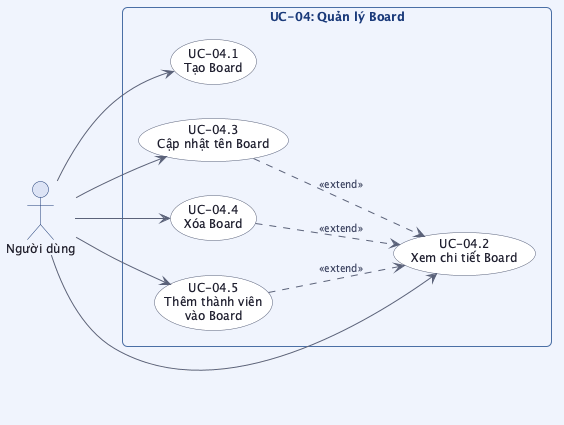
\includegraphics[width=\textwidth]{images/chap3/usecase_uc04.png}
\caption{Biểu đồ Use Case UC-04: Quản lý Board}
\label{fig:usecase_uc04}
\end{figure}

\vspace{0.3cm}
\noindent\begin{tabular}{|p{3.5cm}|p{10.5cm}|}
\hline
\textbf{Thành phần} & \textbf{Nội dung} \\
\hline
Mã Use Case & UC-04.1 \\
\hline
Tên Use Case & Tạo Board \\
\hline
Tác nhân chính & Người dùng \\
\hline
Mô tả tóm tắt & Người dùng tạo bảng công việc mới trong Workspace để quản lý các List và Card theo mô hình Kanban. \\
\hline
Điều kiện & Người dùng đã đăng nhập và có vai trò ADMIN trong Workspace. \\
\hline
Luồng chính & 1. Người dùng chọn chức năng tạo Board trong Workspace.\newline 2. Hệ thống hiển thị form nhập tên và chọn hình nền Board.\newline 3. Người dùng điền tên, chọn hình nền và nhấn Tạo.\newline 4. Hệ thống gọi API POST /api/v1/boards với workspaceId, title và backgroundUrl.\newline 5. Backend kiểm tra quyền ADMIN của người dùng trong Workspace.\newline 6. Backend tạo Board và trả về thông tin Board mới.\newline 7. Hệ thống hiển thị Board mới trong danh sách Workspace.\newline 8. Nếu người dùng không có quyền ADMIN, hệ thống trả về lỗi HTTP 403. \\
\hline
Luồng thay thế & Người dùng không có quyền ADMIN trong Workspace: Hệ thống trả về lỗi HTTP 403.\newline Tên Board bị bỏ trống: Hệ thống trả về lỗi HTTP 400. \\
\hline
\end{tabular}

\vspace{0.5cm}
\noindent\begin{tabular}{|p{3.5cm}|p{10.5cm}|}
\hline
\textbf{Thành phần} & \textbf{Nội dung} \\
\hline
Mã Use Case & UC-04.2 \\
\hline
Tên Use Case & Xem chi tiết Board \\
\hline
Tác nhân chính & Người dùng \\
\hline
Mô tả tóm tắt & Người dùng tải và xem toàn bộ nội dung Board bao gồm danh sách List và Card theo mô hình Kanban. \\
\hline
Điều kiện & Người dùng đã đăng nhập và là thành viên của Board. \\
\hline
Luồng chính & 1. Người dùng chọn Board từ danh sách.\newline 2. Hệ thống gọi API GET /api/v1/boards/:id.\newline 3. Backend kiểm tra quyền của người dùng trong Board.\newline 4. Hệ thống tải và hiển thị toàn bộ List và Card theo mô hình Kanban.\newline 5. Nếu Board không tồn tại hoặc người dùng không có quyền, hệ thống trả về lỗi HTTP 404 hoặc HTTP 403. \\
\hline
Luồng thay thế & Board không tồn tại: Hệ thống trả về lỗi HTTP 404.\newline Người dùng không có quyền truy cập Board: Hệ thống trả về lỗi HTTP 403. \\
\hline
\end{tabular}

\vspace{0.5cm}
\noindent\begin{tabular}{|p{3.5cm}|p{10.5cm}|}
\hline
\textbf{Thành phần} & \textbf{Nội dung} \\
\hline
Mã Use Case & UC-04.3 \\
\hline
Tên Use Case & Cập nhật tên Board \\
\hline
Tác nhân chính & Người dùng \\
\hline
Mô tả tóm tắt & Người dùng thay đổi tên của Board. \\
\hline
Điều kiện & Người dùng đã đăng nhập và có vai trò ADMIN trong Board. \\
\hline
Luồng chính & 1. Người dùng chọn chỉnh sửa tên Board.\newline 2. Hệ thống hiển thị ô nhập tên mới.\newline 3. Người dùng nhập tên mới và xác nhận.\newline 4. Hệ thống gọi API PUT /api/v1/boards/:id với tên mới.\newline 5. Backend cập nhật tên Board trong cơ sở dữ liệu.\newline 6. Hệ thống hiển thị tên Board đã cập nhật. \\
\hline
Luồng thay thế & Tên mới bị bỏ trống: Hệ thống không cho phép cập nhật.\newline Người dùng không có quyền ADMIN: Hệ thống trả về lỗi HTTP 403. \\
\hline
\end{tabular}

\vspace{0.5cm}
\noindent\begin{tabular}{|p{3.5cm}|p{10.5cm}|}
\hline
\textbf{Thành phần} & \textbf{Nội dung} \\
\hline
Mã Use Case & UC-04.4 \\
\hline
Tên Use Case & Xóa Board \\
\hline
Tác nhân chính & Người dùng \\
\hline
Mô tả tóm tắt & Người dùng xóa vĩnh viễn Board cùng toàn bộ List và Card bên trong. \\
\hline
Điều kiện & Người dùng đã đăng nhập và có vai trò ADMIN trong Board. \\
\hline
Luồng chính & 1. Người dùng chọn xóa Board.\newline 2. Hệ thống hiển thị hộp thoại xác nhận xóa.\newline 3. Người dùng xác nhận thao tác.\newline 4. Hệ thống gọi API DELETE /api/v1/boards/:id.\newline 5. Backend xóa Board và toàn bộ List, Card bên trong theo cơ chế cascade delete.\newline 6. Hệ thống chuyển hướng người dùng về trang Workspace.\newline 7. Nếu người dùng không có quyền ADMIN, hệ thống trả về lỗi HTTP 403. \\
\hline
Luồng thay thế & Người dùng không có quyền ADMIN trong Board: Hệ thống trả về lỗi HTTP 403.\newline Board không tồn tại: Hệ thống trả về lỗi HTTP 404. \\
\hline
\end{tabular}

\vspace{0.5cm}
\noindent\begin{tabular}{|p{3.5cm}|p{10.5cm}|}
\hline
\textbf{Thành phần} & \textbf{Nội dung} \\
\hline
Mã Use Case & UC-04.5 \\
\hline
Tên Use Case & Thêm thành viên vào Board \\
\hline
Tác nhân chính & Người dùng \\
\hline
Mô tả tóm tắt & Người dùng có vai trò ADMIN thêm thành viên từ Workspace vào Board với vai trò nhất định. \\
\hline
Điều kiện & Người dùng đã đăng nhập và có vai trò ADMIN trong Board; thành viên cần thêm phải là thành viên của Workspace. \\
\hline
Luồng chính & 1. Người dùng truy cập trang quản lý thành viên Board.\newline 2. Người dùng tìm kiếm thành viên trong Workspace và chọn người cần thêm.\newline 3. Người dùng chọn vai trò (ADMIN, MEMBER hoặc VIEWER) và nhấn Thêm.\newline 4. Hệ thống gọi API POST /api/v1/boards-members với userIds, boardId và roleId.\newline 5. Backend kiểm tra thành viên thuộc Workspace và chưa có trong Board.\newline 6. Backend thêm thành viên vào Board với vai trò được chỉ định.\newline 7. Hệ thống cập nhật danh sách thành viên Board. \\
\hline
Luồng thay thế & Thành viên không thuộc Workspace: Hệ thống không cho phép thêm vào Board.\newline Thành viên đã có trong Board: Hệ thống hiển thị thông báo trùng lặp.\newline Người dùng không có quyền ADMIN: Hệ thống trả về lỗi HTTP 403. \\
\hline
\end{tabular}

\vspace{0.5cm}

\textbf{UC-05: Quản lý List}

\begin{figure}[H]
\centering
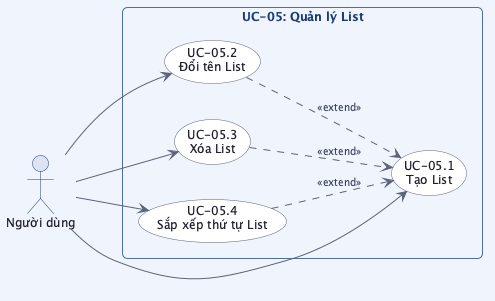
\includegraphics[width=\textwidth]{images/chap3/usecase_uc05.png}
\caption{Biểu đồ Use Case UC-05: Quản lý List}
\label{fig:usecase_uc05}
\end{figure}

\vspace{0.3cm}
\noindent\begin{tabular}{|p{3.5cm}|p{10.5cm}|}
\hline
\textbf{Thành phần} & \textbf{Nội dung} \\
\hline
Mã Use Case & UC-05.1 \\
\hline
Tên Use Case & Tạo List \\
\hline
Tác nhân chính & Người dùng \\
\hline
Mô tả tóm tắt & Người dùng tạo cột danh sách công việc mới trong Board. \\
\hline
Điều kiện & Người dùng đã đăng nhập và là thành viên của Board. \\
\hline
Luồng chính & 1. Người dùng chọn thêm List mới trong Board.\newline 2. Hệ thống hiển thị ô nhập tên List.\newline 3. Người dùng nhập tên và nhấn Thêm.\newline 4. Hệ thống gọi API POST /api/v1/lists với boardId và title.\newline 5. Backend tạo List mới và trả về listId, title, boardId.\newline 6. Hệ thống hiển thị List mới ở cuối Board.\newline 7. Nếu tên bị bỏ trống, hệ thống không cho phép tạo. \\
\hline
Luồng thay thế & Tên List bị bỏ trống: Hệ thống không cho phép tạo.\newline Board không tồn tại: Hệ thống trả về lỗi HTTP 404. \\
\hline
\end{tabular}

\vspace{0.5cm}
\noindent\begin{tabular}{|p{3.5cm}|p{10.5cm}|}
\hline
\textbf{Thành phần} & \textbf{Nội dung} \\
\hline
Mã Use Case & UC-05.2 \\
\hline
Tên Use Case & Đổi tên List \\
\hline
Tác nhân chính & Người dùng \\
\hline
Mô tả tóm tắt & Người dùng thay đổi tên của một List trong Board. \\
\hline
Điều kiện & Người dùng đã đăng nhập và là thành viên của Board. \\
\hline
Luồng chính & 1. Người dùng nhấp vào tên List hiện tại.\newline 2. Hệ thống chuyển sang chế độ chỉnh sửa tên.\newline 3. Người dùng nhập tên mới và xác nhận.\newline 4. Hệ thống gọi API PATCH /api/v1/lists/:id với tên mới.\newline 5. Backend cập nhật tên List trong cơ sở dữ liệu.\newline 6. Hệ thống hiển thị tên List đã cập nhật. \\
\hline
Luồng thay thế & Tên mới bị bỏ trống: Hệ thống không cho phép cập nhật.\newline List không tồn tại: Hệ thống trả về lỗi HTTP 404. \\
\hline
\end{tabular}

\vspace{0.5cm}
\noindent\begin{tabular}{|p{3.5cm}|p{10.5cm}|}
\hline
\textbf{Thành phần} & \textbf{Nội dung} \\
\hline
Mã Use Case & UC-05.3 \\
\hline
Tên Use Case & Xóa List \\
\hline
Tác nhân chính & Người dùng \\
\hline
Mô tả tóm tắt & Người dùng xóa List và toàn bộ Card bên trong. \\
\hline
Điều kiện & Người dùng đã đăng nhập và là thành viên của Board. \\
\hline
Luồng chính & 1. Người dùng chọn xóa List.\newline 2. Hệ thống hiển thị hộp thoại xác nhận.\newline 3. Người dùng xác nhận thao tác.\newline 4. Hệ thống gọi API DELETE /api/v1/lists/:id.\newline 5. Backend xóa List và toàn bộ Card bên trong theo cơ chế cascade delete.\newline 6. Hệ thống cập nhật giao diện Board. \\
\hline
Luồng thay thế & List không tồn tại: Hệ thống trả về lỗi HTTP 404. \\
\hline
\end{tabular}

\vspace{0.5cm}
\noindent\begin{tabular}{|p{3.5cm}|p{10.5cm}|}
\hline
\textbf{Thành phần} & \textbf{Nội dung} \\
\hline
Mã Use Case & UC-05.4 \\
\hline
Tên Use Case & Sắp xếp thứ tự List \\
\hline
Tác nhân chính & Người dùng \\
\hline
Mô tả tóm tắt & Người dùng kéo thả để thay đổi thứ tự hiển thị của các List trong Board. \\
\hline
Điều kiện & Người dùng đã đăng nhập và là thành viên của Board. \\
\hline
Luồng chính & 1. Người dùng nhấn giữ và kéo List sang vị trí mong muốn.\newline 2. Frontend tính toán giá trị position mới dựa trên thuật toán fractional indexing.\newline 3. Giao diện cập nhật thứ tự List ngay lập tức (optimistic update).\newline 4. Hệ thống gọi API PATCH /api/v1/lists/:id với position mới.\newline 5. Backend cập nhật trường position trong cơ sở dữ liệu. \\
\hline
Luồng thay thế & Lỗi xảy ra khi cập nhật position: Hệ thống hoàn tác về thứ tự cũ và hiển thị thông báo lỗi. \\
\hline
\end{tabular}

\vspace{0.5cm}

\textbf{UC-06: Quản lý Card}

\begin{figure}[H]
\centering
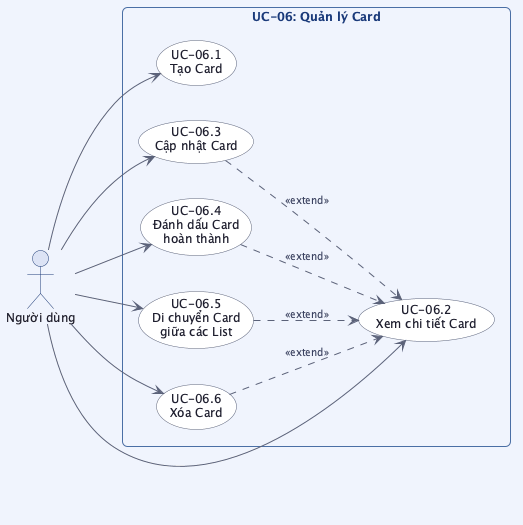
\includegraphics[width=\textwidth]{images/chap3/usecase_uc06.png}
\caption{Biểu đồ Use Case UC-06: Quản lý Card}
\label{fig:usecase_uc06}
\end{figure}

\vspace{0.3cm}
\noindent\begin{tabular}{|p{3.5cm}|p{10.5cm}|}
\hline
\textbf{Thành phần} & \textbf{Nội dung} \\
\hline
Mã Use Case & UC-06.1 \\
\hline
Tên Use Case & Tạo Card \\
\hline
Tác nhân chính & Người dùng \\
\hline
Mô tả tóm tắt & Người dùng tạo thẻ công việc mới trong một List. \\
\hline
Điều kiện & Người dùng đã đăng nhập và là thành viên của Board. \\
\hline
Luồng chính & 1. Người dùng chọn thêm Card trong một List.\newline 2. Hệ thống hiển thị ô nhập tiêu đề Card.\newline 3. Người dùng nhập tiêu đề và nhấn Thêm.\newline 4. Hệ thống gọi API POST /api/v1/cards với listId, title và position.\newline 5. Backend kiểm tra quyền người dùng trong Board.\newline 6. Backend tạo Card và trả về cardId, title, listId, position.\newline 7. Hệ thống hiển thị Card mới ở cuối List. \\
\hline
Luồng thay thế & Tiêu đề Card bị bỏ trống: Hệ thống không cho phép tạo.\newline List không tồn tại: Hệ thống trả về lỗi HTTP 404.\newline Người dùng không có quyền trong Board: Hệ thống trả về lỗi HTTP 403. \\
\hline
\end{tabular}

\vspace{0.5cm}
\noindent\begin{tabular}{|p{3.5cm}|p{10.5cm}|}
\hline
\textbf{Thành phần} & \textbf{Nội dung} \\
\hline
Mã Use Case & UC-06.2 \\
\hline
Tên Use Case & Xem chi tiết Card \\
\hline
Tác nhân chính & Người dùng \\
\hline
Mô tả tóm tắt & Người dùng xem đầy đủ thông tin chi tiết của một Card bao gồm mô tả, ngày tháng, thành viên và checklist. \\
\hline
Điều kiện & Người dùng đã đăng nhập và là thành viên của Board. \\
\hline
Luồng chính & 1. Người dùng nhấp vào Card.\newline 2. Hệ thống gọi API GET /api/v1/cards/:id.\newline 3. Backend trả về đầy đủ thông tin Card bao gồm tiêu đề, mô tả, ngày bắt đầu, ngày đến hạn, trạng thái hoàn thành, thành viên phụ trách và danh sách Checklist.\newline 4. Hệ thống hiển thị modal chi tiết Card. \\
\hline
Luồng thay thế & Card không tồn tại: Hệ thống trả về lỗi HTTP 404.\newline Người dùng không có quyền trong Board: Hệ thống trả về lỗi HTTP 403. \\
\hline
\end{tabular}

\vspace{0.5cm}
\noindent\begin{tabular}{|p{3.5cm}|p{10.5cm}|}
\hline
\textbf{Thành phần} & \textbf{Nội dung} \\
\hline
Mã Use Case & UC-06.3 \\
\hline
Tên Use Case & Cập nhật Card \\
\hline
Tác nhân chính & Người dùng \\
\hline
Mô tả tóm tắt & Người dùng chỉnh sửa thông tin của Card bao gồm tiêu đề, mô tả, ngày bắt đầu và ngày đến hạn. \\
\hline
Điều kiện & Người dùng đã đăng nhập và là thành viên của Board. \\
\hline
Luồng chính & 1. Người dùng mở modal chi tiết Card.\newline 2. Người dùng chỉnh sửa các trường thông tin cần thiết (tiêu đề, mô tả, ngày bắt đầu, ngày đến hạn).\newline 3. Hệ thống gọi API PATCH /api/v1/cards/:id với các trường đã thay đổi.\newline 4. Backend cập nhật Card trong cơ sở dữ liệu.\newline 5. Hệ thống hiển thị thông tin Card đã cập nhật. \\
\hline
Luồng thay thế & Tiêu đề bị bỏ trống: Hệ thống không cho phép lưu.\newline Lỗi không xác định: Hệ thống trả về lỗi HTTP 500. \\
\hline
\end{tabular}

\vspace{0.5cm}
\noindent\begin{tabular}{|p{3.5cm}|p{10.5cm}|}
\hline
\textbf{Thành phần} & \textbf{Nội dung} \\
\hline
Mã Use Case & UC-06.4 \\
\hline
Tên Use Case & Đánh dấu Card hoàn thành \\
\hline
Tác nhân chính & Người dùng \\
\hline
Mô tả tóm tắt & Người dùng cập nhật trạng thái hoàn thành của Card. \\
\hline
Điều kiện & Người dùng đã đăng nhập và là thành viên của Board. \\
\hline
Luồng chính & 1. Người dùng mở modal chi tiết Card.\newline 2. Người dùng tích vào ô đánh dấu hoàn thành.\newline 3. Hệ thống gọi API PATCH /api/v1/cards/:id với isCompleted = true.\newline 4. Backend cập nhật trạng thái hoàn thành trong cơ sở dữ liệu.\newline 5. Hệ thống hiển thị trạng thái hoàn thành trên Card và trong modal. \\
\hline
Luồng thay thế & Lỗi xảy ra khi cập nhật: Hệ thống hoàn tác về trạng thái cũ và hiển thị thông báo lỗi. \\
\hline
\end{tabular}

\vspace{0.5cm}
\noindent\begin{tabular}{|p{3.5cm}|p{10.5cm}|}
\hline
\textbf{Thành phần} & \textbf{Nội dung} \\
\hline
Mã Use Case & UC-06.5 \\
\hline
Tên Use Case & Di chuyển Card giữa các List \\
\hline
Tác nhân chính & Người dùng \\
\hline
Mô tả tóm tắt & Người dùng kéo thả Card sang List khác hoặc thay đổi vị trí trong cùng một List. \\
\hline
Điều kiện & Người dùng đã đăng nhập và là thành viên của Board. \\
\hline
Luồng chính & 1. Người dùng nhấn giữ và kéo Card sang List mới hoặc vị trí khác trong cùng List.\newline 2. Frontend tính toán listId đích và giá trị position mới.\newline 3. Giao diện cập nhật vị trí Card ngay lập tức (optimistic update).\newline 4. Hệ thống gọi API PATCH /api/v1/cards/:id với listId mới và position mới.\newline 5. Backend cập nhật listId và position của Card trong cơ sở dữ liệu. \\
\hline
Luồng thay thế & Lỗi xảy ra khi cập nhật position: Hệ thống hoàn tác Card về vị trí cũ và hiển thị thông báo lỗi. \\
\hline
\end{tabular}

\vspace{0.5cm}
\noindent\begin{tabular}{|p{3.5cm}|p{10.5cm}|}
\hline
\textbf{Thành phần} & \textbf{Nội dung} \\
\hline
Mã Use Case & UC-06.6 \\
\hline
Tên Use Case & Xóa Card \\
\hline
Tác nhân chính & Người dùng \\
\hline
Mô tả tóm tắt & Người dùng xóa Card và toàn bộ Checklist, ChecklistItem, CardMember liên quan. \\
\hline
Điều kiện & Người dùng đã đăng nhập và là thành viên của Board. \\
\hline
Luồng chính & 1. Người dùng mở modal chi tiết Card và chọn xóa.\newline 2. Hệ thống hiển thị hộp thoại xác nhận.\newline 3. Người dùng xác nhận thao tác.\newline 4. Hệ thống gọi API DELETE /api/v1/cards/:id.\newline 5. Backend xóa Card và toàn bộ dữ liệu liên quan theo cơ chế cascade delete.\newline 6. Hệ thống đóng modal và cập nhật giao diện Board. \\
\hline
Luồng thay thế & Card không tồn tại: Hệ thống trả về lỗi HTTP 404.\newline Lỗi không xác định: Hệ thống trả về lỗi HTTP 500. \\
\hline
\end{tabular}

\vspace{0.5cm}

\textbf{UC-07: Quản lý Checklist}

\begin{figure}[H]
\centering
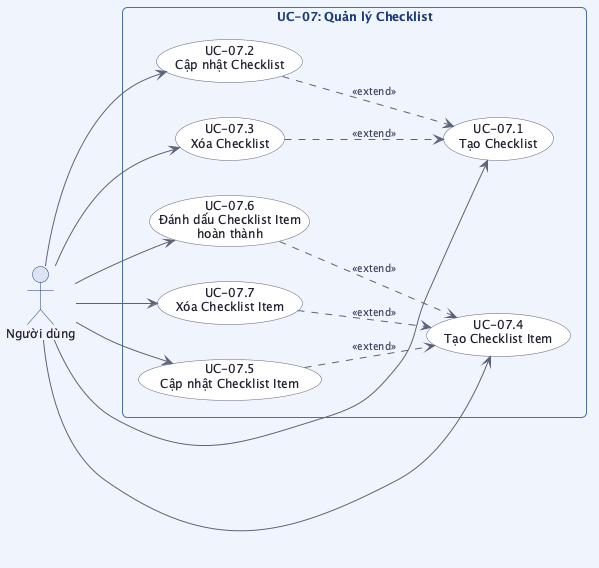
\includegraphics[width=\textwidth]{images/chap3/usecase_uc07.png}
\caption{Biểu đồ Use Case UC-07: Quản lý Checklist}
\label{fig:usecase_uc07}
\end{figure}

\vspace{0.3cm}
\noindent\begin{tabular}{|p{3.5cm}|p{10.5cm}|}
\hline
\textbf{Thành phần} & \textbf{Nội dung} \\
\hline
Mã Use Case & UC-07.1 \\
\hline
Tên Use Case & Tạo Checklist \\
\hline
Tác nhân chính & Người dùng \\
\hline
Mô tả tóm tắt & Người dùng tạo danh sách kiểm tra mới bên trong một Card. \\
\hline
Điều kiện & Người dùng đã đăng nhập và là thành viên của Board; Card đang mở. \\
\hline
Luồng chính & 1. Người dùng chọn thêm Checklist trong modal Card.\newline 2. Hệ thống hiển thị ô nhập tên Checklist.\newline 3. Người dùng nhập tên và nhấn Thêm.\newline 4. Hệ thống gọi API POST /api/v1/checklists với cardId, name và position.\newline 5. Backend tạo Checklist và trả về thông tin.\newline 6. Hệ thống hiển thị Checklist mới trong modal Card. \\
\hline
Luồng thay thế & Tên Checklist bị bỏ trống: Hệ thống không cho phép tạo.\newline Card không tồn tại: Hệ thống trả về lỗi HTTP 404. \\
\hline
\end{tabular}

\vspace{0.5cm}
\noindent\begin{tabular}{|p{3.5cm}|p{10.5cm}|}
\hline
\textbf{Thành phần} & \textbf{Nội dung} \\
\hline
Mã Use Case & UC-07.2 \\
\hline
Tên Use Case & Cập nhật Checklist \\
\hline
Tác nhân chính & Người dùng \\
\hline
Mô tả tóm tắt & Người dùng thay đổi tên của Checklist. \\
\hline
Điều kiện & Người dùng đã đăng nhập và là thành viên của Board; Checklist tồn tại. \\
\hline
Luồng chính & 1. Người dùng nhấp vào tên Checklist để chỉnh sửa.\newline 2. Người dùng nhập tên mới và xác nhận.\newline 3. Hệ thống gọi API PATCH /api/v1/checklists/:id với tên mới.\newline 4. Backend cập nhật tên Checklist trong cơ sở dữ liệu.\newline 5. Hệ thống hiển thị tên Checklist đã cập nhật. \\
\hline
Luồng thay thế & Tên mới bị bỏ trống: Hệ thống không cho phép cập nhật.\newline Checklist không tồn tại: Hệ thống trả về lỗi HTTP 404. \\
\hline
\end{tabular}

\vspace{0.5cm}
\noindent\begin{tabular}{|p{3.5cm}|p{10.5cm}|}
\hline
\textbf{Thành phần} & \textbf{Nội dung} \\
\hline
Mã Use Case & UC-07.3 \\
\hline
Tên Use Case & Xóa Checklist \\
\hline
Tác nhân chính & Người dùng \\
\hline
Mô tả tóm tắt & Người dùng xóa Checklist và toàn bộ ChecklistItem bên trong. \\
\hline
Điều kiện & Người dùng đã đăng nhập và là thành viên của Board; Checklist tồn tại. \\
\hline
Luồng chính & 1. Người dùng chọn xóa Checklist.\newline 2. Hệ thống hiển thị hộp thoại xác nhận.\newline 3. Người dùng xác nhận thao tác.\newline 4. Hệ thống gọi API DELETE /api/v1/checklists/:id.\newline 5. Backend xóa Checklist và toàn bộ ChecklistItem bên trong theo cơ chế cascade delete.\newline 6. Hệ thống cập nhật modal Card. \\
\hline
Luồng thay thế & Checklist không tồn tại: Hệ thống trả về lỗi HTTP 404. \\
\hline
\end{tabular}

\vspace{0.5cm}
\noindent\begin{tabular}{|p{3.5cm}|p{10.5cm}|}
\hline
\textbf{Thành phần} & \textbf{Nội dung} \\
\hline
Mã Use Case & UC-07.4 \\
\hline
Tên Use Case & Tạo Checklist Item \\
\hline
Tác nhân chính & Người dùng \\
\hline
Mô tả tóm tắt & Người dùng thêm hạng mục công việc con mới vào Checklist. \\
\hline
Điều kiện & Người dùng đã đăng nhập và là thành viên của Board; Checklist tồn tại. \\
\hline
Luồng chính & 1. Người dùng chọn thêm hạng mục trong Checklist.\newline 2. Hệ thống hiển thị ô nhập tên và ngày đến hạn.\newline 3. Người dùng nhập thông tin và nhấn Thêm.\newline 4. Hệ thống gọi API POST /api/v1/checklist-items với checklistId, name, position và dueDate.\newline 5. Backend tạo ChecklistItem với isCompleted = false.\newline 6. Hệ thống hiển thị hạng mục mới và cập nhật thanh tiến độ. \\
\hline
Luồng thay thế & Tên hạng mục bị bỏ trống: Hệ thống không cho phép thêm.\newline Checklist không tồn tại: Hệ thống trả về lỗi HTTP 404. \\
\hline
\end{tabular}

\vspace{0.5cm}
\noindent\begin{tabular}{|p{3.5cm}|p{10.5cm}|}
\hline
\textbf{Thành phần} & \textbf{Nội dung} \\
\hline
Mã Use Case & UC-07.5 \\
\hline
Tên Use Case & Cập nhật Checklist Item \\
\hline
Tác nhân chính & Người dùng \\
\hline
Mô tả tóm tắt & Người dùng chỉnh sửa tên hoặc ngày đến hạn của một hạng mục trong Checklist. \\
\hline
Điều kiện & Người dùng đã đăng nhập và là thành viên của Board; ChecklistItem tồn tại. \\
\hline
Luồng chính & 1. Người dùng nhấp vào tên hạng mục để chỉnh sửa.\newline 2. Người dùng thay đổi tên hoặc ngày đến hạn.\newline 3. Người dùng xác nhận thay đổi.\newline 4. Hệ thống gọi API PATCH /api/v1/checklist-items/:id với thông tin mới.\newline 5. Backend cập nhật ChecklistItem trong cơ sở dữ liệu.\newline 6. Hệ thống hiển thị thông tin đã cập nhật. \\
\hline
Luồng thay thế & Tên mới bị bỏ trống: Hệ thống không cho phép cập nhật.\newline ChecklistItem không tồn tại: Hệ thống trả về lỗi HTTP 404. \\
\hline
\end{tabular}

\vspace{0.5cm}
\noindent\begin{tabular}{|p{3.5cm}|p{10.5cm}|}
\hline
\textbf{Thành phần} & \textbf{Nội dung} \\
\hline
Mã Use Case & UC-07.6 \\
\hline
Tên Use Case & Đánh dấu Checklist Item hoàn thành \\
\hline
Tác nhân chính & Người dùng \\
\hline
Mô tả tóm tắt & Người dùng tích hoặc bỏ tích trạng thái hoàn thành của một hạng mục, thanh tiến độ được cập nhật tự động. \\
\hline
Điều kiện & Người dùng đã đăng nhập và là thành viên của Board; ChecklistItem tồn tại. \\
\hline
Luồng chính & 1. Người dùng tích vào ô bên cạnh tên hạng mục.\newline 2. Hệ thống gọi API PATCH /api/v1/checklist-items/:id với isCompleted = true (hoặc false nếu bỏ tích).\newline 3. Backend cập nhật trạng thái hoàn thành trong cơ sở dữ liệu.\newline 4. Frontend tính lại tỷ lệ hoàn thành và cập nhật thanh tiến độ. \\
\hline
Luồng thay thế & Lỗi xảy ra khi cập nhật: Hệ thống hoàn tác về trạng thái cũ, thanh tiến độ không thay đổi. \\
\hline
\end{tabular}

\vspace{0.5cm}
\noindent\begin{tabular}{|p{3.5cm}|p{10.5cm}|}
\hline
\textbf{Thành phần} & \textbf{Nội dung} \\
\hline
Mã Use Case & UC-07.7 \\
\hline
Tên Use Case & Xóa Checklist Item \\
\hline
Tác nhân chính & Người dùng \\
\hline
Mô tả tóm tắt & Người dùng xóa một hạng mục khỏi Checklist. \\
\hline
Điều kiện & Người dùng đã đăng nhập và là thành viên của Board; ChecklistItem tồn tại. \\
\hline
Luồng chính & 1. Người dùng chọn xóa hạng mục.\newline 2. Hệ thống gọi API DELETE /api/v1/checklist-items/:id.\newline 3. Backend xóa ChecklistItem khỏi cơ sở dữ liệu.\newline 4. Frontend tính lại tỷ lệ hoàn thành và cập nhật thanh tiến độ. \\
\hline
Luồng thay thế & ChecklistItem không tồn tại: Hệ thống trả về lỗi HTTP 404. \\
\hline
\end{tabular}

\vspace{0.5cm}

\textbf{UC-08: Quản lý thành viên Card}

\begin{figure}[H]
\centering
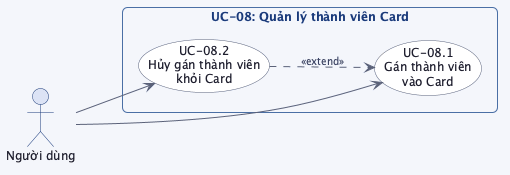
\includegraphics[width=\textwidth]{images/chap3/usecase_uc08.png}
\caption{Biểu đồ Use Case UC-08: Quản lý thành viên Card}
\label{fig:usecase_uc08}
\end{figure}

\vspace{0.3cm}
\noindent\begin{tabular}{|p{3.5cm}|p{10.5cm}|}
\hline
\textbf{Thành phần} & \textbf{Nội dung} \\
\hline
Mã Use Case & UC-08.1 \\
\hline
Tên Use Case & Gán thành viên vào Card \\
\hline
Tác nhân chính & Người dùng \\
\hline
Mô tả tóm tắt & Người dùng gán một thành viên Board làm người phụ trách cho Card. \\
\hline
Điều kiện & Người dùng đã đăng nhập và là thành viên của Board; Card đang mở. \\
\hline
Luồng chính & 1. Người dùng chọn chức năng gán thành viên trong modal Card.\newline 2. Hệ thống hiển thị danh sách thành viên Board có thể gán.\newline 3. Người dùng chọn thành viên cần gán.\newline 4. Hệ thống gọi API POST /api/v1/card-members với userId và cardId.\newline 5. Backend kiểm tra thành viên chưa được gán vào Card này.\newline 6. Backend tạo bản ghi CardMember.\newline 7. Hệ thống hiển thị avatar thành viên trực tiếp trên Card. \\
\hline
Luồng thay thế & Thành viên đã được gán vào Card: Hệ thống hiển thị thông báo trùng lặp.\newline Thành viên không thuộc Board: Hệ thống không cho phép gán.\newline Lỗi không xác định: Hệ thống trả về lỗi HTTP 500. \\
\hline
\end{tabular}

\vspace{0.5cm}
\noindent\begin{tabular}{|p{3.5cm}|p{10.5cm}|}
\hline
\textbf{Thành phần} & \textbf{Nội dung} \\
\hline
Mã Use Case & UC-08.2 \\
\hline
Tên Use Case & Hủy gán thành viên khỏi Card \\
\hline
Tác nhân chính & Người dùng \\
\hline
Mô tả tóm tắt & Người dùng hủy gán thành viên khỏi Card, loại bỏ trách nhiệm phụ trách. \\
\hline
Điều kiện & Người dùng đã đăng nhập và là thành viên của Board; thành viên đã được gán vào Card. \\
\hline
Luồng chính & 1. Người dùng mở modal Card và truy cập danh sách thành viên đã gán.\newline 2. Người dùng chọn thành viên cần hủy gán.\newline 3. Hệ thống gọi API DELETE /api/v1/card-members/:id.\newline 4. Backend xóa bản ghi CardMember.\newline 5. Hệ thống cập nhật danh sách thành viên và xóa avatar khỏi Card. \\
\hline
Luồng thay thế & Bản ghi CardMember không tồn tại: Hệ thống trả về lỗi HTTP 404. \\
\hline
\end{tabular}

\vspace{0.5cm}

\subsubsection{Phân tích luồng nghiệp vụ}

Biểu đồ hoạt động (Activity Diagram) được sử dụng để mô tả trình tự và luồng xử lý của từng chức năng trong hệ thống. Khác với biểu đồ Use Case chỉ trả lời ``Hệ thống làm gì?'', biểu đồ hoạt động trả lời ``Chức năng đó diễn ra như thế nào?'', thể hiện chi tiết các bước xử lý, nhánh điều kiện và luồng thay thế khi xảy ra lỗi.

Phần này trình bày 36 biểu đồ hoạt động, mỗi biểu đồ tương ứng với một use case thành phần (UC-01.1 đến UC-08.2), mô tả chi tiết luồng nghiệp vụ của từng chức năng trong hệ thống Nello.

% ── UC-01 ──────────────────────────────────────────────────────────────────

\paragraph{UC-01: Quản lý xác thực} \mbox{}\\

Nhóm chức năng xác thực bao gồm năm luồng nghiệp vụ: đăng ký tài khoản, xác nhận OTP, gửi lại OTP, đăng nhập và làm mới token. Tất cả các luồng này đều ủy quyền xử lý xác thực cho dịch vụ Amazon Cognito.

\medskip\noindent\textbf{UC-01.1: Đăng ký tài khoản}\medskip

Người dùng nhập thông tin đăng ký; hệ thống xác thực dữ liệu đầu vào, sau đó ủy quyền cho Amazon Cognito tạo tài khoản tạm thời và gửi mã OTP qua email để tiến hành xác nhận.

\begin{figure}[H]
\centering
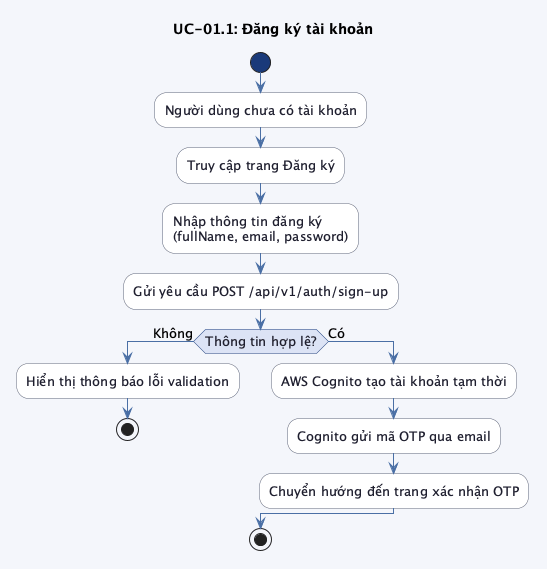
\includegraphics[width=\textwidth, height=0.85\textheight, keepaspectratio]{images/chap3/activity_uc01_1.png}
\caption{Biểu đồ hoạt động UC-01.1: Đăng ký tài khoản}
\label{fig:activity_uc01_1}
\end{figure}

\medskip\noindent\textbf{UC-01.2: Xác nhận tài khoản bằng OTP}\medskip

Người dùng nhập mã OTP nhận được qua email; hệ thống gửi yêu cầu xác nhận đến Cognito, kích hoạt tài khoản nếu mã hợp lệ và chuyển hướng đến trang đăng nhập.

\begin{figure}[H]
\centering
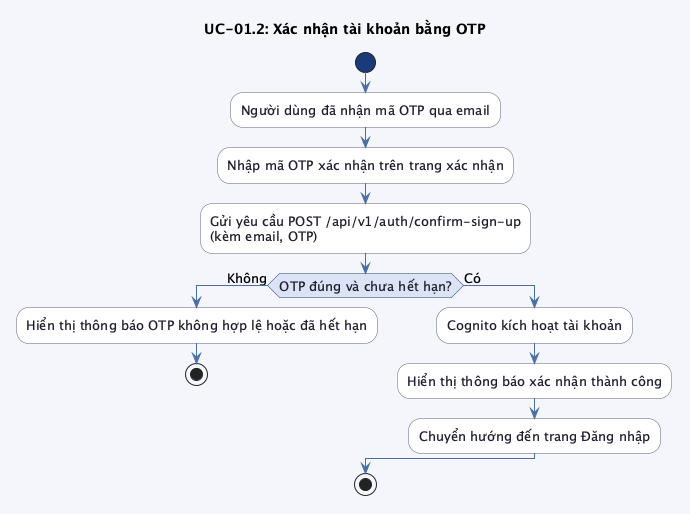
\includegraphics[width=\textwidth, height=0.85\textheight, keepaspectratio]{images/chap3/activity_uc01_2.png}
\caption{Biểu đồ hoạt động UC-01.2: Xác nhận tài khoản bằng OTP}
\label{fig:activity_uc01_2}
\end{figure}

\medskip\noindent\textbf{UC-01.3: Gửi lại mã OTP}\medskip

Khi mã OTP hết hạn hoặc không nhận được, người dùng yêu cầu gửi lại; hệ thống gọi Cognito để phát hành mã OTP mới và gửi về email đã đăng ký.

\begin{figure}[H]
\centering
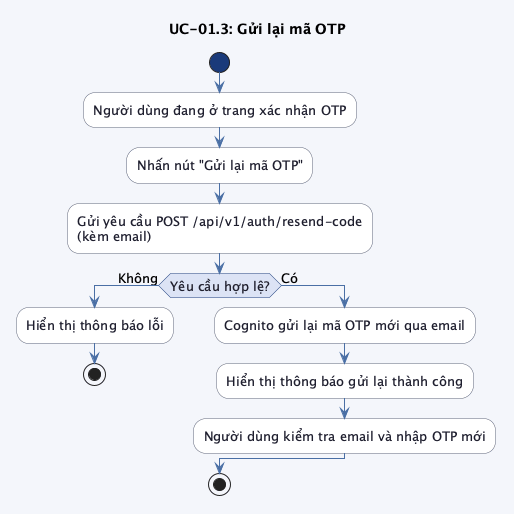
\includegraphics[width=\textwidth, height=0.85\textheight, keepaspectratio]{images/chap3/activity_uc01_3.png}
\caption{Biểu đồ hoạt động UC-01.3: Gửi lại mã OTP}
\label{fig:activity_uc01_3}
\end{figure}

\medskip\noindent\textbf{UC-01.4: Đăng nhập}\medskip

Người dùng nhập thông tin đăng nhập; Cognito xác thực và cấp cặp JWT (access token, refresh token) được lưu vào HttpOnly Cookie, sau đó chuyển hướng đến Dashboard.

\begin{figure}[H]
\centering
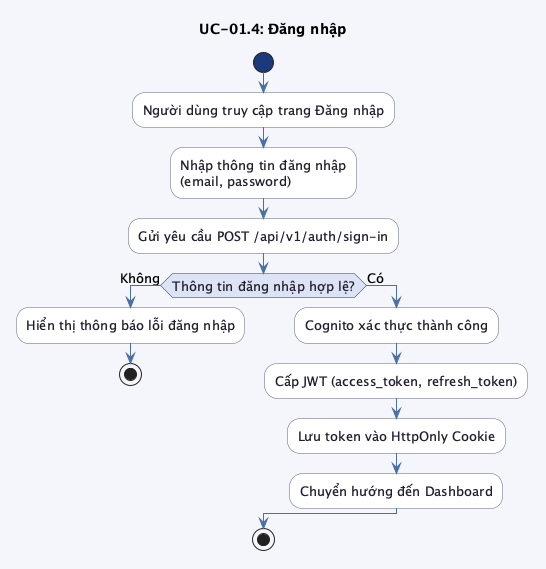
\includegraphics[width=\textwidth, height=0.85\textheight, keepaspectratio]{images/chap3/activity_uc01_4.png}
\caption{Biểu đồ hoạt động UC-01.4: Đăng nhập}
\label{fig:activity_uc01_4}
\end{figure}

\medskip\noindent\textbf{UC-01.5: Làm mới access token}\medskip

Khi access token hết hạn, hệ thống tự động gửi refresh token đến Cognito để lấy access token mới; nếu refresh token không còn hợp lệ, phiên làm việc bị hủy và người dùng được chuyển về trang đăng nhập.

\begin{figure}[H]
\centering
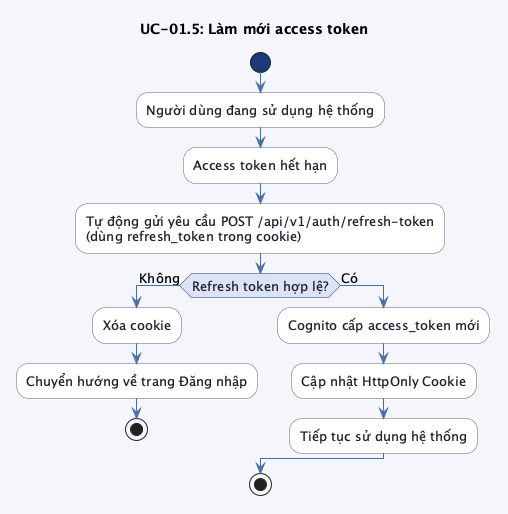
\includegraphics[width=\textwidth, height=0.85\textheight, keepaspectratio]{images/chap3/activity_uc01_5.png}
\caption{Biểu đồ hoạt động UC-01.5: Làm mới access token}
\label{fig:activity_uc01_5}
\end{figure}

% ── UC-02 ──────────────────────────────────────────────────────────────────

\paragraph{UC-02: Quản lý người dùng} \mbox{}\\

Nhóm chức năng quản lý người dùng gồm hai luồng: xem và chỉnh sửa thông tin cá nhân. Cả hai luồng đều yêu cầu token hợp lệ để xác thực danh tính người dùng.

\medskip\noindent\textbf{UC-02.1: Xem thông tin cá nhân}\medskip

Hệ thống xác thực token, gọi API lấy thông tin hồ sơ và hiển thị đầy đủ thông tin cá nhân của người dùng đang đăng nhập.

\begin{figure}[H]
\centering
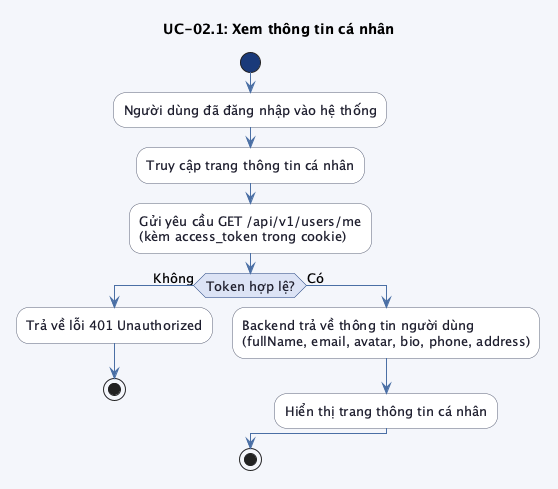
\includegraphics[width=\textwidth, height=0.85\textheight, keepaspectratio]{images/chap3/activity_uc02_1.png}
\caption{Biểu đồ hoạt động UC-02.1: Xem thông tin cá nhân}
\label{fig:activity_uc02_1}
\end{figure}

\medskip\noindent\textbf{UC-02.2: Chỉnh sửa thông tin cá nhân}\medskip

Người dùng tải thông tin hiện tại, chỉnh sửa trên form và gửi yêu cầu cập nhật; hệ thống kiểm tra tính hợp lệ, lưu thay đổi và thông báo kết quả.

\begin{figure}[H]
\centering
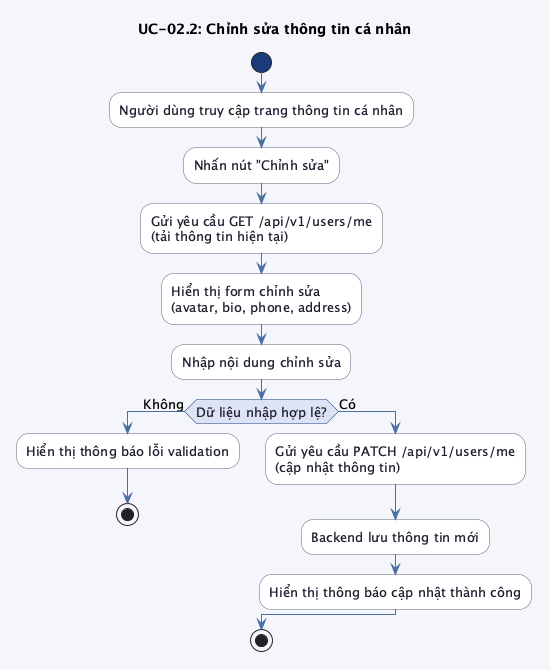
\includegraphics[width=\textwidth, height=0.85\textheight, keepaspectratio]{images/chap3/activity_uc02_2.png}
\caption{Biểu đồ hoạt động UC-02.2: Chỉnh sửa thông tin cá nhân}
\label{fig:activity_uc02_2}
\end{figure}

% ── UC-03 ──────────────────────────────────────────────────────────────────

\paragraph{UC-03: Quản lý Workspace} \mbox{}\\

Nhóm chức năng quản lý Workspace gồm năm luồng: tạo, xem danh sách, xem chi tiết, mời thành viên và xem danh sách thành viên. Người tạo Workspace được tự động gán vai trò quản trị viên.

\medskip\noindent\textbf{UC-03.1: Tạo Workspace}\medskip

Người dùng nhập tên, chọn danh mục và mô tả; hệ thống tạo Workspace và gán người tạo vai trò ADMIN, sau đó chuyển hướng đến trang chi tiết vừa tạo.

\begin{figure}[H]
\centering
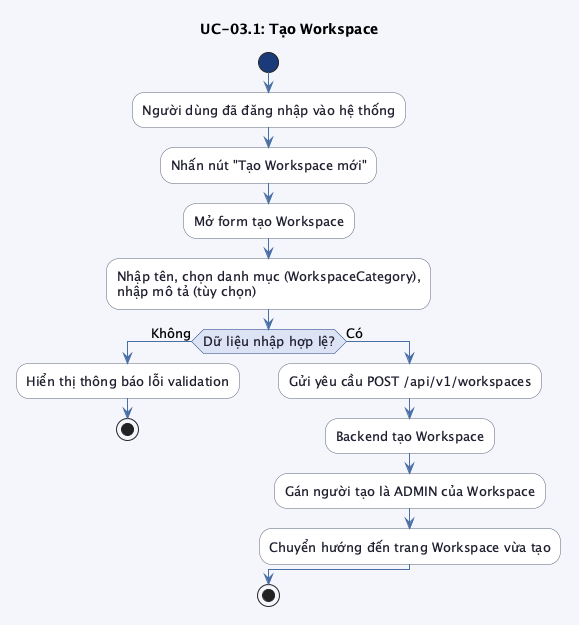
\includegraphics[width=\textwidth, height=0.85\textheight, keepaspectratio]{images/chap3/activity_uc03_1.png}
\caption{Biểu đồ hoạt động UC-03.1: Tạo Workspace}
\label{fig:activity_uc03_1}
\end{figure}

\medskip\noindent\textbf{UC-03.2: Xem danh sách Workspace}\medskip

Hệ thống tải toàn bộ Workspace mà người dùng sở hữu hoặc là thành viên và hiển thị trên trang Dashboard.

\begin{figure}[H]
\centering
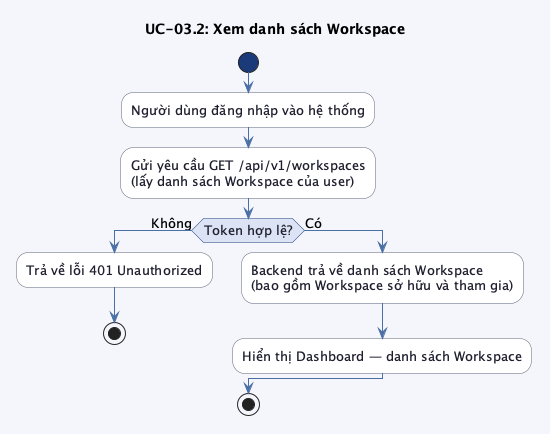
\includegraphics[width=\textwidth, height=0.85\textheight, keepaspectratio]{images/chap3/activity_uc03_2.png}
\caption{Biểu đồ hoạt động UC-03.2: Xem danh sách Workspace}
\label{fig:activity_uc03_2}
\end{figure}

\medskip\noindent\textbf{UC-03.3: Xem chi tiết Workspace}\medskip

Hệ thống kiểm tra quyền truy cập và trả về thông tin Workspace gồm tên, danh mục, mô tả, danh sách Board và thành viên.

\begin{figure}[H]
\centering
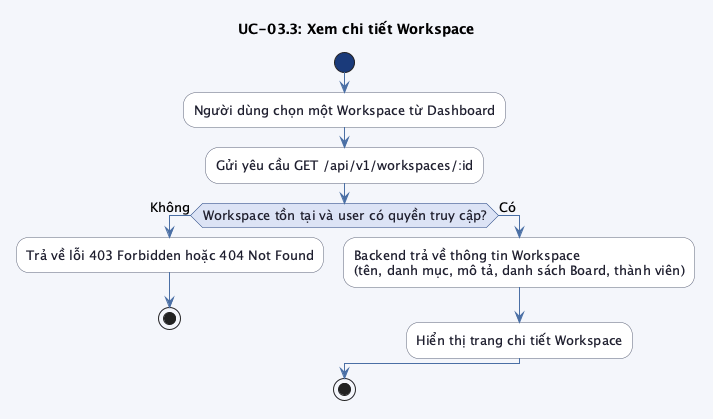
\includegraphics[width=\textwidth, height=0.85\textheight, keepaspectratio]{images/chap3/activity_uc03_3.png}
\caption{Biểu đồ hoạt động UC-03.3: Xem chi tiết Workspace}
\label{fig:activity_uc03_3}
\end{figure}

\medskip\noindent\textbf{UC-03.4: Mời thành viên vào Workspace}\medskip

Quản trị viên nhập email người dùng cần mời; hệ thống xác minh email tồn tại trong hệ thống, thêm thành viên với vai trò MEMBER và thông báo kết quả.

\begin{figure}[H]
\centering
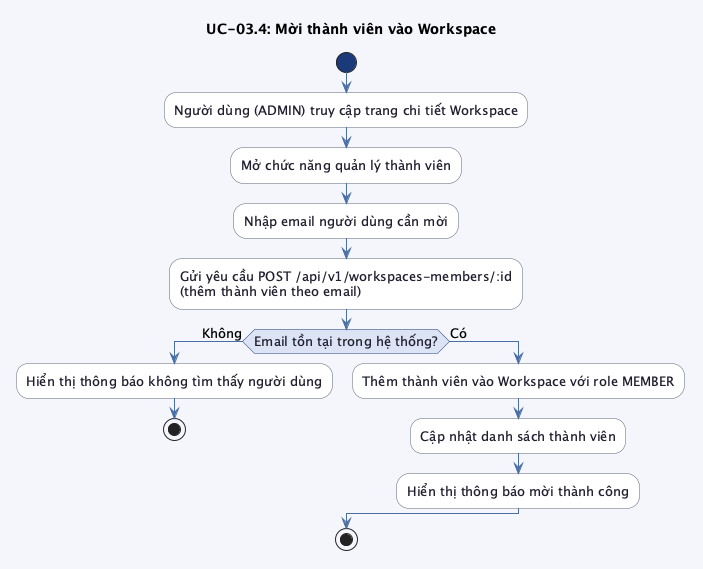
\includegraphics[width=\textwidth, height=0.85\textheight, keepaspectratio]{images/chap3/activity_uc03_4.png}
\caption{Biểu đồ hoạt động UC-03.4: Mời thành viên vào Workspace}
\label{fig:activity_uc03_4}
\end{figure}

\medskip\noindent\textbf{UC-03.5: Xem danh sách thành viên Workspace}\medskip

Hệ thống xác thực quyền truy cập và trả về danh sách thành viên Workspace kèm vai trò và thông tin cá nhân tương ứng.

\begin{figure}[H]
\centering
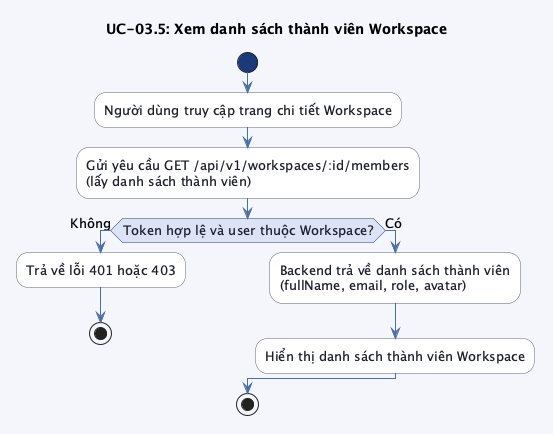
\includegraphics[width=\textwidth, height=0.85\textheight, keepaspectratio]{images/chap3/activity_uc03_5.png}
\caption{Biểu đồ hoạt động UC-03.5: Xem danh sách thành viên Workspace}
\label{fig:activity_uc03_5}
\end{figure}

% ── UC-04 ──────────────────────────────────────────────────────────────────

\paragraph{UC-04: Quản lý Board} \mbox{}\\

Nhóm chức năng quản lý Board gồm năm luồng: tạo, xem chi tiết, cập nhật tên, xóa và thêm thành viên. Các thao tác thay đổi cấu trúc Board yêu cầu người dùng có vai trò quản trị viên.

\medskip\noindent\textbf{UC-04.1: Tạo Board}\medskip

Người dùng nhập tên và chọn ảnh nền từ danh sách có sẵn; hệ thống khởi tạo Board trong Workspace và chuyển hướng đến giao diện Kanban.

\begin{figure}[H]
\centering
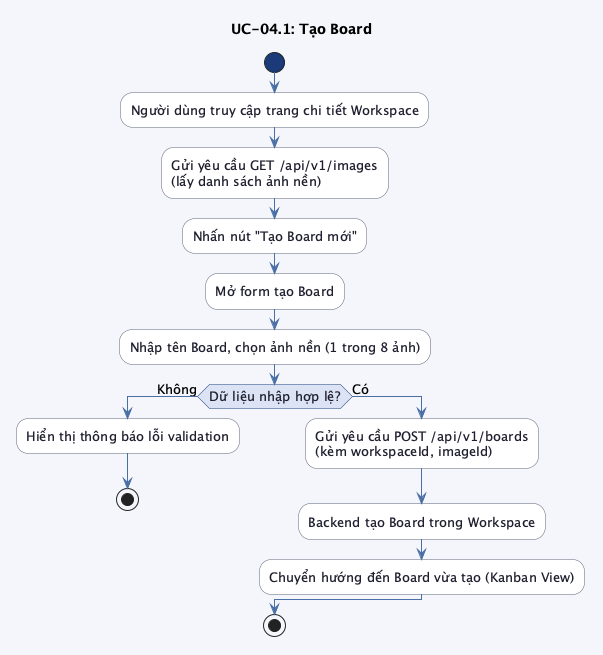
\includegraphics[width=\textwidth, height=0.85\textheight, keepaspectratio]{images/chap3/activity_uc04_1.png}
\caption{Biểu đồ hoạt động UC-04.1: Tạo Board}
\label{fig:activity_uc04_1}
\end{figure}

\medskip\noindent\textbf{UC-04.2: Xem chi tiết Board}\medskip

Hệ thống kiểm tra quyền truy cập, tải toàn bộ dữ liệu Board bao gồm các List và Card, rồi hiển thị theo dạng Kanban.

\begin{figure}[H]
\centering
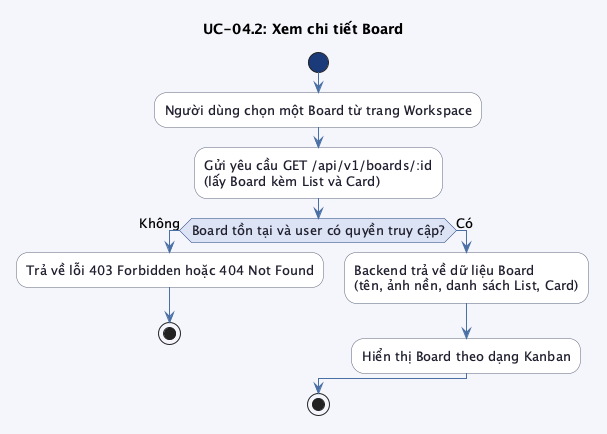
\includegraphics[width=\textwidth, height=0.85\textheight, keepaspectratio]{images/chap3/activity_uc04_2.png}
\caption{Biểu đồ hoạt động UC-04.2: Xem chi tiết Board}
\label{fig:activity_uc04_2}
\end{figure}

\medskip\noindent\textbf{UC-04.3: Cập nhật tên Board}\medskip

Người dùng chỉnh sửa tiêu đề Board trực tiếp trên giao diện; hệ thống xác thực và lưu tên mới, thông báo cập nhật thành công.

\begin{figure}[H]
\centering
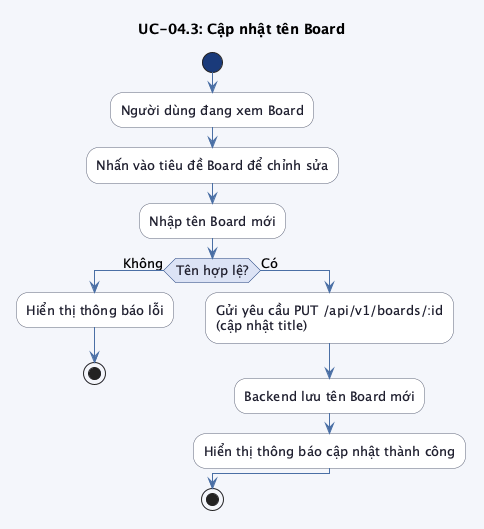
\includegraphics[width=\textwidth, height=0.85\textheight, keepaspectratio]{images/chap3/activity_uc04_3.png}
\caption{Biểu đồ hoạt động UC-04.3: Cập nhật tên Board}
\label{fig:activity_uc04_3}
\end{figure}

\medskip\noindent\textbf{UC-04.4: Xóa Board}\medskip

Sau khi xác nhận xóa, hệ thống xóa Board cùng toàn bộ dữ liệu liên quan (List, Card, Checklist) theo cơ chế cascade và chuyển hướng về trang Workspace.

\begin{figure}[H]
\centering
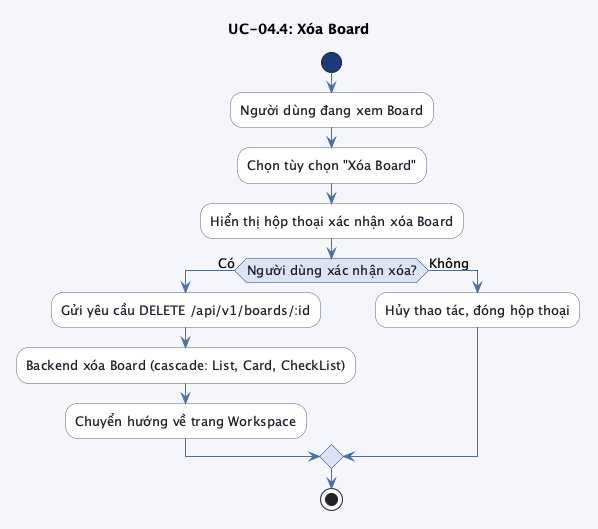
\includegraphics[width=\textwidth, height=0.85\textheight, keepaspectratio]{images/chap3/activity_uc04_4.png}
\caption{Biểu đồ hoạt động UC-04.4: Xóa Board}
\label{fig:activity_uc04_4}
\end{figure}

\medskip\noindent\textbf{UC-04.5: Thêm thành viên vào Board}\medskip

Quản trị viên chọn thành viên từ danh sách Workspace và gán vai trò; hệ thống thêm thành viên vào Board với quyền hạn tương ứng.

\begin{figure}[H]
\centering
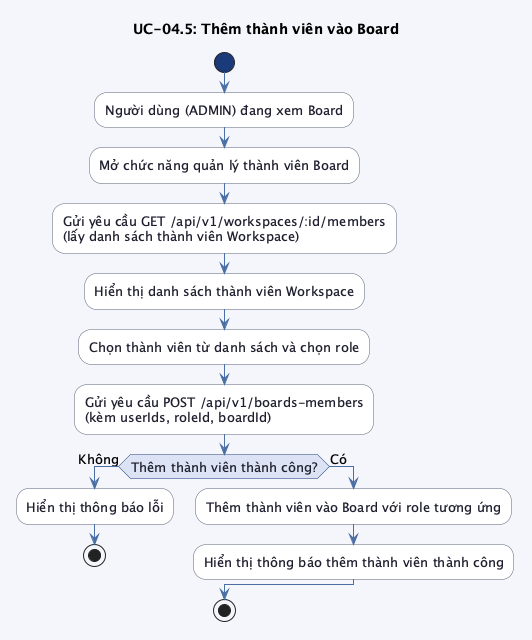
\includegraphics[width=\textwidth, height=0.85\textheight, keepaspectratio]{images/chap3/activity_uc04_5.png}
\caption{Biểu đồ hoạt động UC-04.5: Thêm thành viên vào Board}
\label{fig:activity_uc04_5}
\end{figure}

% ── UC-05 ──────────────────────────────────────────────────────────────────

\paragraph{UC-05: Quản lý List} \mbox{}\\

Nhóm chức năng quản lý List gồm bốn luồng: tạo, đổi tên, xóa và sắp xếp thứ tự. Tính năng sắp xếp áp dụng optimistic update để đảm bảo trải nghiệm tương tác tức thì.

\medskip\noindent\textbf{UC-05.1: Tạo List}\medskip

Người dùng nhập tên List mới; hệ thống lưu List với vị trí cuối cùng trong Board và hiển thị cột mới trên giao diện Kanban.

\begin{figure}[H]
\centering
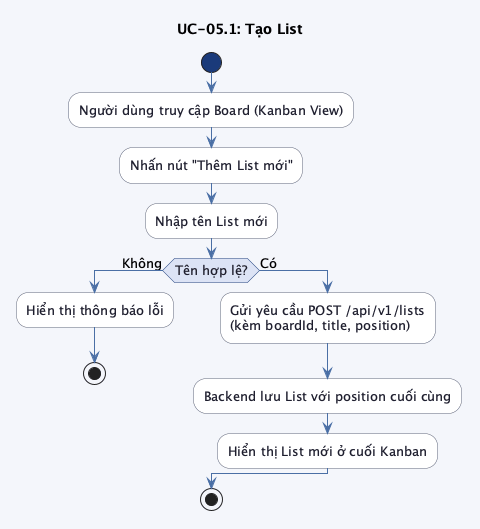
\includegraphics[width=\textwidth, height=0.85\textheight, keepaspectratio]{images/chap3/activity_uc05_1.png}
\caption{Biểu đồ hoạt động UC-05.1: Tạo List}
\label{fig:activity_uc05_1}
\end{figure}

\medskip\noindent\textbf{UC-05.2: Đổi tên List}\medskip

Người dùng chỉnh sửa tiêu đề List trực tiếp; hệ thống xác thực và cập nhật tên mới lên giao diện và cơ sở dữ liệu.

\begin{figure}[H]
\centering
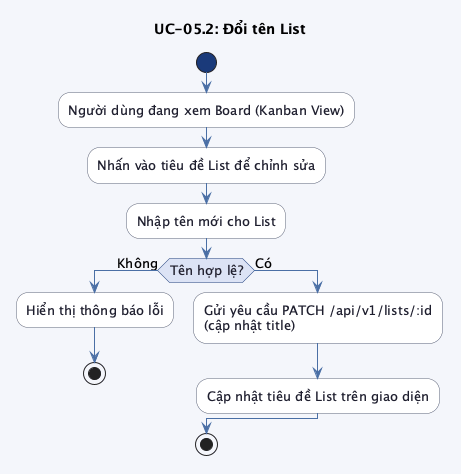
\includegraphics[width=\textwidth, height=0.85\textheight, keepaspectratio]{images/chap3/activity_uc05_2.png}
\caption{Biểu đồ hoạt động UC-05.2: Đổi tên List}
\label{fig:activity_uc05_2}
\end{figure}

\medskip\noindent\textbf{UC-05.3: Xóa List}\medskip

Sau khi xác nhận, hệ thống xóa List và toàn bộ dữ liệu liên quan (Card, Checklist, ChecklistItem) theo cơ chế cascade, đồng thời xóa cột tương ứng khỏi giao diện Kanban.

\begin{figure}[H]
\centering
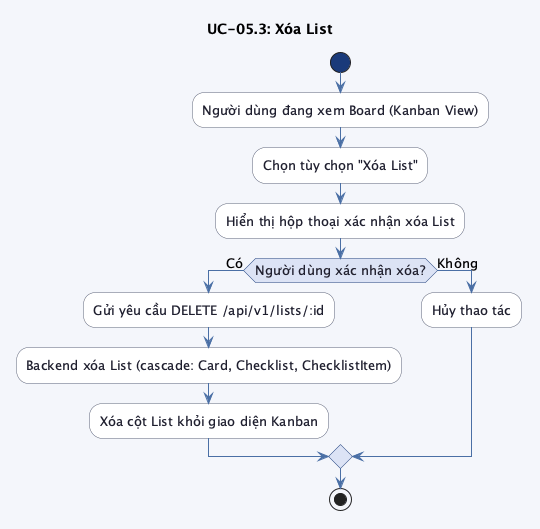
\includegraphics[width=\textwidth, height=0.85\textheight, keepaspectratio]{images/chap3/activity_uc05_3.png}
\caption{Biểu đồ hoạt động UC-05.3: Xóa List}
\label{fig:activity_uc05_3}
\end{figure}

\medskip\noindent\textbf{UC-05.4: Sắp xếp thứ tự List}\medskip

Người dùng kéo thả List sang vị trí mới; giao diện cập nhật tức thì (optimistic update) và đồng bộ với máy chủ; nếu thất bại, giao diện tự động khôi phục về thứ tự cũ.

\begin{figure}[H]
\centering
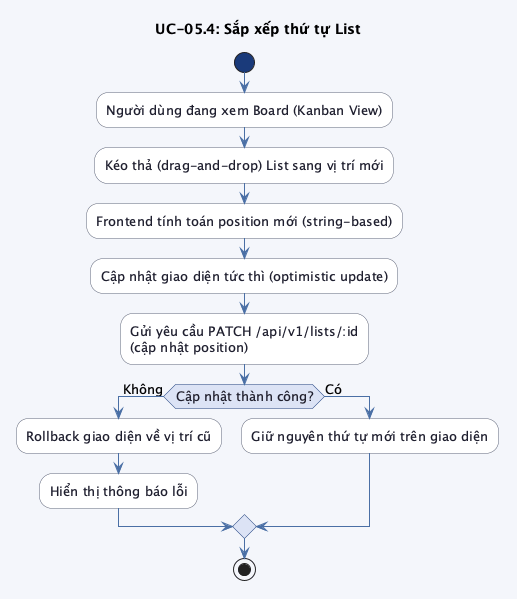
\includegraphics[width=\textwidth, height=0.85\textheight, keepaspectratio]{images/chap3/activity_uc05_4.png}
\caption{Biểu đồ hoạt động UC-05.4: Sắp xếp thứ tự List}
\label{fig:activity_uc05_4}
\end{figure}

% ── UC-06 ──────────────────────────────────────────────────────────────────

\paragraph{UC-06: Quản lý Card} \mbox{}\\

Nhóm chức năng quản lý Card gồm sáu luồng: tạo, xem chi tiết, cập nhật, đánh dấu hoàn thành, di chuyển giữa các List và xóa. Card là thực thể trung tâm của hệ thống, liên kết với Checklist và thành viên phụ trách.

\medskip\noindent\textbf{UC-06.1: Tạo Card}\medskip

Người dùng nhập tiêu đề Card trong một List; hệ thống lưu Card với vị trí cuối cùng trong List và hiển thị Card mới trên cột Kanban.

\begin{figure}[H]
\centering
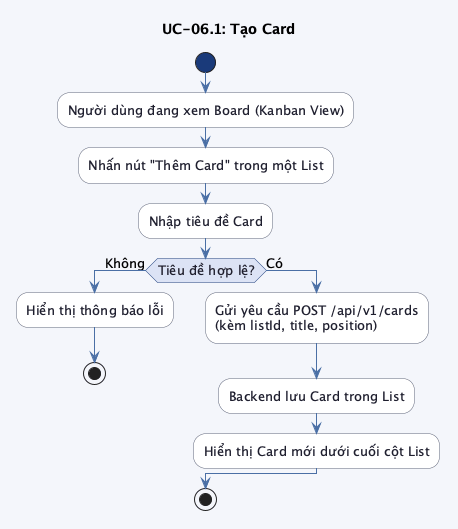
\includegraphics[width=\textwidth, height=0.85\textheight, keepaspectratio]{images/chap3/activity_uc06_1.png}
\caption{Biểu đồ hoạt động UC-06.1: Tạo Card}
\label{fig:activity_uc06_1}
\end{figure}

\medskip\noindent\textbf{UC-06.2: Xem chi tiết Card}\medskip

Hệ thống kiểm tra quyền truy cập và trả về đầy đủ thông tin Card gồm tiêu đề, mô tả, ngày hạn, Checklist và danh sách thành viên phụ trách, hiển thị trong Card Detail Modal.

\begin{figure}[H]
\centering
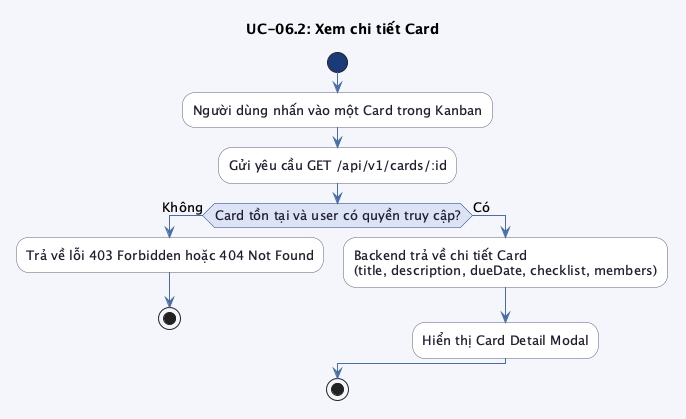
\includegraphics[width=\textwidth, height=0.85\textheight, keepaspectratio]{images/chap3/activity_uc06_2.png}
\caption{Biểu đồ hoạt động UC-06.2: Xem chi tiết Card}
\label{fig:activity_uc06_2}
\end{figure}

\medskip\noindent\textbf{UC-06.3: Cập nhật Card}\medskip

Người dùng chỉnh sửa các trường thông tin của Card (tiêu đề, mô tả, ngày bắt đầu, ngày đến hạn); hệ thống xác thực dữ liệu và lưu thay đổi.

\begin{figure}[H]
\centering
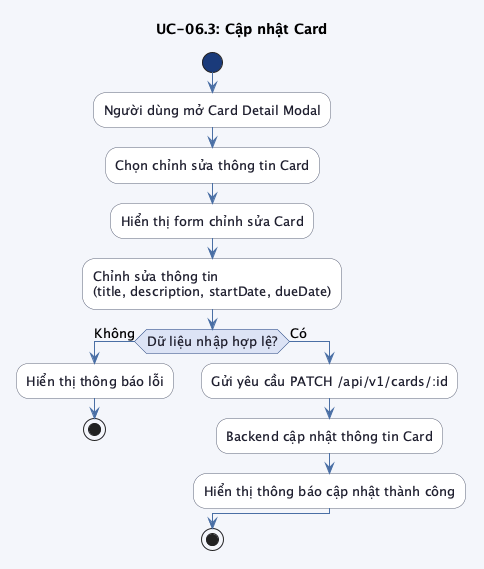
\includegraphics[width=\textwidth, height=0.85\textheight, keepaspectratio]{images/chap3/activity_uc06_3.png}
\caption{Biểu đồ hoạt động UC-06.3: Cập nhật Card}
\label{fig:activity_uc06_3}
\end{figure}

\medskip\noindent\textbf{UC-06.4: Đánh dấu Card hoàn thành}\medskip

Người dùng nhấn nút đánh dấu hoàn thành; hệ thống cập nhật trạng thái \texttt{isCompleted = true} và phản ánh thay đổi trên giao diện Card.

\begin{figure}[H]
\centering
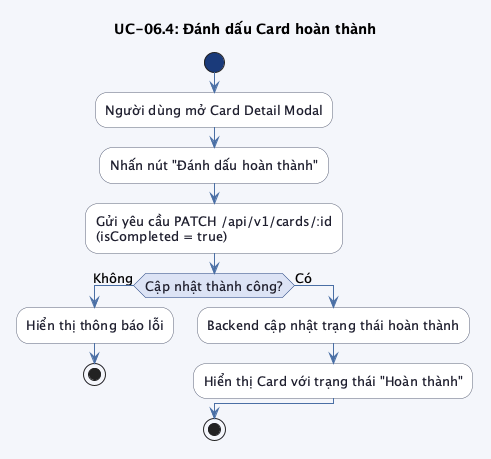
\includegraphics[width=\textwidth, height=0.85\textheight, keepaspectratio]{images/chap3/activity_uc06_4.png}
\caption{Biểu đồ hoạt động UC-06.4: Đánh dấu Card hoàn thành}
\label{fig:activity_uc06_4}
\end{figure}

\medskip\noindent\textbf{UC-06.5: Di chuyển Card giữa các List}\medskip

Người dùng kéo thả Card sang List đích; giao diện cập nhật tức thì (optimistic update) và đồng bộ vị trí mới với máy chủ; nếu thất bại, Card được khôi phục về vị trí ban đầu.

\begin{figure}[H]
\centering
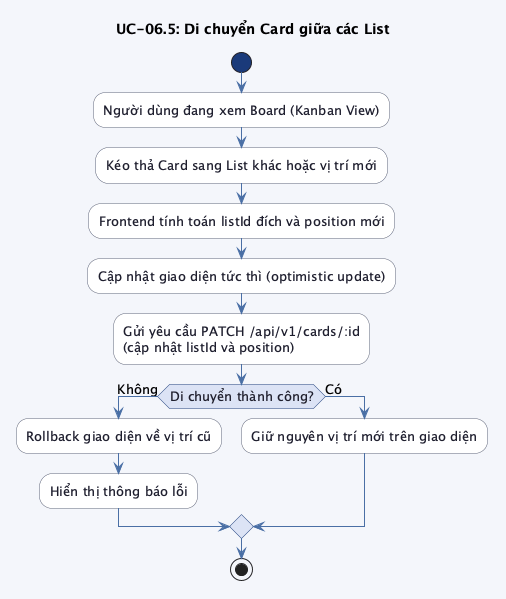
\includegraphics[width=\textwidth, height=0.85\textheight, keepaspectratio]{images/chap3/activity_uc06_5.png}
\caption{Biểu đồ hoạt động UC-06.5: Di chuyển Card giữa các List}
\label{fig:activity_uc06_5}
\end{figure}

\medskip\noindent\textbf{UC-06.6: Xóa Card}\medskip

Sau khi xác nhận, hệ thống xóa Card và toàn bộ dữ liệu liên quan (Checklist, ChecklistItem, CardMember) theo cơ chế cascade.

\begin{figure}[H]
\centering
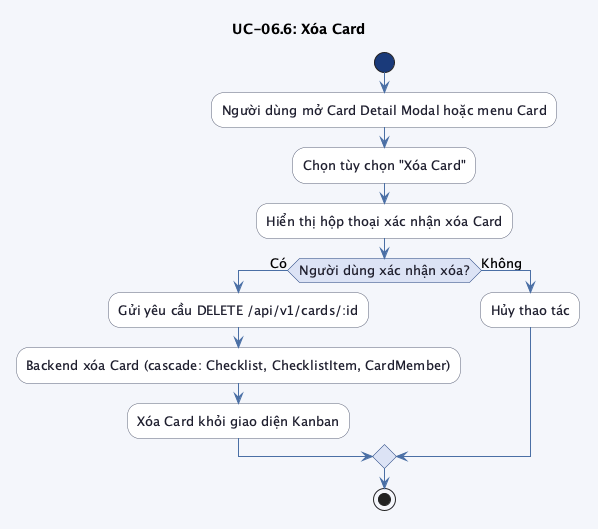
\includegraphics[width=\textwidth, height=0.85\textheight, keepaspectratio]{images/chap3/activity_uc06_6.png}
\caption{Biểu đồ hoạt động UC-06.6: Xóa Card}
\label{fig:activity_uc06_6}
\end{figure}

% ── UC-07 ──────────────────────────────────────────────────────────────────

\paragraph{UC-07: Quản lý Checklist} \mbox{}\\

Nhóm chức năng quản lý Checklist gồm bảy luồng: tạo, cập nhật và xóa Checklist; tạo, cập nhật, đánh dấu hoàn thành và xóa Checklist Item. Thanh tiến độ (progress bar) được cập nhật tức thì sau mỗi thay đổi trạng thái Item.

\medskip\noindent\textbf{UC-07.1: Tạo Checklist}\medskip

Người dùng nhập tên Checklist trong Card Detail Modal; hệ thống lưu Checklist và hiển thị ngay trong giao diện Card.

\begin{figure}[H]
\centering
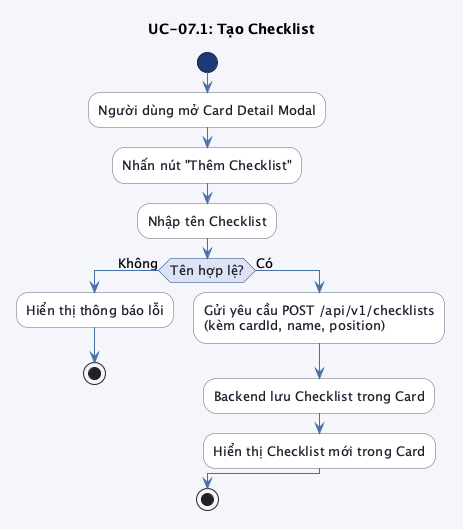
\includegraphics[width=\textwidth, height=0.85\textheight, keepaspectratio]{images/chap3/activity_uc07_1.png}
\caption{Biểu đồ hoạt động UC-07.1: Tạo Checklist}
\label{fig:activity_uc07_1}
\end{figure}

\medskip\noindent\textbf{UC-07.2: Cập nhật Checklist}\medskip

Người dùng chỉnh sửa tên Checklist; hệ thống lưu thông tin mới và cập nhật giao diện.

\begin{figure}[H]
\centering
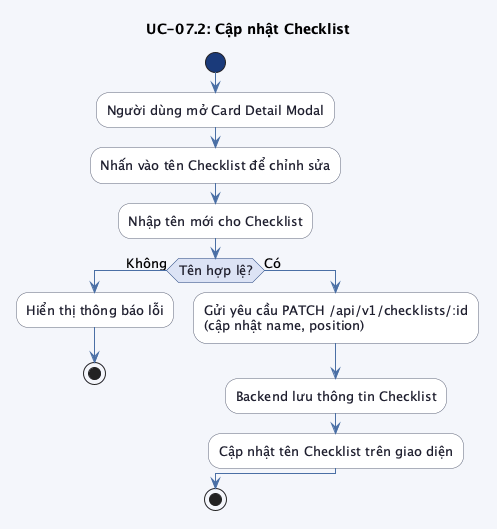
\includegraphics[width=\textwidth, height=0.85\textheight, keepaspectratio]{images/chap3/activity_uc07_2.png}
\caption{Biểu đồ hoạt động UC-07.2: Cập nhật Checklist}
\label{fig:activity_uc07_2}
\end{figure}

\medskip\noindent\textbf{UC-07.3: Xóa Checklist}\medskip

Sau khi xác nhận, hệ thống xóa Checklist và toàn bộ ChecklistItem bên trong theo cơ chế cascade.

\begin{figure}[H]
\centering
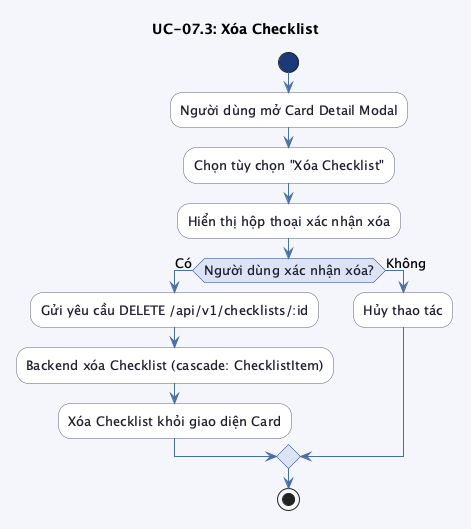
\includegraphics[width=\textwidth, height=0.85\textheight, keepaspectratio]{images/chap3/activity_uc07_3.png}
\caption{Biểu đồ hoạt động UC-07.3: Xóa Checklist}
\label{fig:activity_uc07_3}
\end{figure}

\medskip\noindent\textbf{UC-07.4: Tạo Checklist Item}\medskip

Người dùng nhập tên Item trong một Checklist; hệ thống lưu Item với vị trí cuối cùng và hiển thị ngay trong danh sách.

\begin{figure}[H]
\centering
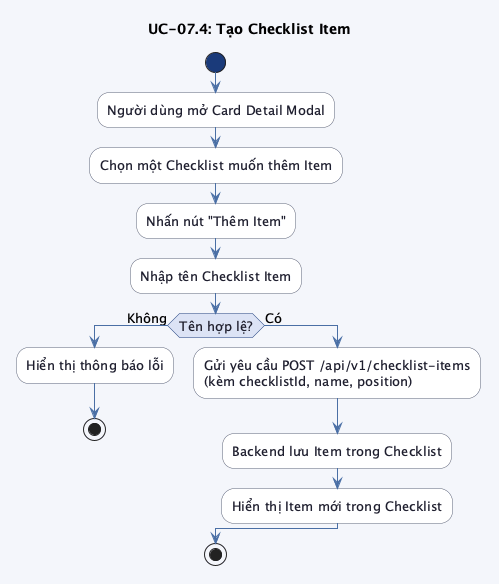
\includegraphics[width=\textwidth, height=0.85\textheight, keepaspectratio]{images/chap3/activity_uc07_4.png}
\caption{Biểu đồ hoạt động UC-07.4: Tạo Checklist Item}
\label{fig:activity_uc07_4}
\end{figure}

\medskip\noindent\textbf{UC-07.5: Cập nhật Checklist Item}\medskip

Người dùng chỉnh sửa tên hoặc ngày đến hạn của Item; hệ thống xác thực và lưu thay đổi lên cơ sở dữ liệu.

\begin{figure}[H]
\centering
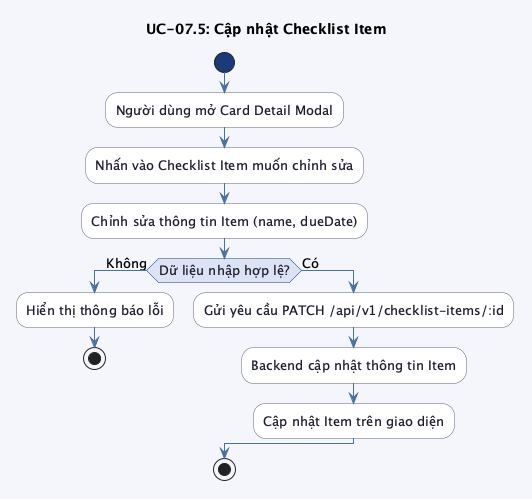
\includegraphics[width=\textwidth, height=0.85\textheight, keepaspectratio]{images/chap3/activity_uc07_5.png}
\caption{Biểu đồ hoạt động UC-07.5: Cập nhật Checklist Item}
\label{fig:activity_uc07_5}
\end{figure}

\medskip\noindent\textbf{UC-07.6: Đánh dấu Checklist Item hoàn thành}\medskip

Người dùng tick checkbox của Item; hệ thống cập nhật trạng thái \texttt{isCompleted} và làm mới thanh tiến độ của Checklist tương ứng.

\begin{figure}[H]
\centering
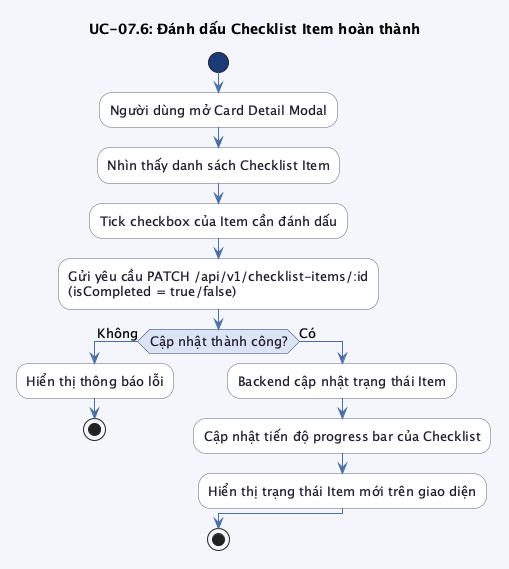
\includegraphics[width=\textwidth, height=0.85\textheight, keepaspectratio]{images/chap3/activity_uc07_6.png}
\caption{Biểu đồ hoạt động UC-07.6: Đánh dấu Checklist Item hoàn thành}
\label{fig:activity_uc07_6}
\end{figure}

\medskip\noindent\textbf{UC-07.7: Xóa Checklist Item}\medskip

Sau khi xác nhận, hệ thống xóa Item và cập nhật thanh tiến độ của Checklist phản ánh số lượng Item còn lại.

\begin{figure}[H]
\centering
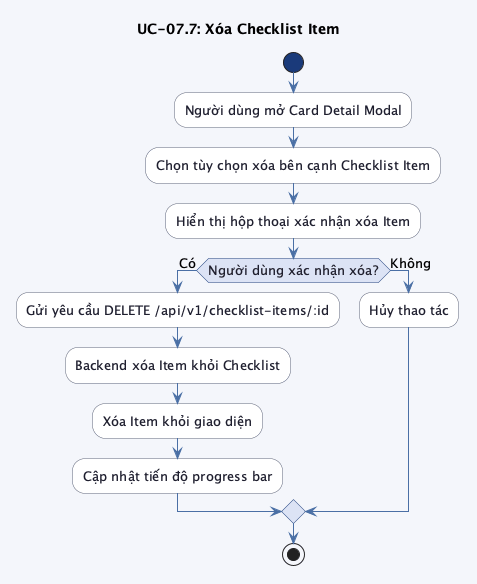
\includegraphics[width=\textwidth, height=0.85\textheight, keepaspectratio]{images/chap3/activity_uc07_7.png}
\caption{Biểu đồ hoạt động UC-07.7: Xóa Checklist Item}
\label{fig:activity_uc07_7}
\end{figure}

% ── UC-08 ──────────────────────────────────────────────────────────────────

\paragraph{UC-08: Quản lý thành viên Card} \mbox{}\\

Nhóm chức năng quản lý thành viên Card gồm hai luồng: gán và hủy gán thành viên phụ trách. Hệ thống chỉ cho phép gán thành viên đã có trong Board, ngăn trùng lặp.

\medskip\noindent\textbf{UC-08.1: Gán thành viên vào Card}\medskip

Hệ thống tải danh sách thành viên Board chưa được gán vào Card; người dùng chọn thành viên và hệ thống thêm vào danh sách phụ trách, cập nhật giao diện Card ngay lập tức.

\begin{figure}[H]
\centering
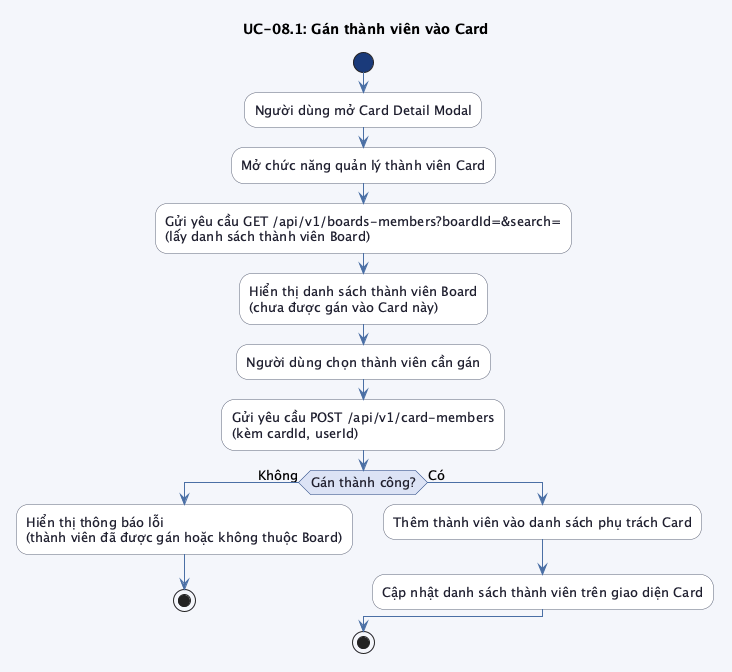
\includegraphics[width=\textwidth, height=0.85\textheight, keepaspectratio]{images/chap3/activity_uc08_1.png}
\caption{Biểu đồ hoạt động UC-08.1: Gán thành viên vào Card}
\label{fig:activity_uc08_1}
\end{figure}

\medskip\noindent\textbf{UC-08.2: Hủy gán thành viên khỏi Card}\medskip

Người dùng chọn thành viên cần gỡ bỏ khỏi Card; hệ thống xóa quan hệ gán và cập nhật danh sách phụ trách trên giao diện.

\begin{figure}[H]
\centering
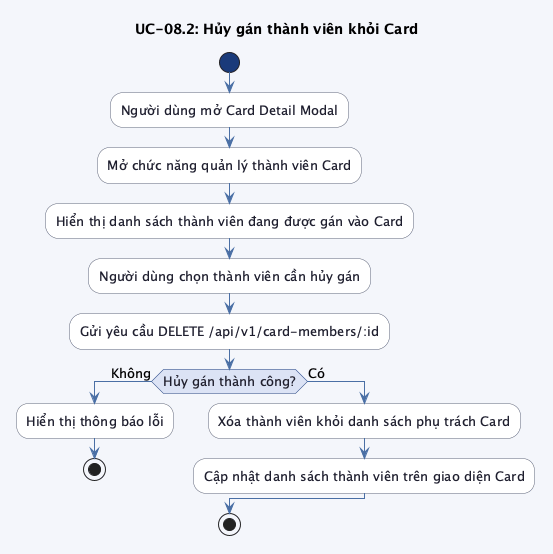
\includegraphics[width=\textwidth, height=0.85\textheight, keepaspectratio]{images/chap3/activity_uc08_2.png}
\caption{Biểu đồ hoạt động UC-08.2: Hủy gán thành viên khỏi Card}
\label{fig:activity_uc08_2}
\end{figure}

\subsubsection{Phân tích dữ liệu}

\paragraph{Các thực thể chính} \mbox{}\\

Hệ thống xoay quanh sáu thực thể nghiệp vụ chính được tổ chức theo cấu trúc phân cấp:

\begin{itemize}
    \item \textbf{User (Người dùng):} Đại diện cho tài khoản người dùng trong hệ thống. Thông tin danh tính và xác thực được quản lý bởi Amazon Cognito; hệ thống nội bộ lưu trữ thông tin bổ sung như họ tên, ảnh đại diện và mã định danh Cognito.
    \item \textbf{Workspace (Không gian làm việc):} Đơn vị tổ chức cấp cao nhất, quản lý tập trung nhiều Board liên quan. Mỗi Workspace có một người sở hữu (owner) và nhiều thành viên.
    \item \textbf{Board (Bảng công việc):} Đại diện cho một dự án cụ thể trong Workspace. Mỗi Board chứa nhiều List và có danh sách thành viên riêng.
    \item \textbf{List (Danh sách):} Cột trạng thái trong Board, thể hiện giai đoạn thực hiện của công việc. Thứ tự các List được quản lý qua trường \texttt{position}.
    \item \textbf{Card (Thẻ công việc):} Đơn vị công việc cơ bản, chứa thông tin chi tiết về nhiệm vụ cần thực hiện. Card thuộc về một List và có thứ tự xác định bằng \texttt{position}.
    \item \textbf{Checklist:} Danh sách kiểm tra trong Card, hỗ trợ theo dõi các công việc con. Mỗi Checklist có nhiều ChecklistItem.
    \item \textbf{ChecklistItem:} Hạng mục cụ thể trong Checklist, có thể được đánh dấu hoàn thành hoặc chưa hoàn thành, và có thể thiết lập thời hạn riêng.
\end{itemize}

\paragraph{Quan hệ giữa các thực thể} \mbox{}\\

\begin{itemize}
    \item Một \textbf{User} có thể sở hữu nhiều \textbf{Workspace} và là thành viên của nhiều \textbf{Workspace} và \textbf{Board} khác.
    \item Một \textbf{Workspace} chứa nhiều \textbf{Board} và có nhiều \textbf{User} làm thành viên (quan hệ nhiều-nhiều qua bảng \texttt{workspace\_member}).
    \item Một \textbf{Board} chứa nhiều \textbf{List} và có nhiều \textbf{User} làm thành viên với các vai trò khác nhau (quan hệ nhiều-nhiều qua bảng \texttt{board\_member}).
    \item Một \textbf{List} chứa nhiều \textbf{Card}; các Card được sắp xếp theo thứ tự \texttt{position}.
    \item Một \textbf{Card} có thể chứa nhiều \textbf{Checklist} và được gán cho nhiều \textbf{User} (quan hệ nhiều-nhiều qua bảng \texttt{card\_member}).
    \item Một \textbf{Checklist} chứa nhiều \textbf{ChecklistItem}.
\end{itemize}

\subsection{Thiết kế hệ thống}

\subsubsection{Thiết kế kiến trúc tổng thể}

Hệ thống Nello áp dụng kiến trúc \textbf{Client-Server phân tách hoàn toàn} (decoupled Frontend/Backend). Frontend và Backend là hai ứng dụng độc lập, giao tiếp với nhau thông qua RESTful API. Toàn bộ logic nghiệp vụ được xử lý tập trung tại Backend; Frontend chịu trách nhiệm trình bày giao diện và tương tác người dùng.

\paragraph{Phân tầng hệ thống} \mbox{}\\

Hệ thống được tổ chức thành ba tầng chính:

\begin{itemize}
    \item \textbf{Frontend (ReactJS):} Ứng dụng chạy trên trình duyệt, bao gồm ba nhóm giao diện chính: xác thực (Auth Pages), quản lý Workspace và Dashboard, và giao diện Kanban (Board/List/Card). Frontend giao tiếp với Backend qua REST API sử dụng JSON, token được lưu trong HttpOnly Cookie.

    \item \textbf{Backend (Spring Boot):} Cung cấp toàn bộ RESTful API tại base path \texttt{/api/v1}. Kiến trúc nội bộ Backend tuân theo mô hình phân lớp gồm ba tầng:
    \begin{itemize}
        \item \textbf{Controller Layer:} Tiếp nhận HTTP request, kiểm tra JWT từ cookie, ủy quyền xử lý cho Service Layer và trả về HTTP response chuẩn hóa.
        \item \textbf{Service Layer:} Chứa toàn bộ logic nghiệp vụ, điều phối giữa Repository và các dịch vụ ngoài (Cognito, S3).
        \item \textbf{Repository Layer:} Truy xuất và lưu trữ dữ liệu thông qua Spring Data JPA, giao tiếp trực tiếp với PostgreSQL qua JDBC.
    \end{itemize}

    \item \textbf{Dịch vụ ngoài (AWS):} Gồm Amazon Cognito (xác thực người dùng và cấp JWT), PostgreSQL trên AWS RDS (cơ sở dữ liệu chính), và Amazon S3 (lưu trữ tệp đa phương tiện).
\end{itemize}

\begin{figure}[H]
\centering
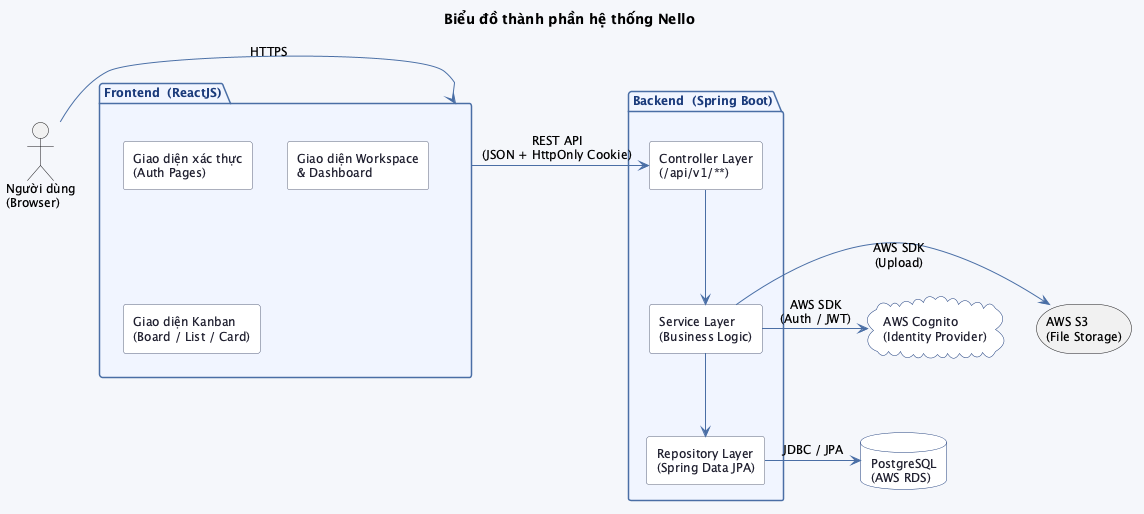
\includegraphics[width=\textwidth, height=0.75\textheight, keepaspectratio]{images/chap3/component_system.png}
\caption{Biểu đồ thành phần hệ thống Nello}
\label{fig:component_system}
\end{figure}

\paragraph{Kiến trúc triển khai} \mbox{}\\

Hệ thống được triển khai trên nền tảng AWS với toàn bộ máy chủ và cơ sở dữ liệu đặt trong một Virtual Private Cloud (VPC) riêng biệt, cách ly hoàn toàn với Internet. Các thành phần triển khai chính gồm:

\begin{itemize}
    \item \textbf{Amazon ALB (Application Load Balancer):} Điểm vào (entry point) duy nhất nhận lưu lượng từ Internet, phân phối request đến EC2 Frontend hoặc EC2 Backend trong mạng private.

    \item \textbf{EC2 (Frontend):} Ứng dụng ReactJS được đóng gói bằng Docker và phục vụ qua Nginx. Chỉ nhận lưu lượng từ ALB, không tiếp xúc trực tiếp với Internet.

    \item \textbf{EC2 (Backend):} Ứng dụng Spring Boot xử lý API. Chỉ nhận request nội bộ từ ALB và giao tiếp với RDS và Cognito.

    \item \textbf{Amazon RDS (PostgreSQL):} Cơ sở dữ liệu quan hệ trong mạng private sâu nhất, chỉ Backend mới được phép truy cập.

    \item \textbf{Amazon CloudFront + S3:} CloudFront đóng vai trò CDN phân phối tài nguyên tĩnh từ S3 đến người dùng với độ trễ thấp.
\end{itemize}

Luồng hoạt động chính gồm ba hướng: (1) Tải giao diện: Client $\to$ ALB $\to$ EC2 Frontend; (2) Tài nguyên tĩnh: Client $\to$ CloudFront $\to$ S3; (3) Xử lý nghiệp vụ: Client $\to$ ALB $\to$ EC2 Backend $\to$ RDS hoặc Cognito.

\begin{figure}[H]
    \centering
    
\includegraphics[width=\textwidth]{"./images/chap2/Nello System Architech.png"}
    \caption{Kiến trúc triển khai hệ thống Nello trên AWS}
    \label{fig:nello_system_architech_chap3}
\end{figure}

% ─────────────────────────────────────────────────────────────────────────────

\subsubsection{Thiết kế tương tác giữa các thành phần}

Biểu đồ tuần tự (Sequence Diagram) mô tả cách các thành phần trong hệ thống giao tiếp với nhau theo thứ tự thời gian. Phần này trình bày mười luồng tương tác tiêu biểu, bao quát toàn bộ vòng đời sử dụng hệ thống Nello: từ xác thực tài khoản, khởi tạo không gian làm việc, vận hành bảng Kanban, đến các thao tác kéo thả nâng cao với kỹ thuật optimistic update.

% ── SD-01 ─────────────────────────────────────────────────────────────────────

\paragraph{SD-01: Luồng đăng ký tài khoản} \mbox{}\\

Đăng ký là luồng hai bước: bước đầu Backend gọi Cognito để tạo tài khoản tạm thời và Cognito tự động gửi mã OTP qua email; bước hai người dùng nhập OTP và Backend gọi Cognito xác nhận để kích hoạt tài khoản. Toàn bộ trạng thái tài khoản (\texttt{UNCONFIRMED} / \texttt{CONFIRMED}) được quản lý bởi Cognito, Backend không lưu trữ mật khẩu.

\begin{figure}[H]
\centering
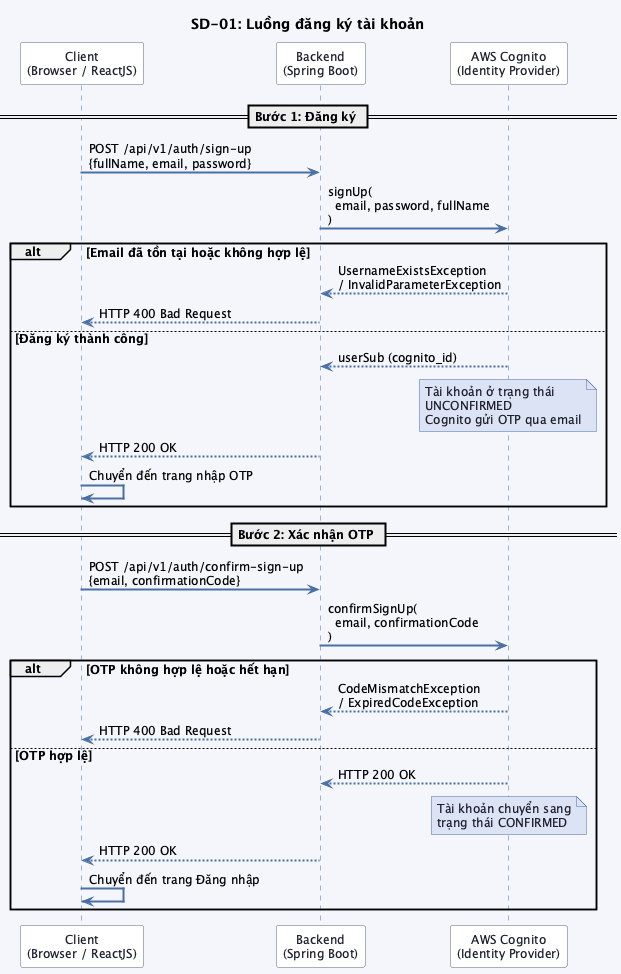
\includegraphics[width=\textwidth, height=0.85\textheight, keepaspectratio]{images/chap3/sequence_sd01.png}
\caption{Biểu đồ tuần tự SD-01: Luồng đăng ký tài khoản}
\label{fig:sequence_sd01}
\end{figure}

% ── SD-02 ─────────────────────────────────────────────────────────────────────

\paragraph{SD-02: Luồng đăng nhập} \mbox{}\\

Backend đóng vai trò trung gian — thay vì Client gọi trực tiếp Cognito, toàn bộ quá trình xác thực được Backend điều phối qua AWS SDK. Sau khi Cognito xác thực thành công, Backend tìm kiếm user trong PostgreSQL theo \texttt{cognito\_id}; nếu chưa tồn tại (lần đăng nhập đầu tiên), Backend tự động tạo mới bản ghi user. JWT nhận được được lưu vào HttpOnly Cookie để bảo vệ khỏi tấn công XSS.

\begin{figure}[H]
\centering
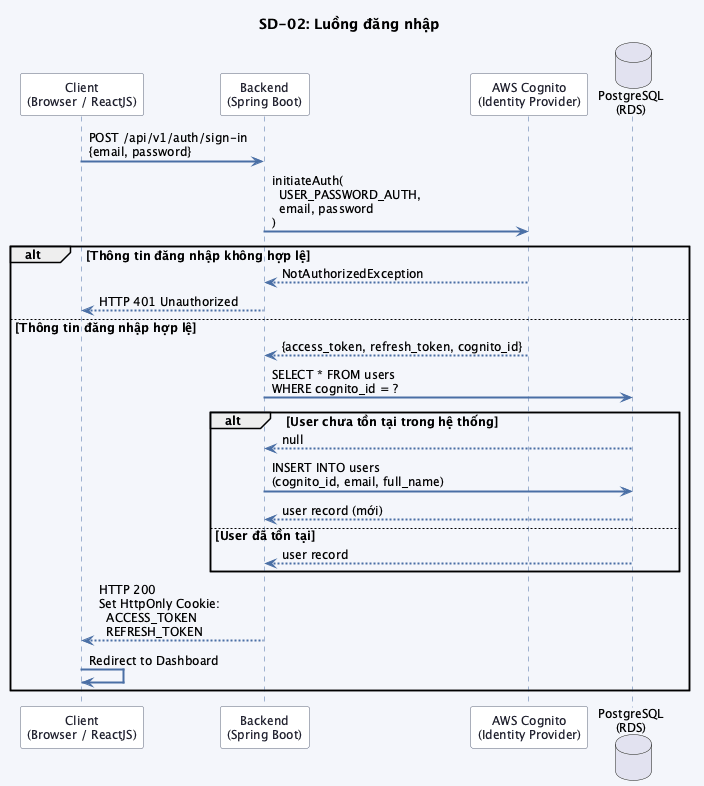
\includegraphics[width=\textwidth, height=0.85\textheight, keepaspectratio]{images/chap3/sequence_sd02.png}
\caption{Biểu đồ tuần tự SD-02: Luồng đăng nhập}
\label{fig:sequence_sd02}
\end{figure}

% ── SD-03 ─────────────────────────────────────────────────────────────────────

\paragraph{SD-03: Luồng tạo Workspace} \mbox{}\\

Workspace là đơn vị tổ chức cấp cao nhất trong hệ thống. Sau khi Backend xác thực JWT, hệ thống thực hiện hai thao tác ghi tuần tự: tạo bản ghi Workspace và tự động ghi nhận người tạo là thành viên với vai trò \texttt{OWNER} trong bảng \texttt{workspace\_members}.

\begin{figure}[H]
\centering
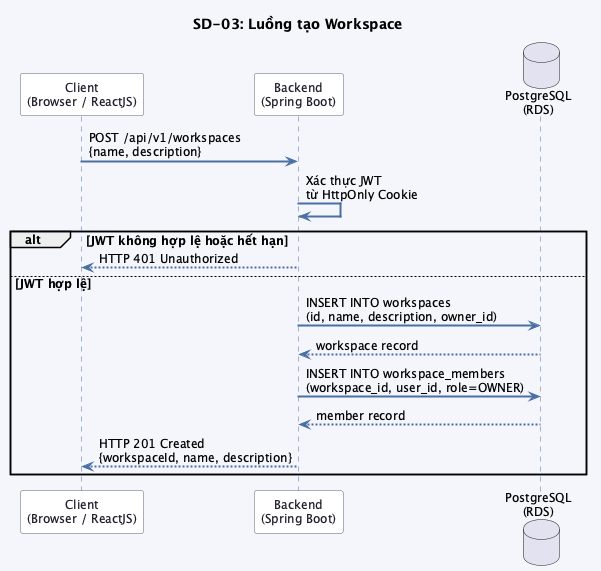
\includegraphics[width=\textwidth, height=0.85\textheight, keepaspectratio]{images/chap3/sequence_sd03.png}
\caption{Biểu đồ tuần tự SD-03: Luồng tạo Workspace}
\label{fig:sequence_sd03}
\end{figure}

% ── SD-04 ─────────────────────────────────────────────────────────────────────

\paragraph{SD-04: Luồng tạo Board} \mbox{}\\

Board được tạo trong phạm vi một Workspace. Backend kiểm tra người dùng có phải thành viên của Workspace trước khi cho phép tạo Board. Sau khi Board được tạo, người tạo được ghi nhận tự động là thành viên Board với vai trò \texttt{OWNER}.

\begin{figure}[H]
\centering
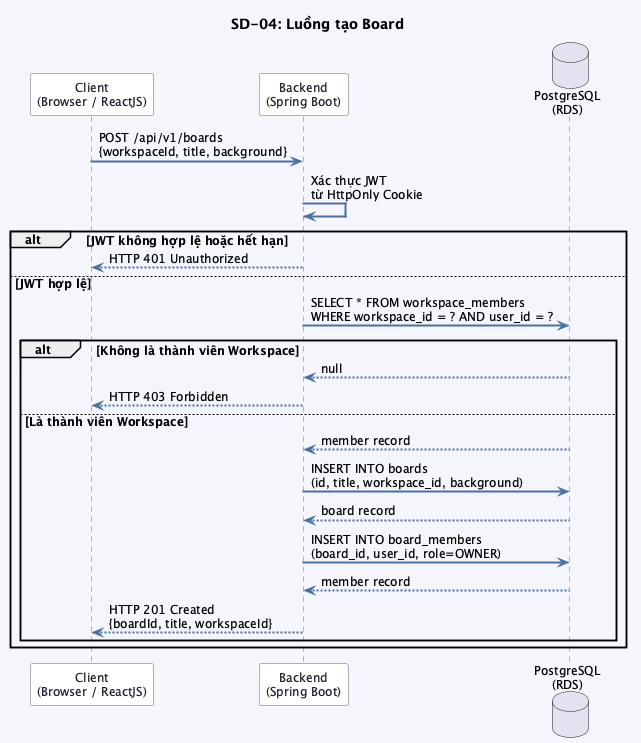
\includegraphics[width=\textwidth, height=0.85\textheight, keepaspectratio]{images/chap3/sequence_sd04.png}
\caption{Biểu đồ tuần tự SD-04: Luồng tạo Board}
\label{fig:sequence_sd04}
\end{figure}

% ── SD-05 ─────────────────────────────────────────────────────────────────────

\paragraph{SD-05: Luồng tạo List} \mbox{}\\

List là các cột trong giao diện Kanban. Backend kiểm tra quyền thành viên Board trước khi thực hiện INSERT. Trường \texttt{position} sử dụng giá trị chuỗi phân số (fractional indexing) để hỗ trợ sắp xếp linh hoạt mà không cần cập nhật lại toàn bộ danh sách.

\begin{figure}[H]
\centering
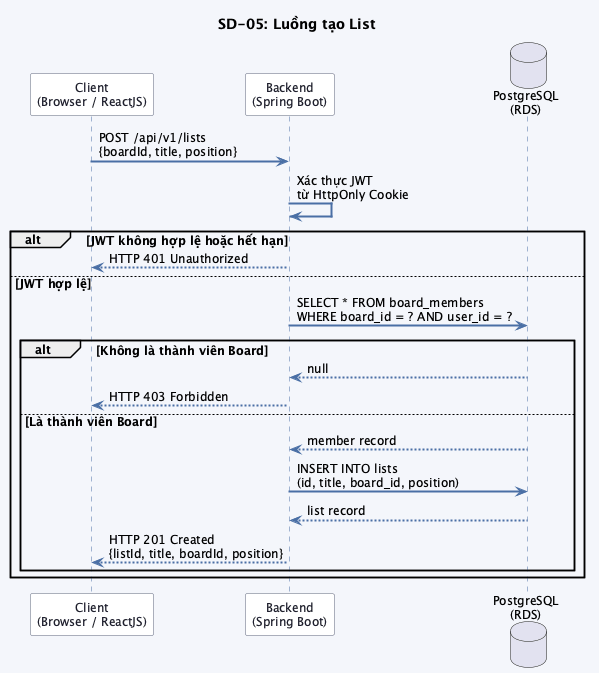
\includegraphics[width=\textwidth, height=0.85\textheight, keepaspectratio]{images/chap3/sequence_sd05.png}
\caption{Biểu đồ tuần tự SD-05: Luồng tạo List}
\label{fig:sequence_sd05}
\end{figure}

% ── SD-06 ─────────────────────────────────────────────────────────────────────

\paragraph{SD-06: Luồng tạo Card} \mbox{}\\

Card là đơn vị công việc cơ bản trong hệ thống. Backend thực hiện hai bước kiểm tra tuần tự trước khi ghi: xác minh List đích tồn tại và xác minh người dùng có quyền trong Board tương ứng. Cơ chế phân quyền này đảm bảo mọi thao tác tạo dữ liệu đều được kiểm soát chặt chẽ.

\begin{figure}[H]
\centering
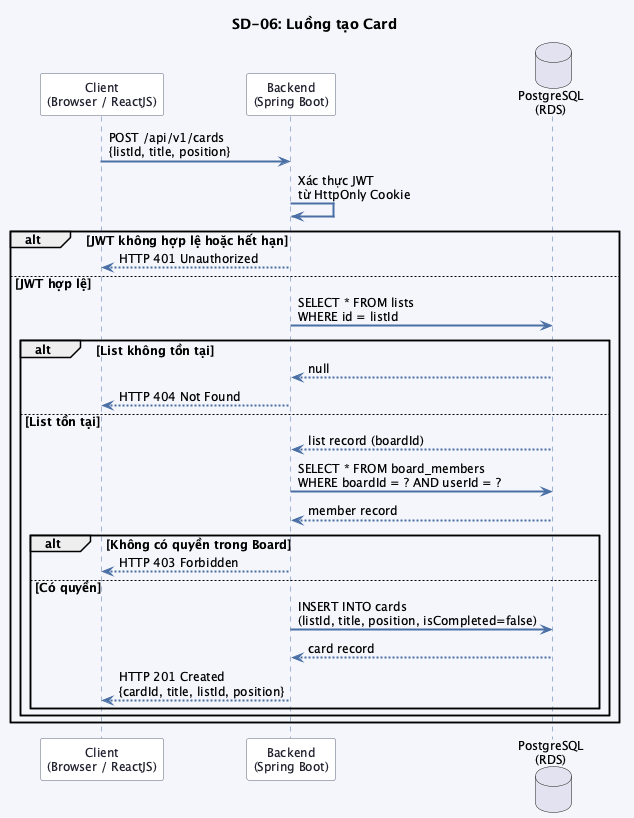
\includegraphics[width=\textwidth, height=0.85\textheight, keepaspectratio]{images/chap3/sequence_sd06.png}
\caption{Biểu đồ tuần tự SD-06: Luồng tạo Card}
\label{fig:sequence_sd06}
\end{figure}

% ── SD-07 ─────────────────────────────────────────────────────────────────────

\paragraph{SD-07: Luồng tải chi tiết Board} \mbox{}\\

Đây là luồng đọc dữ liệu lồng nhau phức tạp nhất trong hệ thống. Backend thực hiện tuần tự: kiểm tra Board tồn tại, kiểm tra quyền truy cập của người dùng, sau đó truy vấn danh sách List và Card theo thứ tự \texttt{position}. Toàn bộ dữ liệu được trả về trong một response để Frontend có thể render ngay giao diện Kanban.

\begin{figure}[H]
\centering
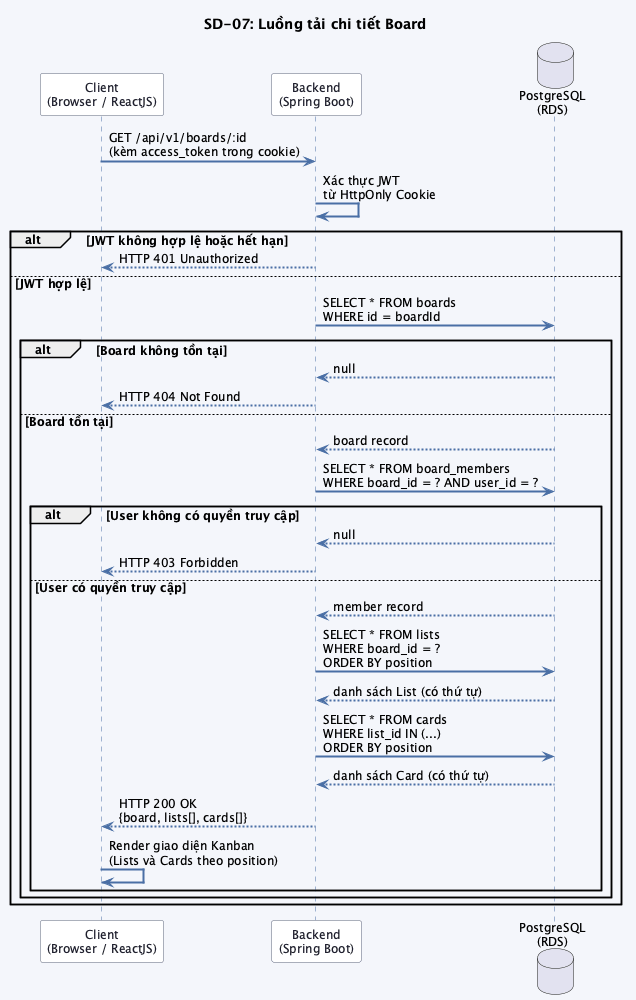
\includegraphics[width=\textwidth, height=0.85\textheight, keepaspectratio]{images/chap3/sequence_sd07.png}
\caption{Biểu đồ tuần tự SD-07: Luồng tải chi tiết Board}
\label{fig:sequence_sd07}
\end{figure}

% ── SD-08 ─────────────────────────────────────────────────────────────────────

\paragraph{SD-08: Luồng thêm thành viên vào Board} \mbox{}\\

Luồng gồm hai giai đoạn: tìm kiếm user theo email và thêm vào Board. Backend xác minh người yêu cầu có quyền trong Board, kiểm tra user đích tồn tại và chưa là thành viên trước khi thực hiện INSERT vào bảng \texttt{board\_members}; nếu đã là thành viên, hệ thống trả về lỗi \texttt{409 Conflict} để tránh trùng lặp.

\begin{figure}[H]
\centering
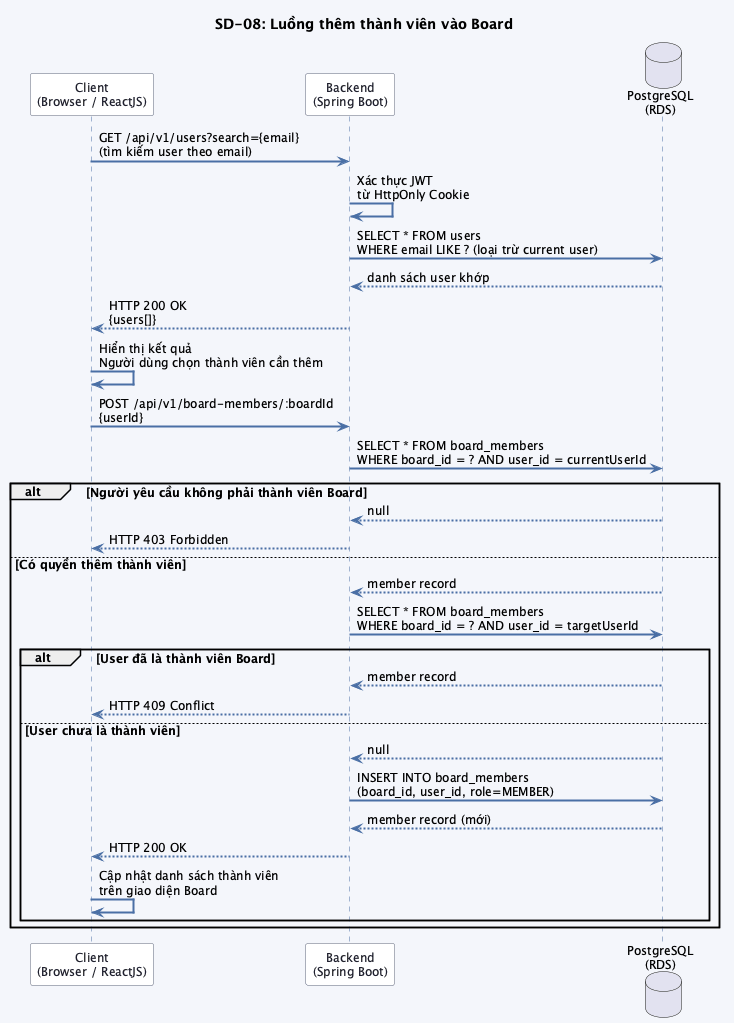
\includegraphics[width=\textwidth, height=0.85\textheight, keepaspectratio]{images/chap3/sequence_sd08.png}
\caption{Biểu đồ tuần tự SD-08: Luồng thêm thành viên vào Board}
\label{fig:sequence_sd08}
\end{figure}

% ── SD-09 ─────────────────────────────────────────────────────────────────────

\paragraph{SD-09: Luồng di chuyển Card (Drag-and-Drop)} \mbox{}\\

Luồng này minh họa kỹ thuật \textbf{optimistic update} — giao diện được cập nhật tức thì ngay khi người dùng kéo thả Card, trước khi nhận phản hồi từ Backend, nhằm tối ưu trải nghiệm người dùng. Nếu yêu cầu cập nhật thất bại (lỗi mạng, hết hạn phiên...), Frontend tự động rollback giao diện về trạng thái trước đó.

\begin{figure}[H]
\centering
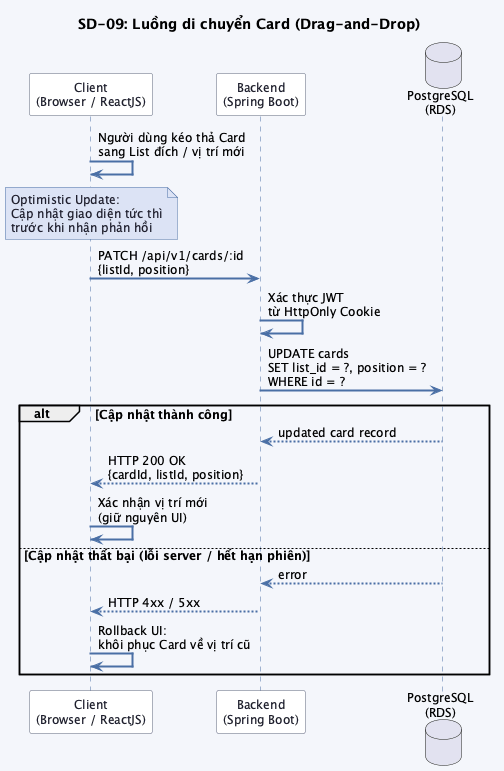
\includegraphics[width=\textwidth, height=0.85\textheight, keepaspectratio]{images/chap3/sequence_sd09.png}
\caption{Biểu đồ tuần tự SD-09: Luồng di chuyển Card (Drag-and-Drop)}
\label{fig:sequence_sd09}
\end{figure}

% ── SD-10 ─────────────────────────────────────────────────────────────────────

\paragraph{SD-10: Luồng di chuyển List (Drag-and-Drop)} \mbox{}\\

Tương tự SD-09, luồng di chuyển List cũng áp dụng kỹ thuật \textbf{optimistic update}. Khi người dùng kéo thả một List sang vị trí khác trong Board, Frontend cập nhật giao diện ngay lập tức trong khi Backend cập nhật trường \texttt{position} vào cơ sở dữ liệu. Nếu thao tác thất bại, UI được rollback về trạng thái ban đầu.

\begin{figure}[H]
\centering
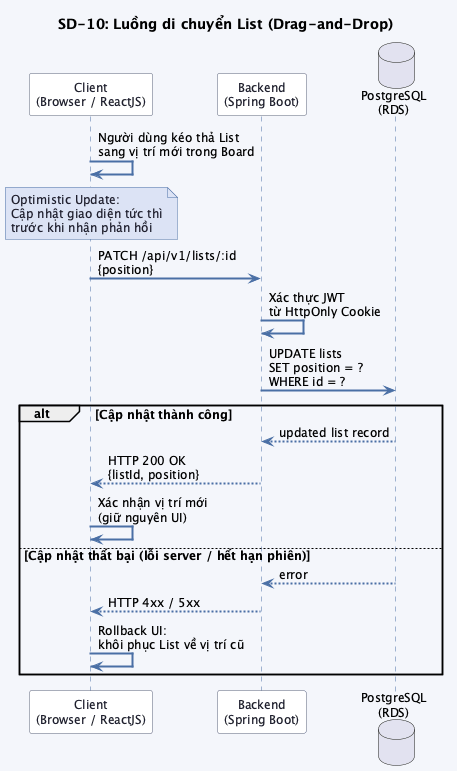
\includegraphics[width=\textwidth, height=0.85\textheight, keepaspectratio]{images/chap3/sequence_sd10.png}
\caption{Biểu đồ tuần tự SD-10: Luồng di chuyển List (Drag-and-Drop)}
\label{fig:sequence_sd10}
\end{figure}

\subsubsection{Thiết kế cơ sở dữ liệu}

Cơ sở dữ liệu của hệ thống Nello sử dụng PostgreSQL, bao gồm 13 bảng được tổ chức thành ba nhóm: bảng tra cứu (lookup tables), bảng tham chiếu (reference tables) và bảng nghiệp vụ (business tables). Khóa chính của các bảng nghiệp vụ sử dụng kiểu UUID để đảm bảo tính duy nhất toàn cục; các bảng tra cứu sử dụng INT. Cơ chế xóa theo tầng (cascade delete) được áp dụng nhất quán theo chuỗi: Workspace $\rightarrow$ Board $\rightarrow$ List $\rightarrow$ Card $\rightarrow$ Checklist $\rightarrow$ ChecklistItem.

\paragraph{Sơ đồ quan hệ} \mbox{}\\

\clearpage
\begin{figure}[p]
    \centering
    \vspace*{-5cm}
    \noindent\makebox[\textwidth][c]{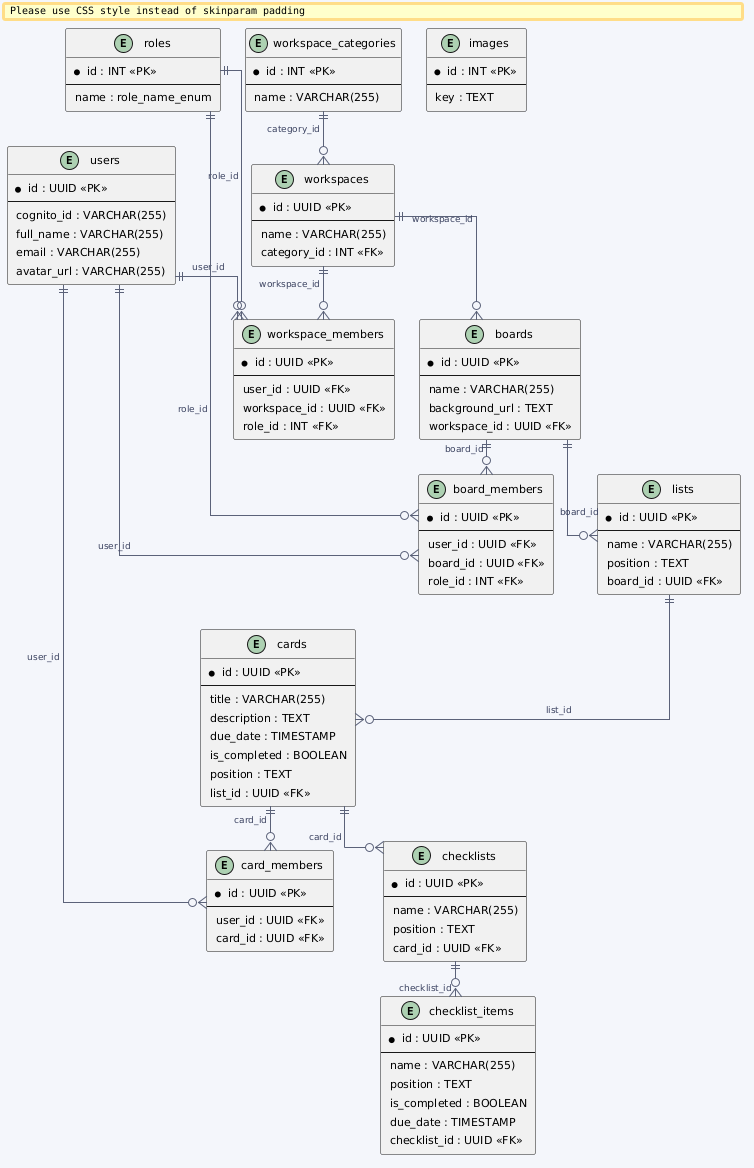
\includegraphics[width=\paperwidth, height=\paperheight, keepaspectratio]{./images/DB_Design.png}}
    \caption{Sơ đồ quan hệ cơ sở dữ liệu hệ thống Nello}
    \label{fig:erd}
\end{figure}
\clearpage

Sơ đồ quan hệ thể hiện toàn bộ cấu trúc dữ liệu của hệ thống với 13 bảng được tổ chức thành ba nhóm chính: bảng tra cứu dùng chung, chuỗi phân cấp nghiệp vụ và bảng trung gian quản lý thành viên. \\

\textbf{Nhóm 1: Bảng tra cứu dùng chung}

\begin{itemize}
    \item \textbf{\texttt{roles} -- \texttt{workspace\_members} / \texttt{board\_members} (1--N):} Bảng \texttt{roles} lưu ba vai trò \texttt{ADMIN}, \texttt{MEMBER}, \texttt{VIEWER}. Cả hai bảng \texttt{workspace\_members} và \texttt{board\_members} đều tham chiếu đến \texttt{roles} qua khóa ngoại \texttt{role\_id}, đảm bảo tính nhất quán của hệ thống phân quyền trong toàn hệ thống.
    \item \textbf{\texttt{workspace\_categories} -- \texttt{workspaces} (1--N):} Mỗi Workspace bắt buộc phải thuộc một loại được định nghĩa sẵn trong \texttt{workspace\_categories} thông qua khóa ngoại \texttt{category\_id}. Một loại Workspace có thể được gán cho nhiều Workspace khác nhau.
    \item \textbf{\texttt{images} -- \texttt{boards}:} Bảng \texttt{images} cung cấp danh sách 8 ảnh nền cố định. Board lưu đường dẫn ảnh được chọn vào trường \texttt{background\_url}.
\end{itemize}

\textbf{Nhóm 2: Chuỗi phân cấp nghiệp vụ} \\

Hệ thống tổ chức dữ liệu theo chuỗi phân cấp từ trên xuống dưới: \texttt{users} $\rightarrow$ \texttt{workspaces} $\rightarrow$ \texttt{boards} $\rightarrow$ \texttt{lists} $\rightarrow$ \texttt{cards} $\rightarrow$ \texttt{checklists} $\rightarrow$ \texttt{checklist\_items}. Mỗi cấp đều áp dụng ràng buộc \texttt{ON DELETE CASCADE}, nghĩa là khi một bản ghi ở cấp trên bị xóa, toàn bộ dữ liệu ở các cấp dưới sẽ bị xóa theo.

\begin{itemize}
    \item \textbf{\texttt{users} -- \texttt{workspaces} (1--N):} Mỗi Workspace được tạo bởi một người dùng xác định qua \texttt{created\_by}. Trường \texttt{updated\_by} ghi lại người thực hiện cập nhật gần nhất, cả hai đều là khóa ngoại tham chiếu \texttt{users.id}.
    \item \textbf{\texttt{workspaces} -- \texttt{boards} (1--N):} Mỗi Board thuộc về đúng một Workspace qua khóa ngoại \texttt{workspace\_id}. Khi Workspace bị xóa, toàn bộ Board bên trong bị xóa theo (CASCADE).
    \item \textbf{\texttt{boards} -- \texttt{lists} (1--N):} Mỗi List thuộc về đúng một Board qua khóa ngoại \texttt{board\_id}. Thứ tự hiển thị của các List được quản lý qua trường \texttt{position} theo thuật toán fractional indexing.
    \item \textbf{\texttt{lists} -- \texttt{cards} (1--N):} Mỗi Card thuộc về đúng một List qua khóa ngoại \texttt{list\_id}. Card có thể được di chuyển giữa các List trong cùng Board bằng cách cập nhật \texttt{list\_id}.
    \item \textbf{\texttt{cards} -- \texttt{checklists} (1--N):} Mỗi Checklist gắn với một Card duy nhất qua khóa ngoại \texttt{card\_id}. Một Card có thể chứa nhiều Checklist, thứ tự hiển thị được quản lý qua \texttt{position}.
    \item \textbf{\texttt{checklists} -- \texttt{checklist\_items} (1--N):} Mỗi ChecklistItem thuộc về đúng một Checklist qua khóa ngoại \texttt{checklist\_id}. Tỷ lệ hoàn thành của Checklist được tính dựa trên số lượng item có \texttt{is\_completed = true}.
\end{itemize}

\textbf{Nhóm 3: Quan hệ nhiều--nhiều quản lý thành viên}

\begin{itemize}
    \item \textbf{\texttt{users} -- \texttt{workspaces} qua \texttt{workspace\_members} (N--N):} Một người dùng có thể là thành viên của nhiều Workspace và một Workspace có thể có nhiều thành viên. Bảng trung gian \texttt{workspace\_members} lưu cặp (\texttt{user\_id}, \texttt{workspace\_id}) cùng với \texttt{role\_id} xác định quyền hạn. Ràng buộc UNIQUE trên cặp này đảm bảo mỗi người dùng chỉ có một vai trò duy nhất trong mỗi Workspace.
    \item \textbf{\texttt{users} -- \texttt{boards} qua \texttt{board\_members} (N--N):} Bảng \texttt{board\_members} quản lý danh sách thành viên trong từng Board kèm vai trò tương ứng, độc lập với danh sách thành viên Workspace. Một người dùng bất kỳ có thể được thêm vào Board mà không cần phải là thành viên của Workspace chứa Board đó. Ràng buộc UNIQUE trên cặp (\texttt{user\_id}, \texttt{board\_id}) ngăn chặn trùng lặp.
    \item \textbf{\texttt{users} -- \texttt{cards} qua \texttt{card\_members} (N--N):} Bảng \texttt{card\_members} ghi nhận các thành viên được gán làm người phụ trách cho Card. Không có trường \texttt{role\_id} vì quan hệ này chỉ mang ý nghĩa gán trách nhiệm, không phân quyền. Ràng buộc UNIQUE trên cặp (\texttt{user\_id}, \texttt{card\_id}) đảm bảo mỗi thành viên chỉ được gán một lần.
\end{itemize}

\paragraph{Đặc tả bảng} \mbox{}\\

% ------------------------------------------------------------------
\paragraph{Bảng \texttt{roles}} \mbox{}\\

\textbf{a. Mô tả}

Bảng \texttt{roles} lưu trữ các vai trò của thành viên trong hệ thống. Đây là bảng tra cứu dùng chung cho cả Workspace và Board. \\

\textbf{b. Cấu trúc bảng}

\begin{table}[H]
\centering
\begin{tabular}{|p{3cm}|p{3.5cm}|p{3.5cm}|p{4cm}|}
\hline
\textbf{Tên trường} & \textbf{Kiểu dữ liệu} & \textbf{Ràng buộc} & \textbf{Ý nghĩa} \\
\hline
\texttt{id} & INT & Khóa chính & Mã vai trò. \\
\hline
\texttt{name} & role\_name\_enum & NOT NULL, UNIQUE & Tên vai trò. \\
\hline
\end{tabular}
\caption{Bảng \texttt{roles}}
\label{tab:db_roles}
\end{table}

\textbf{c. Ghi chú}

Trường \texttt{name} thuộc kiểu liệt kê \texttt{role\_name\_enum} nhận một trong ba giá trị: \texttt{ADMIN}, \texttt{MEMBER}, \texttt{VIEWER}. Dữ liệu được nạp sẵn khi khởi tạo hệ thống.

% ------------------------------------------------------------------
\paragraph{Bảng \texttt{images}} \mbox{}\\

\textbf{a. Mô tả}

Bảng \texttt{images} cung cấp danh sách 8 ảnh nền cố định cho Board. Người dùng chọn một trong các ảnh này khi tạo hoặc cập nhật Board. \\

\textbf{b. Cấu trúc bảng}

\begin{table}[H]
\centering
\begin{tabular}{|p{3cm}|p{3.5cm}|p{3.5cm}|p{4cm}|}
\hline
\textbf{Tên trường} & \textbf{Kiểu dữ liệu} & \textbf{Ràng buộc} & \textbf{Ý nghĩa} \\
\hline
\texttt{id} & INT & Khóa chính & Mã ảnh nền. \\
\hline
\texttt{key} & TEXT & NOT NULL & Đường dẫn tương đối đến tệp ảnh nền. \\
\hline
\end{tabular}
\caption{Bảng \texttt{images}}
\label{tab:db_images}
\end{table}

% ------------------------------------------------------------------
\paragraph{Bảng \texttt{workspace\_categories}} \mbox{}\\

\textbf{a. Mô tả}

Bảng \texttt{workspace\_categories} lưu danh sách các loại Workspace để phân loại không gian làm việc khi tạo mới.\\

\textbf{b. Cấu trúc bảng}

\begin{table}[H]
\centering
\begin{tabular}{|p{3cm}|p{3.5cm}|p{3.5cm}|p{4cm}|}
\hline
\textbf{Tên trường} & \textbf{Kiểu dữ liệu} & \textbf{Ràng buộc} & \textbf{Ý nghĩa} \\
\hline
\texttt{id} & INT & Khóa chính & Mã loại Workspace. \\
\hline
\texttt{name} & VARCHAR(255) & NOT NULL & Tên loại Workspace. \\
\hline
\end{tabular}
\caption{Bảng \texttt{workspace\_categories}}
\label{tab:db_workspace_categories}
\end{table}

\textbf{c. Ghi chú}

Hệ thống cung cấp sẵn 8 loại: Sales CRM, Education, Human Resources, Operation, Marketing, IT, Small Business, Other.

% ------------------------------------------------------------------
\paragraph{Bảng \texttt{users}} \mbox{}\\

\textbf{a. Mô tả}

Bảng \texttt{users} lưu thông tin người dùng trong hệ thống. Thông tin xác thực được quản lý bởi Amazon Cognito; trường \texttt{cognito\_id} là liên kết giữa hệ thống nội bộ và Cognito User Pool.\\

\textbf{b. Cấu trúc bảng}

\begin{table}[H]
\centering
\begin{tabular}{|p{3cm}|p{3.5cm}|p{3.5cm}|p{4cm}|}
\hline
\textbf{Tên trường} & \textbf{Kiểu dữ liệu} & \textbf{Ràng buộc} & \textbf{Ý nghĩa} \\
\hline
\texttt{id} & UUID & Khóa chính & Mã định danh nội bộ. \\
\hline
\texttt{cognito\_id} & VARCHAR(255) & NOT NULL, UNIQUE & Mã định danh từ Amazon Cognito. \\
\hline
\texttt{full\_name} & VARCHAR(255) & NOT NULL & Họ tên đầy đủ. \\
\hline
\texttt{email} & VARCHAR(255) & NOT NULL, UNIQUE & Địa chỉ email. \\
\hline
\texttt{avatar\_url} & VARCHAR(255) & NULL & Đường dẫn ảnh đại diện. \\
\hline
\texttt{bio} & TEXT & NULL & Giới thiệu bản thân. \\
\hline
\texttt{phone} & VARCHAR(255) & NULL & Số điện thoại. \\
\hline
\texttt{address} & VARCHAR(255) & NULL & Địa chỉ. \\
\hline
\texttt{deleted\_at} & TIMESTAMP & NULL & Thời điểm xóa mềm tài khoản. \\
\hline
\texttt{created\_at} & TIMESTAMP & NOT NULL, DEFAULT NOW() & Thời điểm tạo bản ghi. \\
\hline
\texttt{updated\_at} & TIMESTAMP & NOT NULL, DEFAULT NOW() & Thời điểm cập nhật gần nhất. \\
\hline
\end{tabular}
\caption{Bảng \texttt{users}}
\label{tab:db_users}
\end{table}

% ------------------------------------------------------------------
\paragraph{Bảng \texttt{workspaces}} \mbox{}\\

\textbf{a. Mô tả}

Bảng \texttt{workspaces} lưu thông tin các không gian làm việc. Đây là đơn vị tổ chức cấp cao nhất trong hệ thống, chứa nhiều Board bên trong.\\

\textbf{b. Cấu trúc bảng}

\begin{table}[H]
\centering
\begin{tabular}{|p{3cm}|p{3.5cm}|p{3.5cm}|p{4cm}|}
\hline
\textbf{Tên trường} & \textbf{Kiểu dữ liệu} & \textbf{Ràng buộc} & \textbf{Ý nghĩa} \\
\hline
\texttt{id} & UUID & Khóa chính & Mã định danh. \\
\hline
\texttt{name} & VARCHAR(255) & NOT NULL & Tên Workspace. \\
\hline
\texttt{description} & VARCHAR(255) & NULL & Mô tả Workspace. \\
\hline
\texttt{category\_id} & INT & NOT NULL, FK $\rightarrow$ workspace\_categories & Loại Workspace. \\
\hline
\texttt{created\_by} & UUID & NOT NULL, FK $\rightarrow$ users & Người tạo Workspace. \\
\hline
\texttt{updated\_by} & UUID & NULL, FK $\rightarrow$ users & Người cập nhật gần nhất. \\
\hline
\texttt{created\_at} & TIMESTAMP & NOT NULL, DEFAULT NOW() & Thời điểm tạo bản ghi. \\
\hline
\texttt{updated\_at} & TIMESTAMP & NOT NULL, DEFAULT NOW() & Thời điểm cập nhật gần nhất. \\
\hline
\end{tabular}
\caption{Bảng \texttt{workspaces}}
\label{tab:db_workspaces}
\end{table}

% ------------------------------------------------------------------
\paragraph{Bảng \texttt{workspace\_members}} \mbox{}\\

\textbf{a. Mô tả}

Bảng \texttt{workspace\_members} là bảng trung gian thể hiện quan hệ nhiều--nhiều giữa người dùng và Workspace. Mỗi bản ghi xác định một thành viên trong một Workspace cùng vai trò tương ứng.\\

\textbf{b. Cấu trúc bảng}

\begin{table}[H]
\centering
\begin{tabular}{|p{3cm}|p{3.5cm}|p{3.5cm}|p{4cm}|}
\hline
\textbf{Tên trường} & \textbf{Kiểu dữ liệu} & \textbf{Ràng buộc} & \textbf{Ý nghĩa} \\
\hline
\texttt{id} & UUID & Khóa chính & Mã định danh. \\
\hline
\texttt{user\_id} & UUID & NOT NULL, FK $\rightarrow$ users & Thành viên được thêm vào Workspace. \\
\hline
\texttt{workspace\_id} & UUID & NOT NULL, FK $\rightarrow$ workspaces & Workspace chứa thành viên. \\
\hline
\texttt{role\_id} & INT & NOT NULL, FK $\rightarrow$ roles & Vai trò trong Workspace. \\
\hline
\texttt{created\_by} & UUID & NOT NULL, FK $\rightarrow$ users & Người thêm thành viên. \\
\hline
\texttt{created\_at} & TIMESTAMP & NOT NULL, DEFAULT NOW() & Thời điểm thêm thành viên. \\
\hline
\end{tabular}
\caption{Bảng \texttt{workspace\_members}}
\label{tab:db_workspace_members}
\end{table}

\textbf{c. Ghi chú}

Ràng buộc UNIQUE trên cặp (\texttt{user\_id}, \texttt{workspace\_id}) đảm bảo mỗi người dùng chỉ có một vai trò duy nhất trong một Workspace. Khi Workspace hoặc User bị xóa, bản ghi liên quan sẽ bị xóa theo (ON DELETE CASCADE).

% ------------------------------------------------------------------
\paragraph{Bảng \texttt{boards}} \mbox{}\\

\textbf{a. Mô tả}

Bảng \texttt{boards} lưu thông tin các bảng công việc bên trong Workspace. Mỗi Board có thể có ảnh nền riêng được chọn từ bảng \texttt{images}.\\

\textbf{b. Cấu trúc bảng}

\begin{table}[H]
\centering
\begin{tabular}{|p{3cm}|p{3.5cm}|p{3.5cm}|p{4cm}|}
\hline
\textbf{Tên trường} & \textbf{Kiểu dữ liệu} & \textbf{Ràng buộc} & \textbf{Ý nghĩa} \\
\hline
\texttt{id} & UUID & Khóa chính & Mã định danh. \\
\hline
\texttt{name} & VARCHAR(255) & NOT NULL & Tên Board. \\
\hline
\texttt{background\_url} & TEXT & NULL & Đường dẫn ảnh nền Board. \\
\hline
\texttt{workspace\_id} & UUID & NOT NULL, FK $\rightarrow$ workspaces, CASCADE & Workspace chứa Board. \\
\hline
\texttt{created\_by} & UUID & NOT NULL, FK $\rightarrow$ users & Người tạo Board. \\
\hline
\texttt{updated\_by} & UUID & NULL, FK $\rightarrow$ users & Người cập nhật gần nhất. \\
\hline
\texttt{created\_at} & TIMESTAMP & NOT NULL, DEFAULT NOW() & Thời điểm tạo bản ghi. \\
\hline
\texttt{updated\_at} & TIMESTAMP & NOT NULL, DEFAULT NOW() & Thời điểm cập nhật gần nhất. \\
\hline
\end{tabular}
\caption{Bảng \texttt{boards}}
\label{tab:db_boards}
\end{table}

% ------------------------------------------------------------------
\paragraph{Bảng \texttt{board\_members}} \mbox{}\\

\textbf{a. Mô tả}

Bảng \texttt{board\_members} là bảng trung gian thể hiện quan hệ nhiều--nhiều giữa người dùng và Board. Mỗi thành viên trong Board có một vai trò xác định quyền thao tác trong Board đó.\\

\textbf{b. Cấu trúc bảng}

\begin{table}[H]
\centering
\begin{tabular}{|p{3cm}|p{3.5cm}|p{3.5cm}|p{4cm}|}
\hline
\textbf{Tên trường} & \textbf{Kiểu dữ liệu} & \textbf{Ràng buộc} & \textbf{Ý nghĩa} \\
\hline
\texttt{id} & UUID & Khóa chính & Mã định danh. \\
\hline
\texttt{user\_id} & UUID & NOT NULL, FK $\rightarrow$ users & Thành viên được thêm vào Board. \\
\hline
\texttt{board\_id} & UUID & NOT NULL, FK $\rightarrow$ boards, CASCADE & Board chứa thành viên. \\
\hline
\texttt{role\_id} & INT & NOT NULL, FK $\rightarrow$ roles & Vai trò trong Board. \\
\hline
\texttt{created\_by} & UUID & NOT NULL, FK $\rightarrow$ users & Người thêm thành viên. \\
\hline
\texttt{created\_at} & TIMESTAMP & NOT NULL, DEFAULT NOW() & Thời điểm thêm thành viên. \\
\hline
\end{tabular}
\caption{Bảng \texttt{board\_members}}
\label{tab:db_board_members}
\end{table}

\textbf{c. Ghi chú}

Ràng buộc UNIQUE trên cặp (\texttt{user\_id}, \texttt{board\_id}) đảm bảo mỗi người dùng chỉ có một vai trò duy nhất trong một Board. Danh sách thành viên Board hoàn toàn độc lập với danh sách thành viên Workspace — người dùng có thể được thêm trực tiếp vào Board mà không cần thuộc Workspace chứa Board đó.

% ------------------------------------------------------------------
\paragraph{Bảng \texttt{lists}} \mbox{}\\

\textbf{a. Mô tả}

Bảng \texttt{lists} lưu các cột trạng thái (List) bên trong Board theo mô hình Kanban. Thứ tự hiển thị của List được quản lý qua trường \texttt{position}.\\

\textbf{b. Cấu trúc bảng}

\begin{table}[H]
\centering
\begin{tabular}{|p{3cm}|p{3.5cm}|p{3.5cm}|p{4cm}|}
\hline
\textbf{Tên trường} & \textbf{Kiểu dữ liệu} & \textbf{Ràng buộc} & \textbf{Ý nghĩa} \\
\hline
\texttt{id} & UUID & Khóa chính & Mã định danh. \\
\hline
\texttt{name} & VARCHAR(255) & NOT NULL & Tên List. \\
\hline
\texttt{position} & TEXT & NOT NULL & Giá trị vị trí dùng để sắp xếp và kéo thả. \\
\hline
\texttt{board\_id} & UUID & NOT NULL, FK $\rightarrow$ boards, CASCADE & Board chứa List. \\
\hline
\texttt{created\_by} & UUID & NOT NULL, FK $\rightarrow$ users & Người tạo List. \\
\hline
\texttt{updated\_by} & UUID & NULL, FK $\rightarrow$ users & Người cập nhật gần nhất. \\
\hline
\texttt{created\_at} & TIMESTAMP & NOT NULL, DEFAULT NOW() & Thời điểm tạo bản ghi. \\
\hline
\texttt{updated\_at} & TIMESTAMP & NOT NULL, DEFAULT NOW() & Thời điểm cập nhật gần nhất. \\
\hline
\end{tabular}
\caption{Bảng \texttt{lists}}
\label{tab:db_lists}
\end{table}

\textbf{c. Ghi chú}

Trường \texttt{position} sử dụng kiểu TEXT thay vì INT để tránh phải đánh lại chỉ số toàn bộ khi chèn phần tử vào giữa. Thuật toán fractional indexing được áp dụng để tính giá trị position khi kéo thả.

% ------------------------------------------------------------------
\paragraph{Bảng \texttt{cards}} \mbox{}\\

\textbf{a. Mô tả}

Bảng \texttt{cards} là bảng trung tâm của hệ thống, lưu toàn bộ thông tin về các thẻ công việc. Mỗi Card thuộc về một List và có thể được gán thành viên phụ trách, thiết lập ngày bắt đầu và ngày đến hạn.\\

\textbf{b. Cấu trúc bảng}

\begin{table}[H]
\centering
\begin{tabular}{|p{3cm}|p{3.5cm}|p{3.5cm}|p{4cm}|}
\hline
\textbf{Tên trường} & \textbf{Kiểu dữ liệu} & \textbf{Ràng buộc} & \textbf{Ý nghĩa} \\
\hline
\texttt{id} & UUID & Khóa chính & Mã định danh. \\
\hline
\texttt{title} & VARCHAR(255) & NOT NULL & Tiêu đề Card. \\
\hline
\texttt{description} & TEXT & NULL & Mô tả chi tiết. \\
\hline
\texttt{start\_date} & TIMESTAMP & NULL & Ngày bắt đầu. \\
\hline
\texttt{due\_date} & TIMESTAMP & NULL & Ngày đến hạn hoàn thành. \\
\hline
\texttt{is\_completed} & BOOLEAN & NOT NULL, DEFAULT FALSE & Trạng thái hoàn thành. \\
\hline
\texttt{position} & TEXT & NOT NULL & Giá trị vị trí dùng để sắp xếp và kéo thả. \\
\hline
\texttt{list\_id} & UUID & NOT NULL, FK $\rightarrow$ lists, CASCADE & List chứa Card. \\
\hline
\texttt{created\_by} & UUID & NOT NULL, FK $\rightarrow$ users & Người tạo Card. \\
\hline
\texttt{updated\_by} & UUID & NULL, FK $\rightarrow$ users & Người cập nhật gần nhất. \\
\hline
\texttt{created\_at} & TIMESTAMP & NOT NULL, DEFAULT NOW() & Thời điểm tạo bản ghi. \\
\hline
\texttt{updated\_at} & TIMESTAMP & NOT NULL, DEFAULT NOW() & Thời điểm cập nhật gần nhất. \\
\hline
\end{tabular}
\caption{Bảng \texttt{cards}}
\label{tab:db_cards}
\end{table}

% ------------------------------------------------------------------
\paragraph{Bảng \texttt{card\_members}} \mbox{}\\

\textbf{a. Mô tả}

Bảng \texttt{card\_members} là bảng trung gian thể hiện quan hệ nhiều--nhiều giữa người dùng và Card. Mỗi bản ghi xác định một thành viên được gán làm người phụ trách cho Card.\\

\textbf{b. Cấu trúc bảng}

\begin{table}[H]
\centering
\begin{tabular}{|p{3cm}|p{3.5cm}|p{3.5cm}|p{4cm}|}
\hline
\textbf{Tên trường} & \textbf{Kiểu dữ liệu} & \textbf{Ràng buộc} & \textbf{Ý nghĩa} \\
\hline
\texttt{id} & UUID & Khóa chính & Mã định danh. \\
\hline
\texttt{user\_id} & UUID & NOT NULL, FK $\rightarrow$ users & Thành viên được gán vào Card. \\
\hline
\texttt{card\_id} & UUID & NOT NULL, FK $\rightarrow$ cards, CASCADE & Card được gán thành viên. \\
\hline
\texttt{created\_by} & UUID & NOT NULL, FK $\rightarrow$ users & Người gán thành viên. \\
\hline
\texttt{created\_at} & TIMESTAMP & NOT NULL, DEFAULT NOW() & Thời điểm gán thành viên. \\
\hline
\end{tabular}
\caption{Bảng \texttt{card\_members}}
\label{tab:db_card_members}
\end{table}

\textbf{c. Ghi chú}

Ràng buộc UNIQUE trên cặp (\texttt{user\_id}, \texttt{card\_id}) đảm bảo mỗi thành viên chỉ được gán một lần cho mỗi Card.

% ------------------------------------------------------------------
\paragraph{Bảng \texttt{checklists}} \mbox{}\\

\textbf{a. Mô tả}

Bảng \texttt{checklists} lưu các danh sách kiểm tra bên trong Card. Mỗi Card có thể có nhiều Checklist, mỗi Checklist lại chứa nhiều ChecklistItem.\\

\textbf{b. Cấu trúc bảng}

\begin{table}[H]
\centering
\begin{tabular}{|p{3cm}|p{3.5cm}|p{3.5cm}|p{4cm}|}
\hline
\textbf{Tên trường} & \textbf{Kiểu dữ liệu} & \textbf{Ràng buộc} & \textbf{Ý nghĩa} \\
\hline
\texttt{id} & UUID & Khóa chính & Mã định danh. \\
\hline
\texttt{name} & VARCHAR(255) & NOT NULL & Tên Checklist. \\
\hline
\texttt{position} & TEXT & NOT NULL & Vị trí hiển thị trong Card. \\
\hline
\texttt{card\_id} & UUID & NOT NULL, FK $\rightarrow$ cards, CASCADE & Card chứa Checklist. \\
\hline
\texttt{created\_by} & UUID & NOT NULL, FK $\rightarrow$ users & Người tạo Checklist. \\
\hline
\texttt{updated\_by} & UUID & NULL, FK $\rightarrow$ users & Người cập nhật gần nhất. \\
\hline
\texttt{created\_at} & TIMESTAMP & NOT NULL, DEFAULT NOW() & Thời điểm tạo bản ghi. \\
\hline
\texttt{updated\_at} & TIMESTAMP & NOT NULL, DEFAULT NOW() & Thời điểm cập nhật gần nhất. \\
\hline
\end{tabular}
\caption{Bảng \texttt{checklists}}
\label{tab:db_checklists}
\end{table}

% ------------------------------------------------------------------
\paragraph{Bảng \texttt{checklist\_items}} \mbox{}\\

\textbf{a. Mô tả}

Bảng \texttt{checklist\_items} lưu các hạng mục công việc con bên trong Checklist. Mỗi hạng mục có trạng thái hoàn thành riêng và có thể thiết lập ngày đến hạn độc lập. Frontend sử dụng tỷ lệ \texttt{is\_completed} của các item để hiển thị thanh tiến độ (progress bar).\\

\textbf{b. Cấu trúc bảng}

\begin{table}[H]
\centering
\begin{tabular}{|p{3cm}|p{3.5cm}|p{3.5cm}|p{4cm}|}
\hline
\textbf{Tên trường} & \textbf{Kiểu dữ liệu} & \textbf{Ràng buộc} & \textbf{Ý nghĩa} \\
\hline
\texttt{id} & UUID & Khóa chính & Mã định danh. \\
\hline
\texttt{name} & VARCHAR(255) & NOT NULL & Tên hạng mục. \\
\hline
\texttt{position} & TEXT & NOT NULL & Vị trí hiển thị trong Checklist. \\
\hline
\texttt{is\_completed} & BOOLEAN & NOT NULL, DEFAULT FALSE & Trạng thái hoàn thành của hạng mục. \\
\hline
\texttt{due\_date} & TIMESTAMP & NULL & Thời hạn riêng của hạng mục. \\
\hline
\texttt{checklist\_id} & UUID & NOT NULL, FK $\rightarrow$ checklists, CASCADE & Checklist chứa hạng mục. \\
\hline
\texttt{created\_by} & UUID & NOT NULL, FK $\rightarrow$ users & Người tạo hạng mục. \\
\hline
\texttt{updated\_by} & UUID & NULL, FK $\rightarrow$ users & Người cập nhật gần nhất. \\
\hline
\texttt{created\_at} & TIMESTAMP & NOT NULL, DEFAULT NOW() & Thời điểm tạo bản ghi. \\
\hline
\texttt{updated\_at} & TIMESTAMP & NOT NULL, DEFAULT NOW() & Thời điểm cập nhật gần nhất. \\
\hline
\end{tabular}
\caption{Bảng \texttt{checklist\_items}}
\label{tab:db_checklist_items}
\end{table}

\textbf{c. Ghi chú}

Ràng buộc CHECK trên trường \texttt{is\_completed} đảm bảo chỉ nhận hai giá trị hợp lệ: \texttt{true} hoặc \texttt{false}.


\subsubsection{Thiết kế giao diện}

\textbf{TODO: Bổ sung nội dung}

\clearpage

\section{CHƯƠNG 4: TRIỂN KHAI VÀ KẾT QUẢ}

\subsection{Các chức năng đã hoàn thành}

Sau 8 tuần thực hiện (từ 30/03 đến 24/05/2026), hệ thống Nello đã hoàn thành \textbf{27/31 chức năng} yêu cầu, đạt tỷ lệ \textbf{87,1\%}.

\begin{longtable}{|c|p{2.5cm}|p{9cm}|}
\hline
\textbf{STT} & \textbf{Mã FR} & \textbf{Tên chức năng} \\
\hline
\endfirsthead
\hline
\textbf{STT} & \textbf{Mã FR} & \textbf{Tên chức năng} \\
\hline
\endhead
\hline
\endfoot

\multicolumn{3}{|l|}{\cellcolor{gray!20}\textbf{Nhóm 1: Xác thực và quản lý tài khoản}} \\
\hline
1 & FR-01 & Đăng ký tài khoản \\
\hline
2 & FR-02 & Xác nhận email \\
\hline
3 & FR-03 & Đăng nhập \\
\hline
4 & FR-04 & Đăng xuất \\
\hline
5 & FR-05 & Làm mới phiên làm việc \\
\hline
6 & FR-32 & Đổi mật khẩu \\
\hline
7 & FR-33 & Cập nhật hồ sơ cá nhân \\
\hline
\multicolumn{3}{|l|}{\cellcolor{gray!20}\textbf{Nhóm 2: Quản lý Workspace}} \\
\hline
8 & FR-06 & Tạo Workspace \\
\hline
9 & FR-07 & Xem danh sách Workspace \\
\hline
10 & FR-09 & Quản lý thành viên Workspace \\
\hline
\multicolumn{3}{|l|}{\cellcolor{gray!20}\textbf{Nhóm 3: Quản lý Board}} \\
\hline
11 & FR-10 & Tạo Board \\
\hline
12 & FR-11 & Xem Board \\
\hline
13 & FR-13 & Quản lý thành viên Board \\
\hline
\multicolumn{3}{|l|}{\cellcolor{gray!20}\textbf{Nhóm 4: Quản lý List}} \\
\hline
14 & FR-14 & Tạo List \\
\hline
15 & FR-15 & Cập nhật List \\
\hline
16 & FR-16 & Xóa List \\
\hline
\multicolumn{3}{|l|}{\cellcolor{gray!20}\textbf{Nhóm 5: Quản lý Card}} \\
\hline
17 & FR-17 & Tạo Card \\
\hline
18 & FR-18 & Xem chi tiết Card \\
\hline
19 & FR-19 & Cập nhật Card \\
\hline
20 & FR-20 & Xóa Card \\
\hline
21 & FR-22 & Gán thành viên vào Card \\
\hline
\multicolumn{3}{|l|}{\cellcolor{gray!20}\textbf{Nhóm 6: Kéo thả (Drag and Drop)}} \\
\hline
22 & FR-23 & Kéo thả Card \\
\hline
23 & FR-24 & Kéo thả List trong Board \\
\hline
\multicolumn{3}{|l|}{\cellcolor{gray!20}\textbf{Nhóm 7: Quản lý Checklist}} \\
\hline
24 & FR-26 & Tạo Checklist \\
\hline
25 & FR-27 & Cập nhật Checklist \\
\hline
26 & FR-28 & Xóa Checklist \\
\hline
27 & FR-29 & Quản lý ChecklistItem \\
\hline
\caption{Danh sách chức năng đã hoàn thành (27/31 — 87,1\%)}
\label{tab:done_all}
\end{longtable}

\subsection{Kết quả đạt được}

\subsubsection{Thống kê tổng quát}

\begin{table}[H]
\centering
\begin{tabular}{|p{6cm}|p{8cm}|}
\hline
\textbf{Hạng mục} & \textbf{Kết quả} \\
\hline
Thời gian thực hiện & 8 tuần (30/03/2026 – 24/05/2026) \\
\hline
Số API endpoint hoàn thành & 43 endpoint trên 14 nhóm module (toàn bộ Backend) \\
\hline
Số màn hình Frontend & 6 màn hình chính \\
\hline
Số test case đã kiểm thử & Hơn 30 test case \\
\hline
Trạng thái Backend & Hoàn chỉnh \\
\hline
Trạng thái Frontend & Hoàn chỉnh các chức năng cốt lõi \\
\hline
Môi trường triển khai & Local development \\
\hline
\end{tabular}
\caption{Tổng hợp kết quả thực hiện}
\label{tab:results_summary}
\end{table}

\subsubsection{Kết quả kiểm thử theo module}

Quá trình kiểm thử được thực hiện theo từng tuần phát triển. Phần lớn các test case tập trung vào luồng thành công (happy case) và một số trường hợp lỗi cơ bản.

\textbf{Module Authentication (W3) — 14 test case}

\begin{table}[H]
\centering
\begin{tabular}{|p{2.5cm}|p{8cm}|p{2.5cm}|}
\hline
\textbf{Mã TC} & \textbf{Kịch bản} & \textbf{Kết quả} \\
\hline
TC01–TC03 & Đăng ký: hợp lệ, trùng email, thiếu trường bắt buộc & Pass \\
\hline
TC04–TC05 & Xác nhận OTP: mã đúng, mã sai & Pass \\
\hline
TC06–TC09 & Đăng nhập: hợp lệ, sai mật khẩu, chưa xác nhận email, kiểm tra cookie & Pass \\
\hline
TC10–TC12 & Làm mới token: hợp lệ, thiếu token, token hết hạn & Pass \\
\hline
TC13–TC14 & Gửi lại mã: user hợp lệ, user không tồn tại & Pass \\
\hline
\end{tabular}
\caption{Kết quả kiểm thử module Authentication}
\label{tab:test_auth}
\end{table}

\textbf{Module Workspace \& Board (W4) — 16 test case}

\begin{table}[H]
\centering
\begin{tabular}{|p{2.5cm}|p{8cm}|p{2.5cm}|}
\hline
\textbf{Mã TC} & \textbf{Kịch bản} & \textbf{Kết quả} \\
\hline
TC01–TC05 & Workspace: tạo mới, thiếu tên, token không hợp lệ, lấy danh sách, danh sách rỗng & Pass \\
\hline
TC06–TC08 & Board: tạo mới, Workspace không tồn tại, không có quyền & Pass \\
\hline
TC09–TC12 & Board: cập nhật, không tồn tại, xóa, xóa không có quyền & Pass \\
\hline
TC13–TC16 & List: tạo mới, Board không tồn tại, cập nhật, lấy danh sách & Pass \\
\hline
\end{tabular}
\caption{Kết quả kiểm thử module Workspace \& Board}
\label{tab:test_workspace_board}
\end{table}

\textbf{Module Card \& Checklist (W5) — 9 test case}

\begin{table}[H]
\centering
\begin{tabular}{|p{2.5cm}|p{8cm}|p{2.5cm}|}
\hline
\textbf{Mã TC} & \textbf{Kịch bản} & \textbf{Kết quả} \\
\hline
TC17–TC22 & Card: tạo mới, lấy chi tiết, cập nhật, di chuyển (drag-drop), xóa, lấy danh sách theo Board & Pass \\
\hline
TC23–TC25 & Checklist: tạo mới, tạo ChecklistItem, cập nhật trạng thái hoàn thành & Pass \\
\hline
\end{tabular}
\caption{Kết quả kiểm thử module Card \& Checklist}
\label{tab:test_card_checklist}
\end{table}

\textbf{Kiểm thử tích hợp Frontend (W6) — 9 test case}

\begin{table}[H]
\centering
\begin{tabular}{|p{2.5cm}|p{8cm}|p{2.5cm}|}
\hline
\textbf{Mã TC} & \textbf{Kịch bản} & \textbf{Kết quả} \\
\hline
TC01–TC03 & Luồng xác thực: đăng ký → xác nhận OTP → đăng nhập & Pass \\
\hline
TC04–TC06 & Xác thực lỗi: user đã tồn tại, sai mật khẩu, mã OTP sai & Pass \\
\hline
TC07–TC09 & Dashboard: tải giao diện, tạo Workspace, tạo Board & Pass \\
\hline
\end{tabular}
\caption{Kết quả kiểm thử tích hợp Frontend (W6)}
\label{tab:test_frontend_w6}
\end{table}

\textbf{Kiểm thử giao diện Board (W7) — 8 test case}

\begin{table}[H]
\centering
\begin{tabular}{|p{2.5cm}|p{8cm}|p{2.5cm}|}
\hline
\textbf{Mã TC} & \textbf{Kịch bản} & \textbf{Kết quả} \\
\hline
TC01–TC02 & Workspace Detail: tải giao diện, mời thành viên & Pass \\
\hline
TC04–TC08 & Board Kanban: tải Board, tạo List, tạo Card, xóa Card, xóa List & Pass \\
\hline
\end{tabular}
\caption{Kết quả kiểm thử giao diện Board (W7)}
\label{tab:test_board_ui}
\end{table}

\subsubsection{Các màn hình giao diện đã hoàn thành}

Hệ thống Frontend bao gồm 6 màn hình chính đã được phát triển và kiểm thử:

\begin{enumerate}
    \item \textbf{Màn hình Đăng ký (\texttt{/sign-up}):} Form nhập họ tên, email, mật khẩu với validation phía Client; thông báo lỗi khi tài khoản đã tồn tại; tự động chuyển hướng sang màn hình xác nhận OTP sau khi đăng ký.

% TODO-IMG: Chương 4 — Màn hình Đăng ký (/sign-up)
\begin{figure}[H]
    \centering
    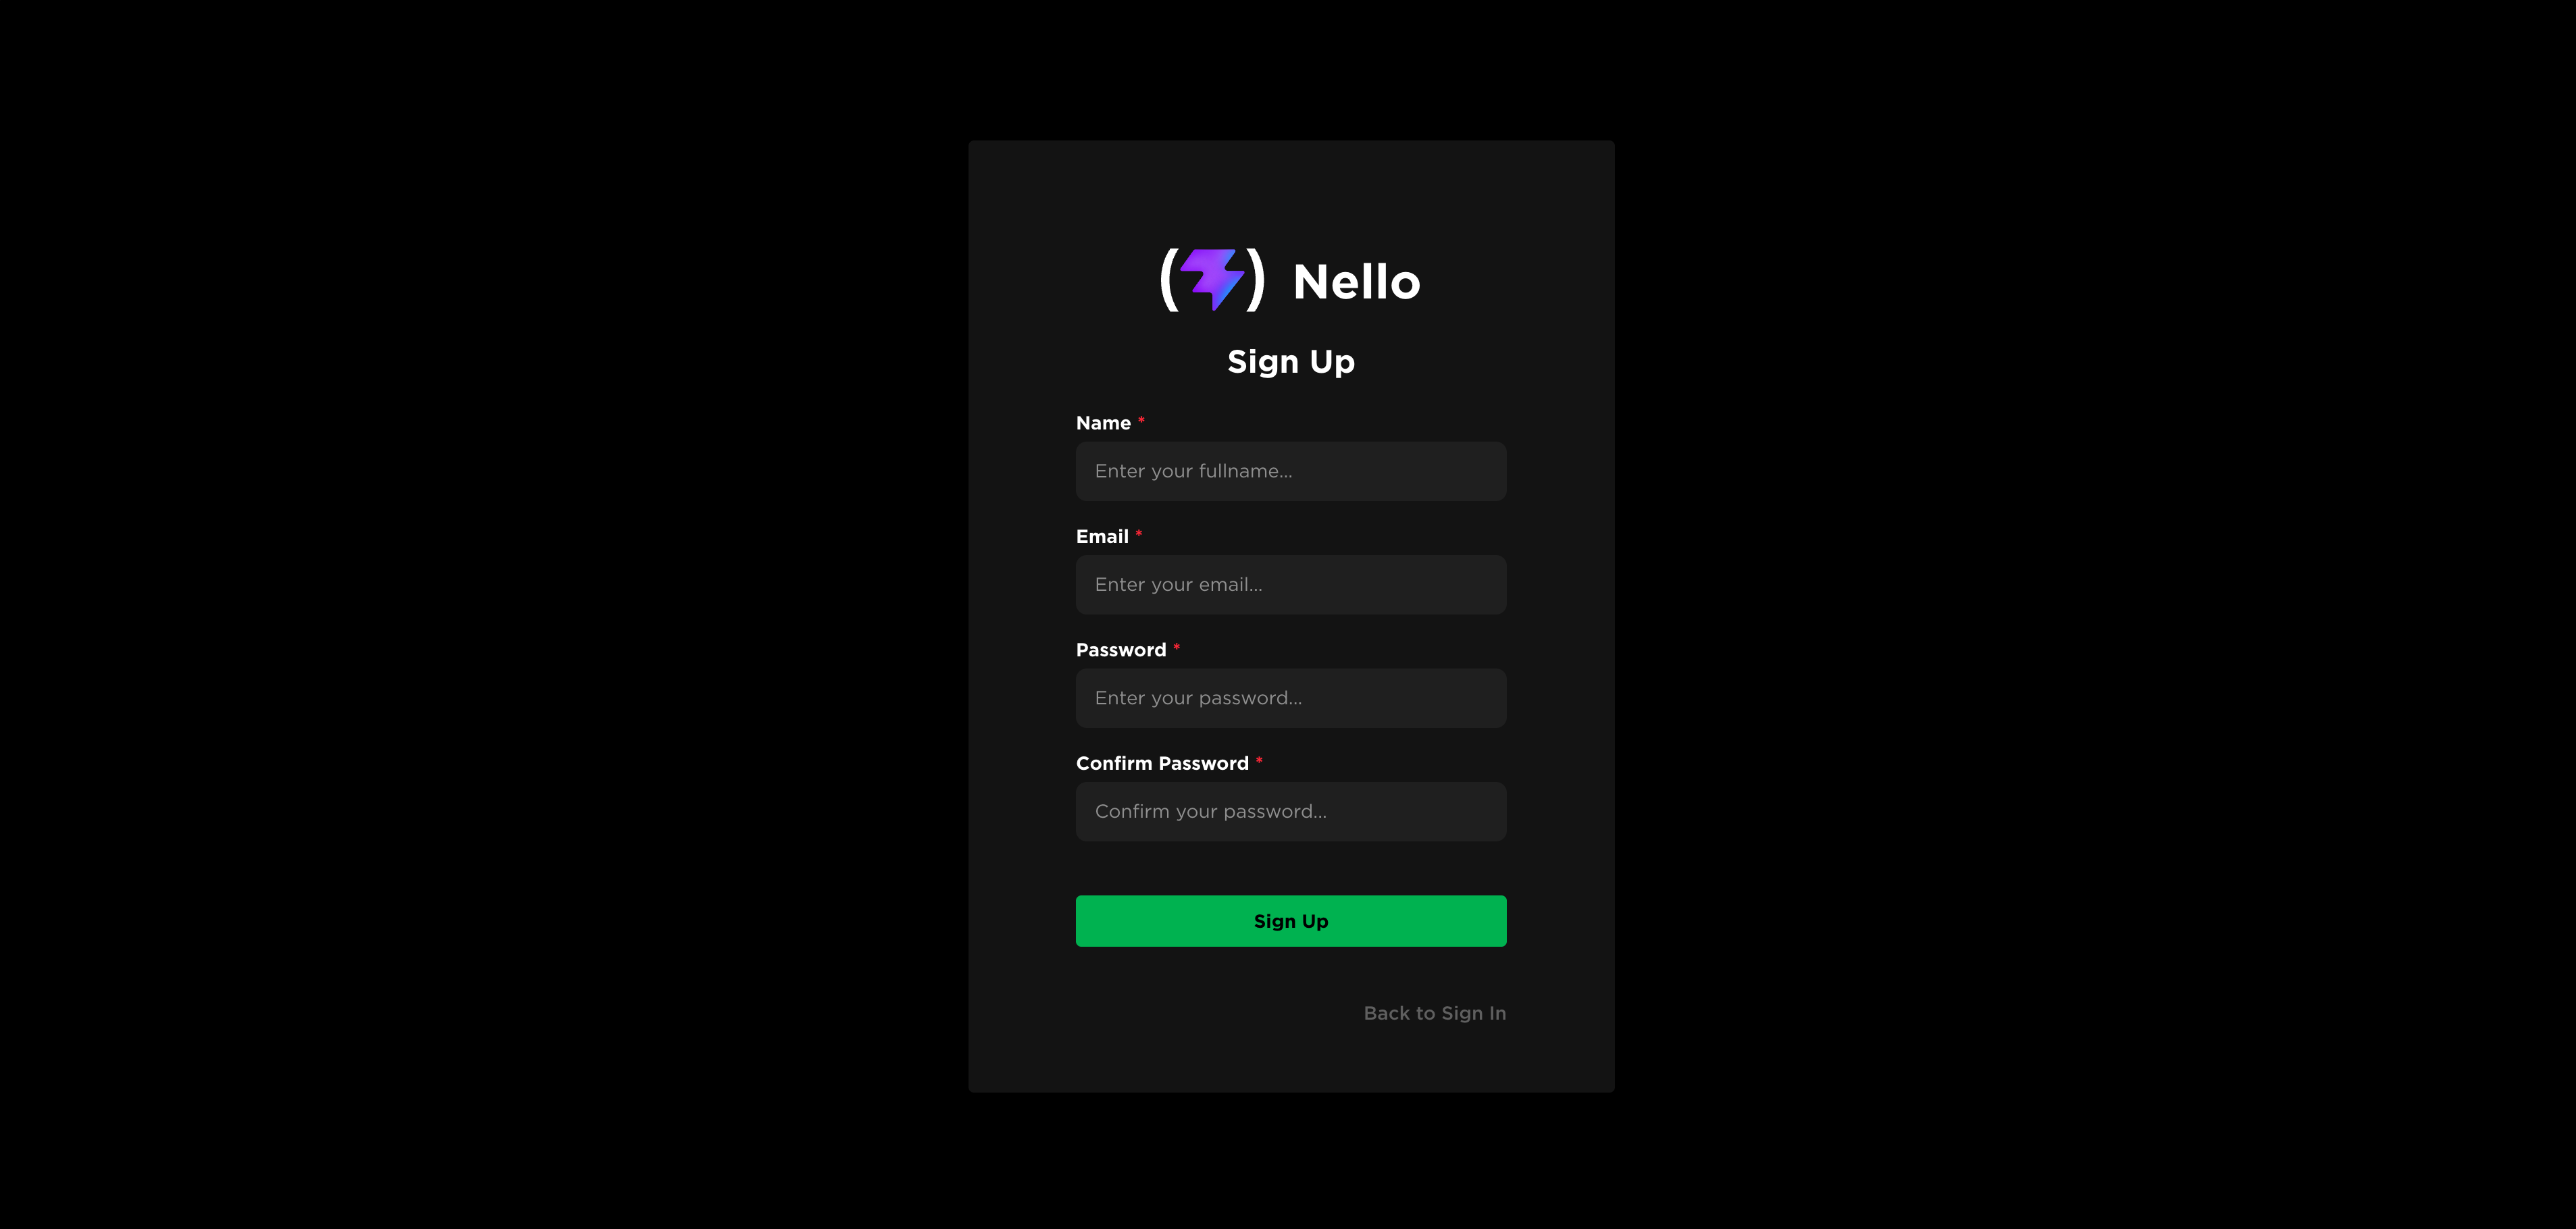
\includegraphics[width=\textwidth]{./images/chap4/screen-signup.png}
    \caption{Màn hình Đăng ký tài khoản}
    \label{fig:screen_signup}
\end{figure}

    \item \textbf{Màn hình Xác nhận OTP (\texttt{/confirm-sign-up}):} Ô nhập mã OTP 6 chữ số; nút gửi lại mã có bộ đếm thời gian; thông báo lỗi khi mã không hợp lệ; chuyển hướng về đăng nhập sau khi xác nhận.

% TODO-IMG: Chương 4 — Màn hình Xác nhận OTP (/confirm-sign-up)
\begin{figure}[H]
    \centering
    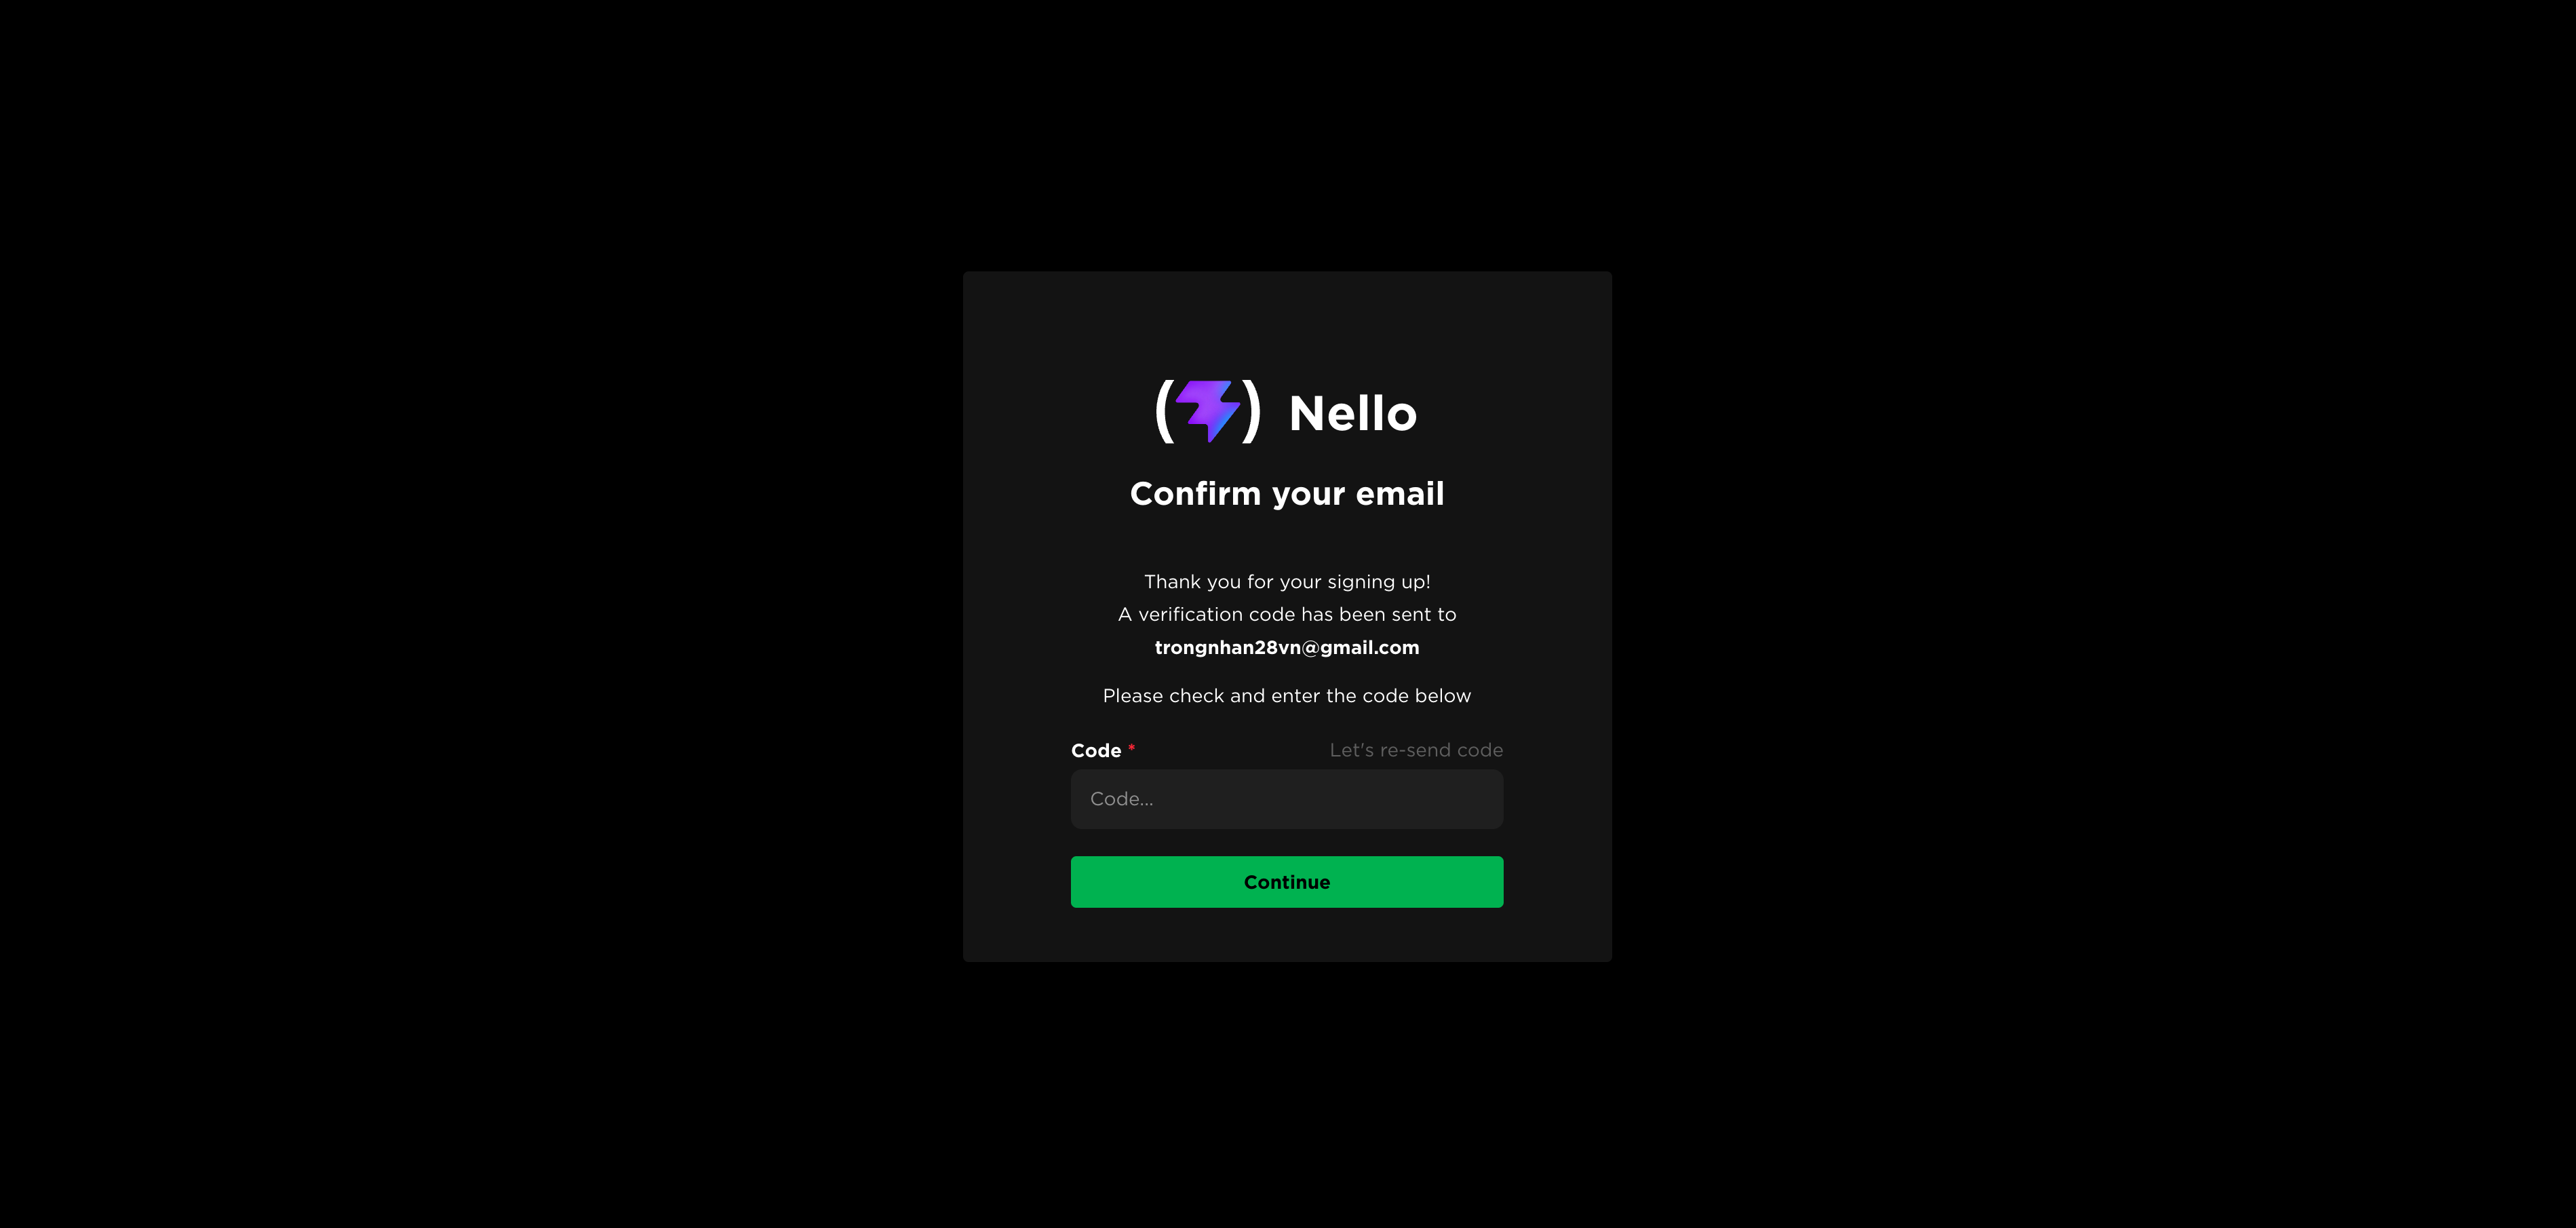
\includegraphics[width=\textwidth]{./images/chap4/screen-confirm-otp.png}
    \caption{Màn hình Xác nhận OTP}
    \label{fig:screen_confirm_otp}
\end{figure}

    \item \textbf{Màn hình Đăng nhập (\texttt{/sign-in}):} Form email và mật khẩu; thông báo lỗi khi thông tin không đúng; lưu token vào HttpOnly cookie; chuyển hướng đến Dashboard.

% TODO-IMG: Chương 4 — Màn hình Đăng nhập (/sign-in)
\begin{figure}[H]
    \centering
    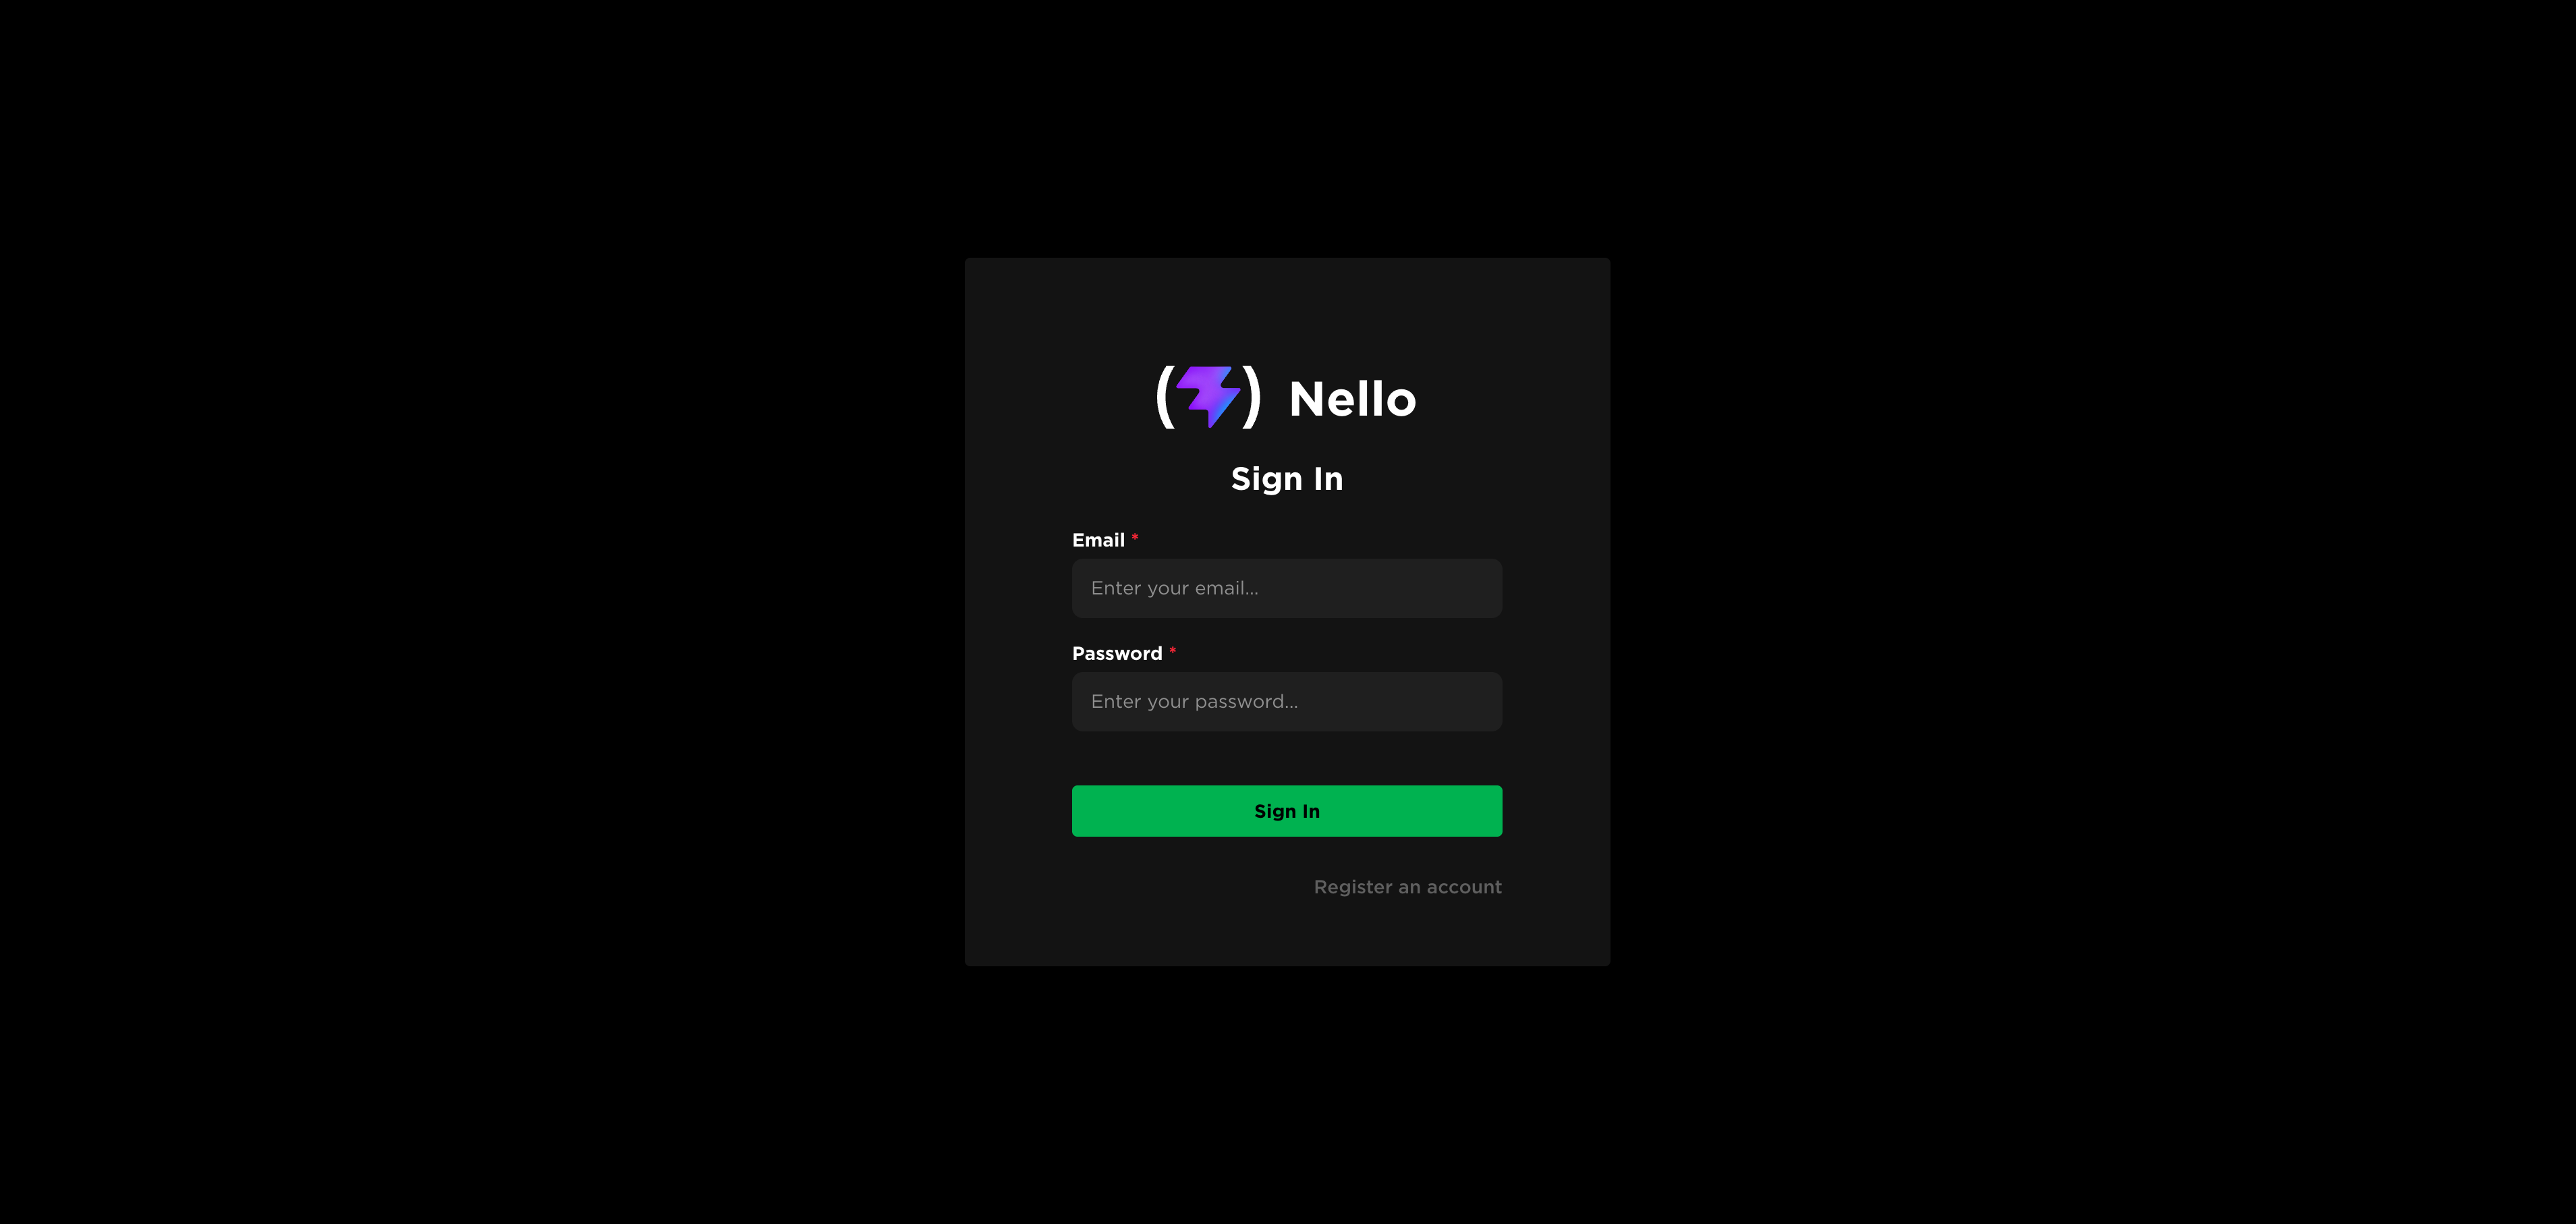
\includegraphics[width=\textwidth]{./images/chap4/screen-signin.png}
    \caption{Màn hình Đăng nhập}
    \label{fig:screen_signin}
\end{figure}

    \item \textbf{Dashboard:} Hiển thị danh sách Workspace trong sidebar; hiển thị Board theo từng Workspace dưới dạng thumbnail với ảnh nền; xử lý trạng thái trống khi chưa có dữ liệu; tự động làm mới token khi phiên hết hạn.

% TODO-IMG: Chương 4 — Màn hình Dashboard
\begin{figure}[H]
    \centering
    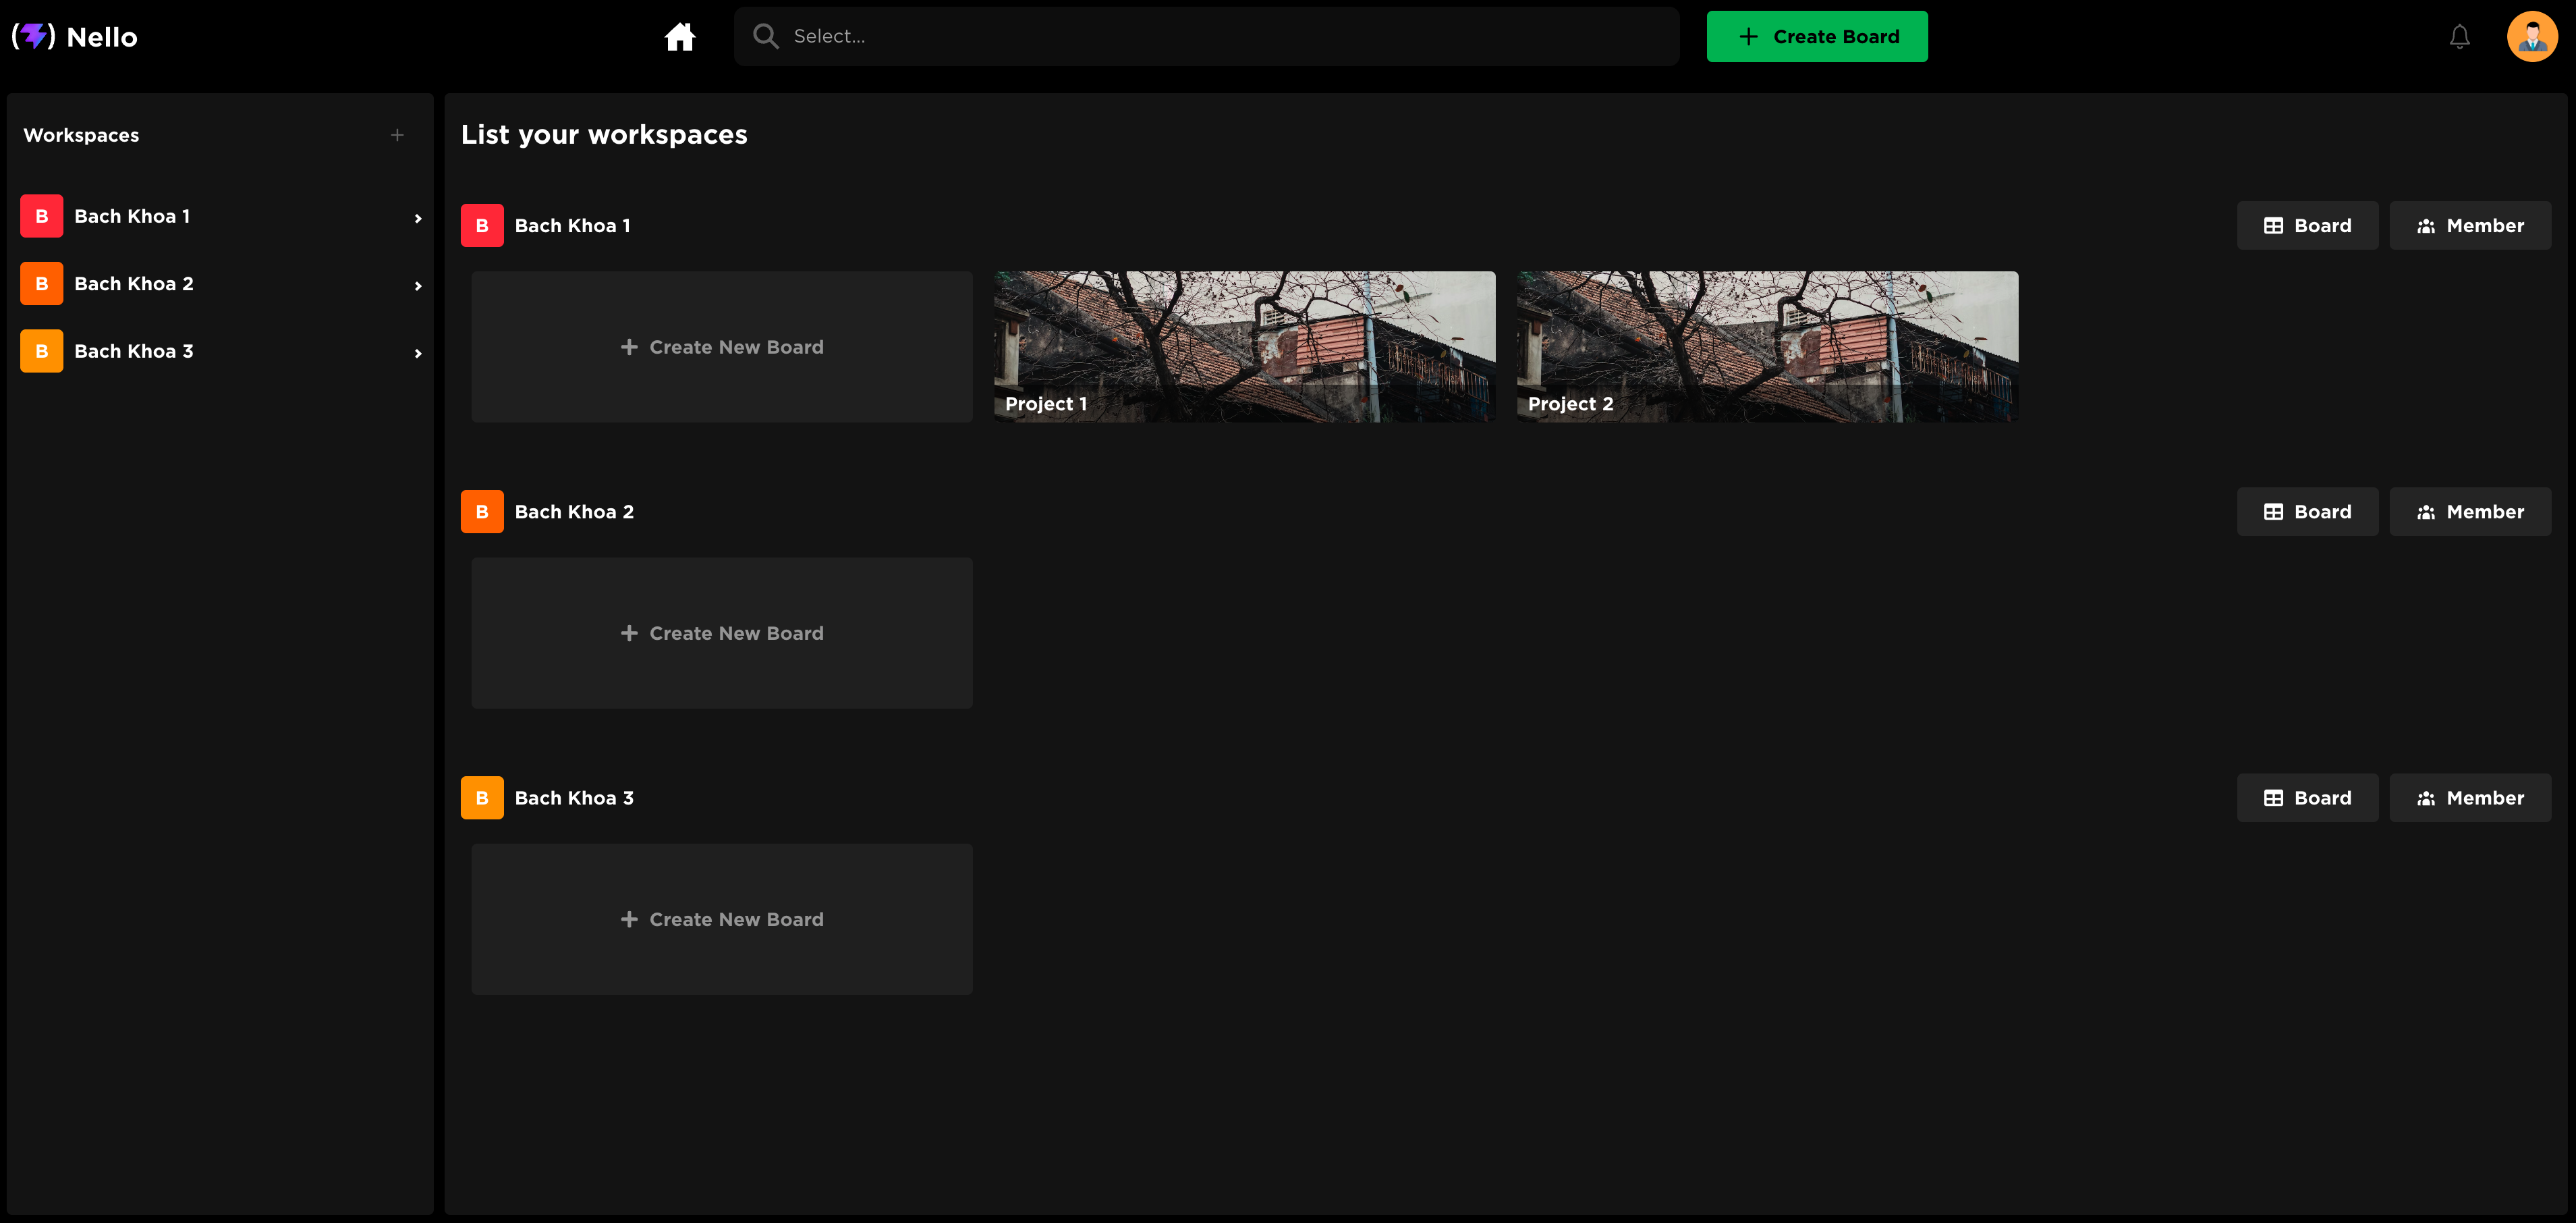
\includegraphics[width=\textwidth]{./images/chap4/screen-dashboard.png}
    \caption{Màn hình Dashboard}
    \label{fig:screen_dashboard}
\end{figure}

    \item \textbf{Màn hình Chi tiết Workspace (\texttt{/workspaces/:id}):} Thông tin Workspace, danh sách Board, danh sách thành viên với vai trò; modal mời thành viên bằng email.

% TODO-IMG: Chương 4 — Màn hình Chi tiết Workspace (/workspaces/:id)
\begin{figure}[H]
    \centering
    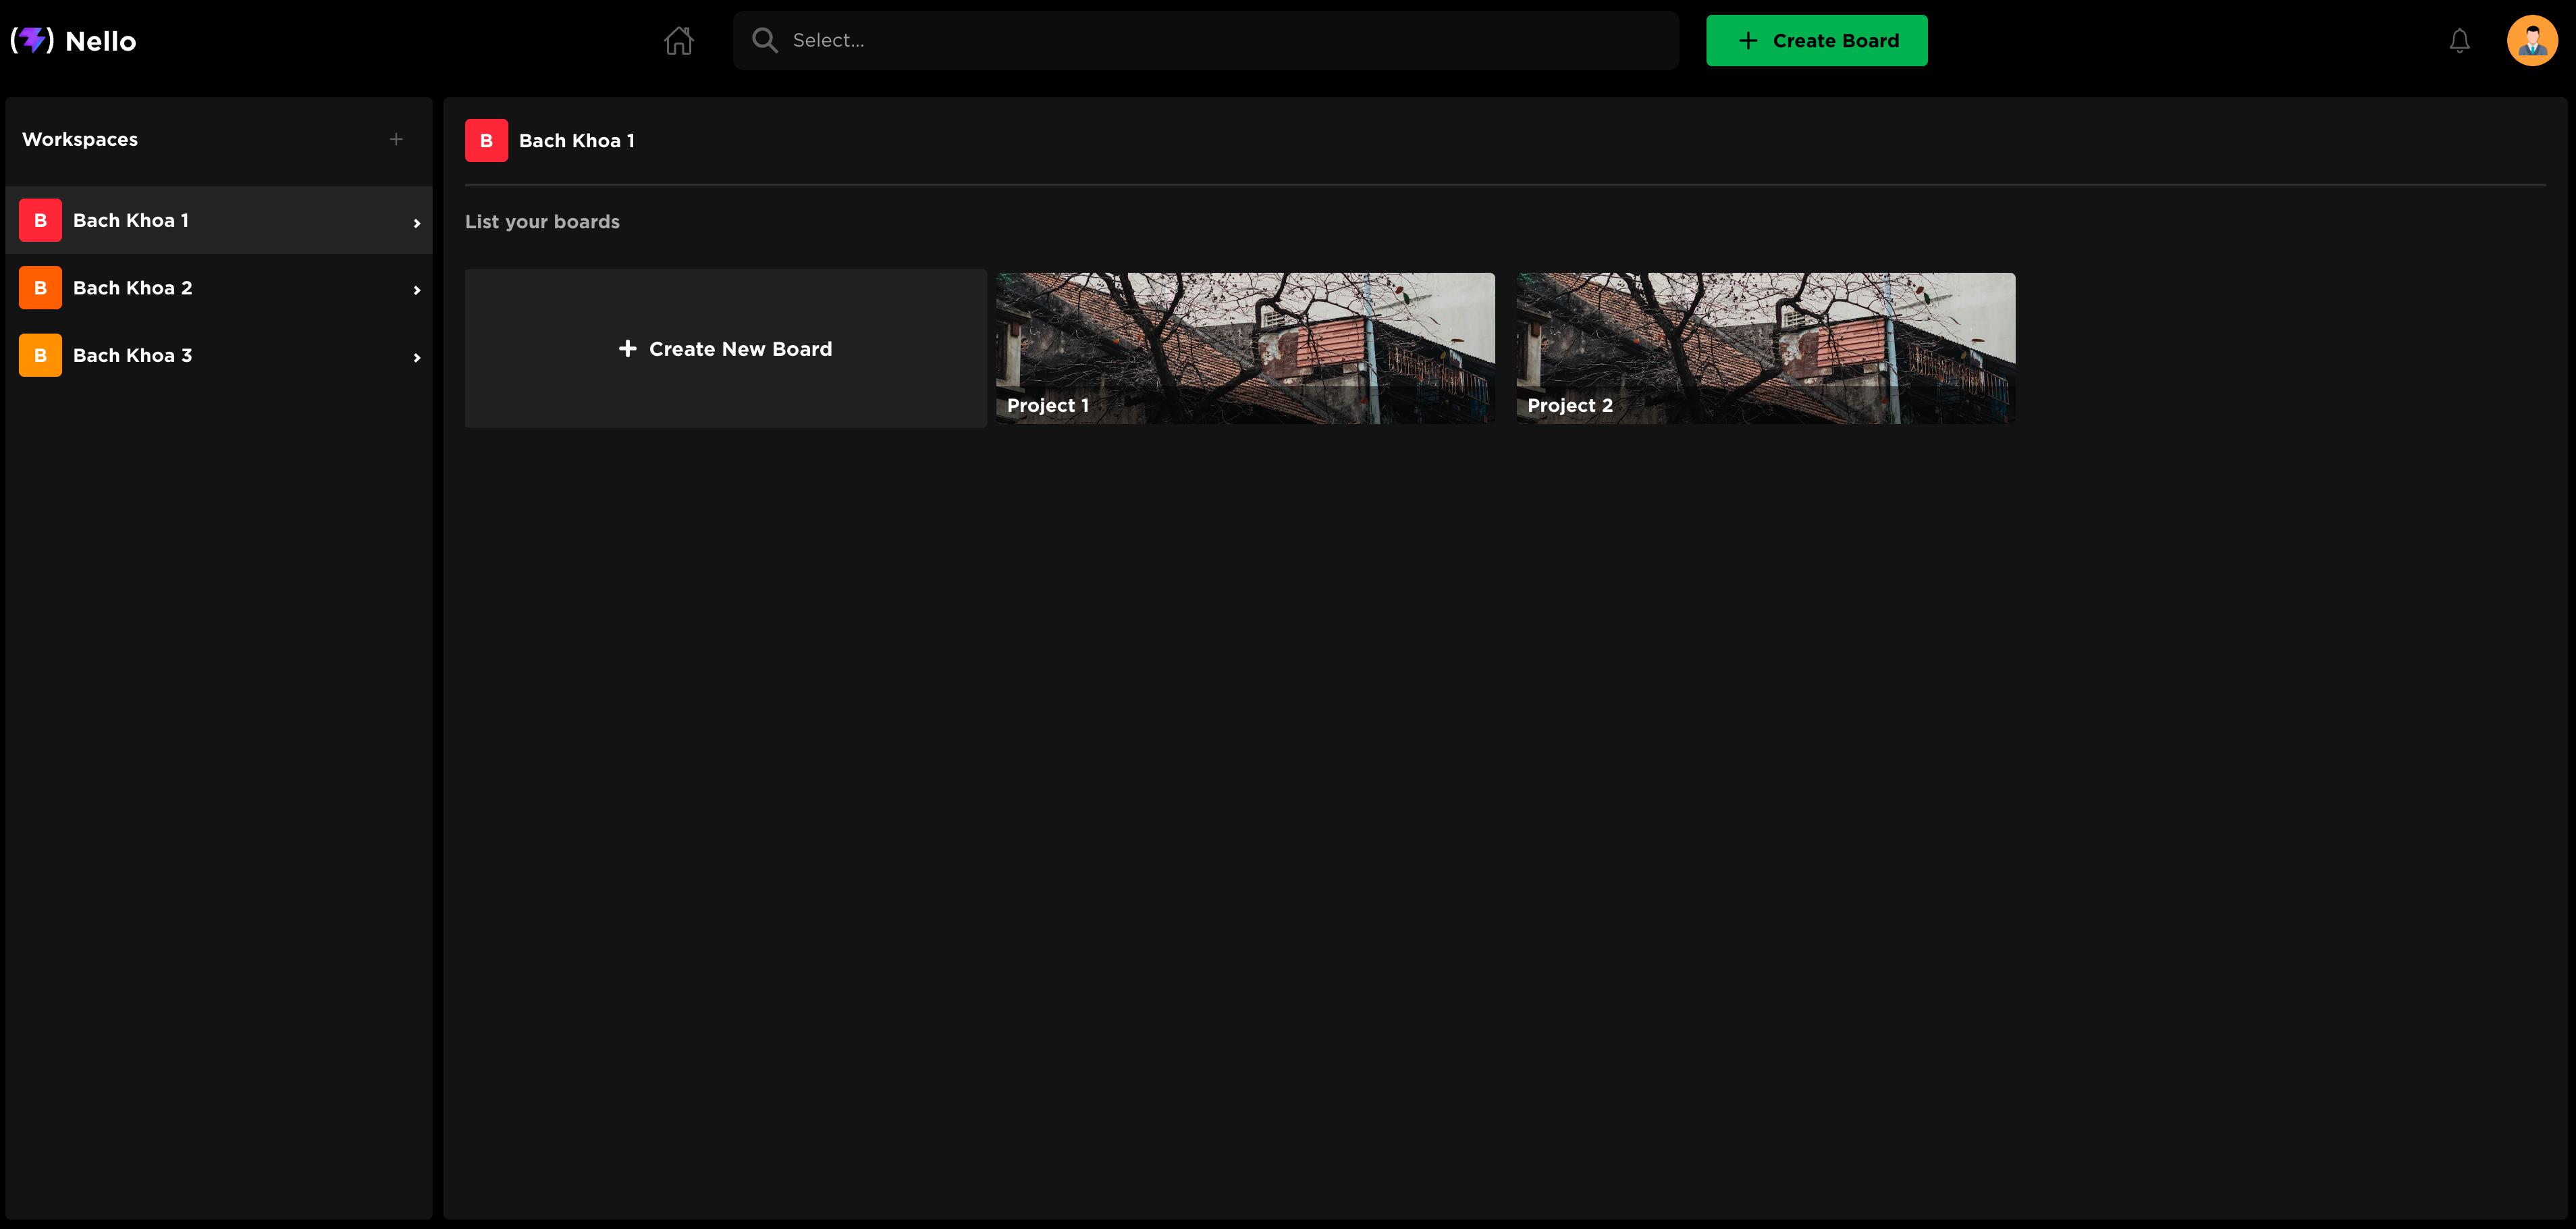
\includegraphics[width=\textwidth]{./images/chap4/screen-workspace-detail.png}
    \caption{Màn hình Chi tiết Workspace}
    \label{fig:screen_workspace_detail}
\end{figure}

    \item \textbf{Màn hình Board Kanban (\texttt{/boards/:id}):} Giao diện Kanban với các List theo dạng cột ngang; hiển thị Card trong từng List; form inline tạo List và Card; modal chi tiết Card; tính năng kéo thả List và Card; quản lý thành viên Board; badge cảnh báo Due Date; avatar thành viên trên Card.

% TODO-IMG: Chương 4 — Màn hình Board Kanban (/boards/:id)
\begin{figure}[H]
    \centering
    \includegraphics[width=\textwidth]{./images/chap4/screen-board-kanban.png}
    \caption{Màn hình Board Kanban}
    \label{fig:screen_board_kanban}
\end{figure}

\end{enumerate}

\subsection{Hình ảnh minh họa}

% TODO-IMG: Chương 4 — Minh họa tính năng kéo thả Card giữa các List
\begin{figure}[H]
    \centering
    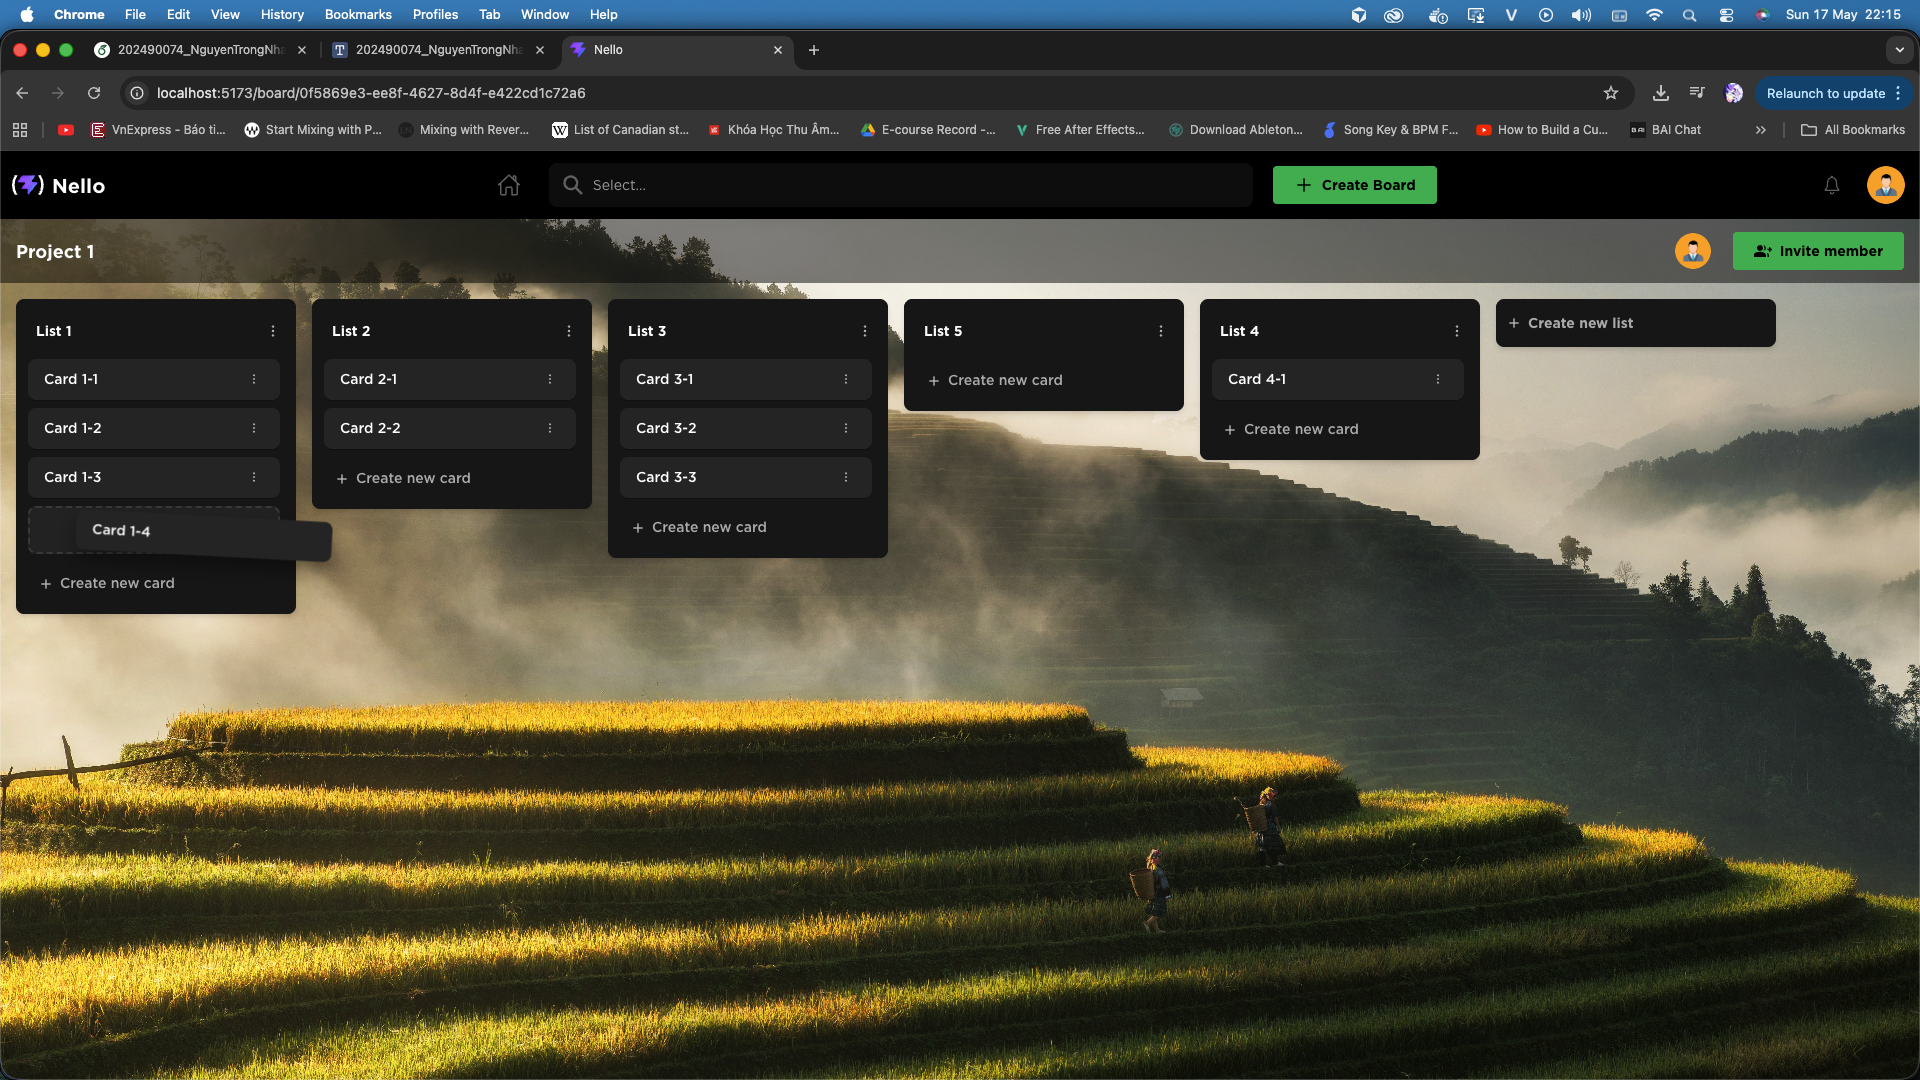
\includegraphics[width=\textwidth]{./images/chap4/feature-drag-drop.png}
    \caption{Tính năng kéo thả Card giữa các List}
    \label{fig:feature_drag_drop}
\end{figure}

% TODO-IMG: Chương 4 — Minh họa modal Chi tiết Card (Checklist, Due Date, Members)
\begin{figure}[H]
    \centering
    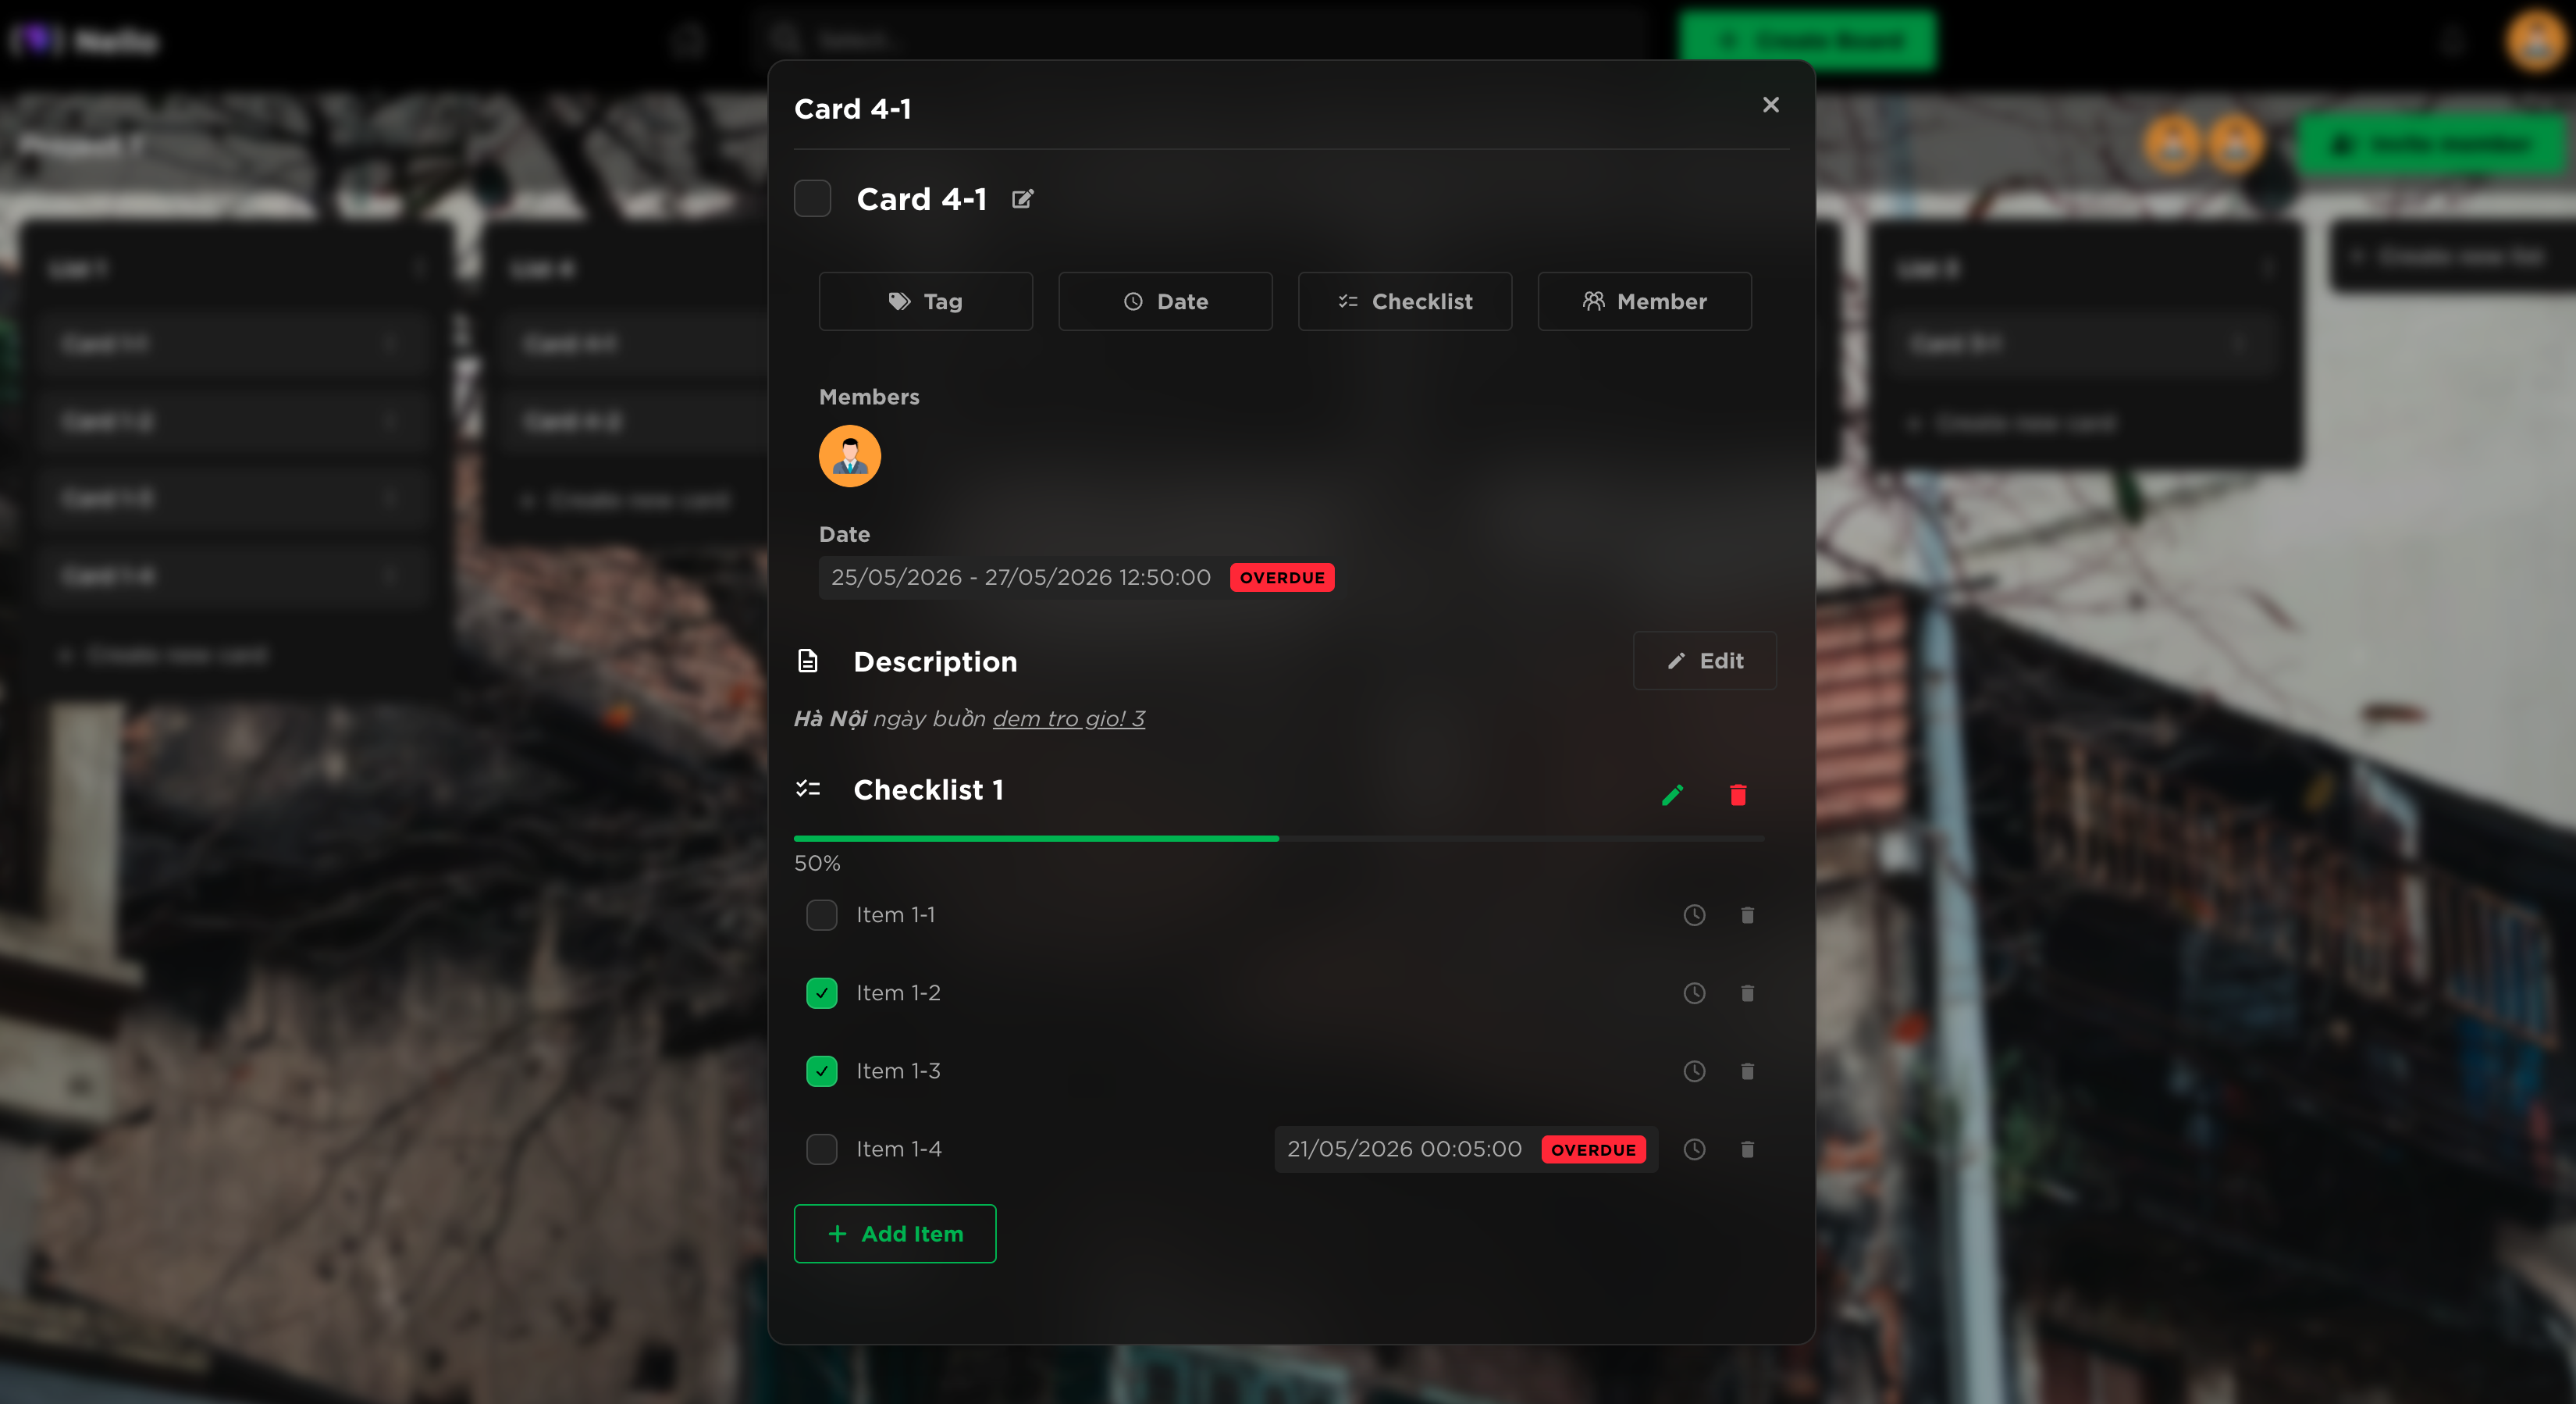
\includegraphics[width=\textwidth]{./images/chap4/feature-card-detail.png}
    \caption{Modal Chi tiết Card với Checklist, Due Date và thành viên}
    \label{fig:feature_card_detail}
\end{figure}

\subsection{Đánh giá kết quả}

\subsubsection{Ưu điểm}

Qua quá trình phát triển và kiểm thử, hệ thống quản lý công việc Nello đạt được một số ưu điểm nổi bật:

\begin{itemize}
    \item \textbf{Kiến trúc phân tách rõ ràng:} Frontend (ReactJS) và Backend (Spring Boot) hoàn toàn độc lập, tạo điều kiện bảo trì và mở rộng từng thành phần một cách linh hoạt.
    \item \textbf{Bảo mật theo tiêu chuẩn:} Toàn bộ xác thực được ủy thác cho Amazon Cognito. Token lưu trong HttpOnly cookie giúp bảo vệ khỏi tấn công XSS; tài nguyên Backend và cơ sở dữ liệu được cô lập trong mạng nội bộ VPC.
    \item \textbf{Trải nghiệm người dùng trực quan:} Giao diện Kanban quen thuộc với hỗ trợ kéo thả và cơ chế optimistic update cho phép người dùng thấy phản hồi tức thì mà không cần chờ phản hồi từ Backend.
    \item \textbf{Codebase chất lượng:} Áp dụng DTO và validation, xử lý ngoại lệ tập trung (Exception Handler), định dạng response chuẩn hóa trên toàn bộ API.
\end{itemize}

\subsubsection{Hạn chế}

Bên cạnh các kết quả đạt được, hệ thống còn tồn tại một số hạn chế cần được khắc phục trong giai đoạn tiếp theo:

\begin{itemize}
    \item \textbf{Một số chức năng chưa hoàn thiện:} Các API Backend cho phép cập nhật và xóa Workspace (FR-08, FR-30) và cập nhật Board (FR-12) đã được triển khai đầy đủ; tuy nhiên, giao diện Frontend tương ứng chưa được xây dựng. Người dùng hiện không thể thực hiện các thao tác này qua giao diện web mà chỉ có thể gọi API trực tiếp.
    \item \textbf{Kiểm thử chưa bao phủ đầy đủ các trường hợp biên và luồng lỗi:} Phần lớn các test case được thực hiện tập trung vào luồng thành công (happy case) và một số lỗi cơ bản. Các kịch bản lỗi nâng cao như dữ liệu vượt giới hạn, truy cập đồng thời, mất kết nối hoặc dữ liệu không nhất quán chưa được kiểm thử, dẫn đến nguy cơ tồn tại lỗi tiềm ẩn trong các điều kiện sử dụng thực tế.
    \item \textbf{Lỗi kéo thả ở vị trí đầu/cuối:} Thuật toán tính \texttt{position} dựa trên \texttt{beforeId}/\texttt{afterId} chưa xử lý đầy đủ các trường hợp biên khi kéo Card hoặc List về vị trí đầu tiên hoặc cuối cùng, dẫn đến sai lệch thứ tự hiển thị sau một số thao tác liên tiếp.
    \item \textbf{Phân quyền VIEWER chưa hoàn thiện:} Vai trò VIEWER được định nghĩa trong hệ thống nhưng chưa được áp dụng đầy đủ ở cả tầng Backend (kiểm tra quyền tại API endpoint) và tầng Frontend (ẩn/vô hiệu hóa các thao tác chỉnh sửa).
    \item \textbf{Chưa triển khai lên môi trường Staging:} Hệ thống hiện chỉ hoạt động trên môi trường phát triển cục bộ. Nguyên nhân chính là do xung đột cấu hình HttpOnly cookie khi Frontend và Backend được triển khai trên các domain khác nhau, đòi hỏi phải điều chỉnh chính sách \texttt{SameSite} và CORS.
    \item \textbf{Chưa có tính năng đồng bộ thời gian thực:} Hệ thống hoạt động theo mô hình request-response thuần túy. Khi một thành viên thực hiện thay đổi, các thành viên khác đang xem cùng Board cần tải lại trang thủ công để cập nhật dữ liệu, ảnh hưởng đến trải nghiệm cộng tác.
\end{itemize}

\clearpage

\section{CHƯƠNG 5: KẾT LUẬN VÀ HƯỚNG PHÁT TRIỂN}

\subsection{Kết luận}

\subsubsection{Kết quả đạt được}

Sau 8 tuần thực hiện (từ 30/03/2026 đến 24/05/2026), hệ thống quản lý công việc Nello đã được hoàn thiện với các số liệu triển khai cụ thể như sau:

\begin{table}[H]
\centering
\begin{tabular}{|p{6cm}|p{8cm}|}
\hline
\textbf{Hạng mục} & \textbf{Kết quả} \\
\hline
Thời gian thực hiện & 8 tuần (30/03/2026 – 24/05/2026) \\
\hline
Số chức năng hoàn thành & 27/31 chức năng (87,1\%) \\
\hline
Số API endpoint hoàn thành & 43 endpoint trên 14 nhóm module \\
\hline
Số màn hình Frontend & 6 màn hình chính \\
\hline
Số test case đã kiểm thử & Hơn 30 test case (tỷ lệ pass 90\%) \\
\hline
Trạng thái Backend & Hoàn chỉnh \\
\hline
Trạng thái Frontend & Hoàn chỉnh các chức năng cốt lõi \\
\hline
Môi trường triển khai & Local development \\
\hline
\end{tabular}
\caption{Tổng hợp kết quả học phần Project I}
\label{tab:final_summary}
\end{table}

Đối chiếu với các mục tiêu đề ra ban đầu, các kết quả cụ thể đạt được như sau:

\begin{itemize}
    \item \textbf{Xây dựng nền tảng quản lý khoa học:} Hoàn thành. Hệ thống hỗ trợ đầy đủ việc tổ chức công việc theo cấu trúc phân cấp Workspace $\rightarrow$ Board $\rightarrow$ List $\rightarrow$ Card, đáp ứng nhu cầu quản lý dự án đa cấp.
    \item \textbf{Quản lý thẻ công việc chi tiết:} Hoàn thành. Card hỗ trợ đầy đủ các thuộc tính gồm tiêu đề, mô tả, ngày bắt đầu, ngày đến hạn, gán thành viên và danh sách kiểm tra (Checklist) với thanh tiến độ trực quan.
    \item \textbf{Tích hợp cơ chế tương tác trực quan:} Hoàn thành. Tính năng kéo thả hoạt động ổn định cho cả List và Card trong Board, với phản hồi giao diện tức thì thông qua cơ chế optimistic update.
    \item \textbf{Đồng bộ dữ liệu và cộng tác:} Hoàn thành một phần. Các cập nhật về trạng thái công việc, phân công nhân sự và thời hạn được đồng bộ hóa với Backend sau mỗi thao tác; tuy nhiên, đồng bộ thời gian thực giữa các thành viên chưa được triển khai.
\end{itemize}

Hệ thống đã chứng minh tính khả thi của việc xây dựng một ứng dụng quản lý công việc theo mô hình Kanban với kiến trúc phân tách Frontend/Backend, tích hợp dịch vụ đám mây AWS và đảm bảo các tiêu chuẩn bảo mật cơ bản.

\subsection{Các vấn đề còn tồn tại}

\subsubsection{Chức năng chưa hoàn thiện}

Một số chức năng đã được thiết kế và triển khai ở tầng Backend nhưng giao diện Frontend tương ứng chưa được xây dựng:

\begin{itemize}
    \item Cập nhật và xóa Workspace \textbf{(FR-08, FR-30)} 
    \item Cập nhật và xóa Board \textbf{(FR-12, FR-31)}
\end{itemize}

Ngoài ra, một số tính năng đã được xác định là cần thiết nhưng nằm ngoài phạm vi thực hiện ban đầu:

\begin{table}[H]
\centering
\begin{tabular}{|p{4cm}|p{10cm}|}
\hline
\textbf{Tính năng} & \textbf{Mô tả} \\
\hline
Quản lý nhãn dán (Tag) & Tạo, gắn, tìm kiếm và lọc Card theo Tag màu sắc. \\
\hline
Hệ thống thông báo & Thông báo khi Card được giao, khi gần đến hạn hoặc khi được mời vào Workspace/Board. \\
\hline
Nhật ký hoạt động & Ghi nhận lịch sử tạo, cập nhật, xóa dữ liệu; hiển thị timeline hoạt động trong Card. \\
\hline
Board View & Xem Board theo nhiều mode view khác nhau. \\
\hline
Upload tệp đính kèm & Đính kèm tệp tin vào Card thông qua Amazon S3. \\
\hline
Đồng bộ thời gian thực & Cập nhật tự động giao diện khi thành viên khác thay đổi dữ liệu trong cùng workspace. \\
\hline
\end{tabular}
\caption{Các tính năng chưa được triển khai}
\label{tab:unimplemented_features}
\end{table}

\subsubsection{Hạn chế kỹ thuật}

\begin{itemize}
    \item \textbf{Lỗi kéo thả ở vị trí đầu/cuối danh sách:} Thuật toán tính \texttt{position} dựa trên \texttt{beforeId}/\texttt{afterId} chưa xử lý đầy đủ các trường hợp biên khi kéo Card hoặc List về vị trí đầu tiên (không tồn tại \texttt{beforeId}) hoặc vị trí cuối cùng (không tồn tại \texttt{afterId}), dẫn đến sai lệch thứ tự hiển thị sau một số thao tác kéo thả liên tiếp.
    \item \textbf{Phân quyền VIEWER chưa hoàn thiện:} Vai trò VIEWER được định nghĩa trong cơ sở dữ liệu nhưng chưa được kiểm soát đầy đủ ở tầng Backend (thiếu middleware kiểm tra quyền trên các write operation) và tầng Frontend (chưa ẩn hoặc vô hiệu hóa các nút thao tác chỉnh sửa tương ứng).
    \item \textbf{Chưa triển khai lên môi trường Staging:} Hệ thống hiện chỉ vận hành trên môi trường phát triển cục bộ. Vấn đề kỹ thuật cốt lõi là xung đột cấu hình HttpOnly cookie khi Frontend và Backend được đặt trên các domain khác nhau, đòi hỏi phải điều chỉnh chính sách \texttt{SameSite} và cấu hình CORS phù hợp với môi trường production.
    \item \textbf{Chưa có đồng bộ thời gian thực:} Hệ thống hoạt động theo mô hình request-response thuần túy. Khi một thành viên thực hiện thay đổi, các thành viên khác đang xem cùng Board cần tải lại trang thủ công để nhận cập nhật mới nhất.
    \item \textbf{Kiểm thử chưa bao phủ đầy đủ:} Phần lớn test case tập trung vào luồng thành công và một số lỗi cơ bản. Các kịch bản nâng cao như dữ liệu vượt giới hạn, truy cập đồng thời, mất kết nối mạng và dữ liệu không nhất quán chưa được kiểm thử, tiềm ẩn nguy cơ lỗi trong môi trường thực tế.
\end{itemize}

\subsection{Phương hướng phát triển}

\subsubsection{Ưu tiên cao — Hoàn thiện hệ thống hiện tại}

\begin{itemize}
    \item \textbf{Sửa lỗi thuật toán kéo thả:} Rà soát và hoàn thiện thuật toán tính \texttt{beforeId}/\texttt{afterId}, đảm bảo xử lý đúng tất cả các trường hợp biên bao gồm kéo vào đầu danh sách, cuối danh sách và danh sách trống; đồng thời đảm bảo tính nhất quán giữa trạng thái Frontend và dữ liệu Backend.
    \item \textbf{Hoàn thiện phân quyền VIEWER:} Bổ sung kiểm tra vai trò tại các API endpoint write operation ở tầng Backend và ẩn hoặc vô hiệu hóa các thành phần giao diện thao tác tương ứng khi người dùng có vai trò VIEWER.
    \item \textbf{Giải quyết vấn đề triển khai Staging:} Lựa chọn và triển khai chiến lược quản lý token phù hợp với môi trường cross-domain, bao gồm cấu hình \texttt{SameSite=None; Secure} cho cookie hoặc chuyển sang cơ chế lưu token trong \texttt{Authorization} header, sau đó tiến hành triển khai hệ thống lên môi trường Staging trên hạ tầng AWS đã thiết kế.
    \item \textbf{Hoàn thiện giao diện cập nhật và xóa Workspace/Board:} Xây dựng các màn hình và modal giao diện tương ứng cho các API FR-08, FR-12, FR-30, FR-31 đã có sẵn ở Backend.
\end{itemize}

\subsubsection{Ưu tiên trung bình — Mở rộng tính năng}

\begin{itemize}
    \item \textbf{Đồng bộ thời gian thực (Realtime Websocket):} Tích hợp Spring WebSocket với giao thức STOMP vào Backend và SockJS/STOMP client vào Frontend để đẩy sự kiện cập nhật dữ liệu (tạo, cập nhật, xóa Card; thay đổi Checklist; kéo thả) đến toàn bộ thành viên đang hoạt động trên cùng Board, nâng cao đáng kể trải nghiệm cộng tác nhóm.
    \item \textbf{Quản lý nhãn dán (Tag):} Triển khai tính năng tạo, chỉnh sửa và xóa Tag với màu sắc tùy chọn; gắn nhiều Tag cho một Card; tìm kiếm và lọc Card theo Tag trong Board.
    \item \textbf{Hệ thống thông báo (Notification):} Xây dựng cơ chế thông báo trong ứng dụng khi Card được giao cho người dùng, khi công việc sắp đến hạn hoặc đã quá hạn, và khi được mời vào Workspace hoặc Board.
\end{itemize}

\subsubsection{Ưu tiên thấp — Phát triển dài hạn}

\begin{itemize}
    \item \textbf{Nhật ký hoạt động (Activity Log):} Ghi nhận lịch sử toàn bộ thao tác tạo, cập nhật và xóa dữ liệu; hiển thị timeline hoạt động theo thời gian thực trong modal Card Detail và màn hình Board.
    \item \textbf{Các chế độ xem thay thế:} Phát triển Calendar View hiển thị Card theo due date trên lịch tháng và Timeline View trình bày tiến trình công việc theo dòng thời gian, giúp người dùng có thêm góc nhìn tổng quan về tiến độ dự án.
    \item \textbf{Upload tệp đính kèm:} Tích hợp khả năng đính kèm tệp tin vào Card thông qua Amazon S3, hỗ trợ xem trước và tải xuống trực tiếp từ giao diện Card Detail.
\end{itemize}

\clearpage